\documentclass[11pt,a4paper]{report}
%%%%%%%%%%%%%%%%%%%%%%%%%%%%%%%%%%%%%%%%%%%%%%%%%%%%%%%%%%%%%%%%%%%%%
%%                                                                 %%
%%    Header file for the Phi-S-X Series                           %%
%%                                                                 %%
%%    german version header_gm.tex is derived from header.tex      %%
%%    by uncommenting the line ``\setboolean{german}{true}'' below %%
%%                                                                 %%
%%    Never edit the german version! all changes must be done      %%
%%    in the english version header.tex                            %%
%%                                                                 %%
%%%%%%%%%%%%%%%%%%%%%%%%%%%%%%%%%%%%%%%%%%%%%%%%%%%%%%%%%%%%%%%%%%%%%
%%%%%%%%%%%%%%%%%%%%%%%%%%%%%%%%%%%%%%%%%%%%%%%%%%%%%%%%%%%%%%%%%%%%%
%%                                                                 %%
%%    Header file for the Phi-S-X Series                           %%
%%                                                                 %%
%%    german version header_gm.tex is derived from header.tex      %%
%%    by uncommenting the line ``\setboolean{german}{true}'' below %%
%%                                                                 %%
%%    Never edit the german version! all changes must be done      %%
%%    in the english version header.tex                            %%
%%                                                                 %%
%%%%%%%%%%%%%%%%%%%%%%%%%%%%%%%%%%%%%%%%%%%%%%%%%%%%%%%%%%%%%%%%%%%%%
%====================================================================
%-- define flag for language adaptations
\usepackage{ifthen}   % allows to select only certain text
\provideboolean{german}
\setboolean{german}{false}
%\setboolean{german}{true}  % uncomment this line for german editions
%====================================================================
%
% Textschriftart: Computer modern Bright
% body:            CM-Bright 10pt
% section titles:  CM-Bright Bold
% formulas:        CM-Bright Math Oblique
%
\usepackage[standard-baselineskips]{cmbright}
\usepackage{cmbright}
\usepackage[T1]{fontenc}
\def\usedfonts{CM-Bright}
\usepackage{typearea}
%\typearea[current]{calc} % benutzt die aktuelle 
       % bindekorrektur (BCOR angabe als parameter in koma usepackage)
       % und berechnet satzspiegel neu
\typearea[current]{11} %fixed div value

\usepackage{textcomp} % special symbols
\usepackage{amsfonts} % special symols
                      % see ftp://ftp.ams.org/pub/tex/doc/amsfonts/amsfndoc.pdf
\usepackage{amssymb}  % CM-Bright provides the AMS symbols
\usepackage{exscale}  % allows to scale math expressions to big fonts, 
                      % e.g. \Huge
\usepackage{curves}
\usepackage{braket}
\usepackage{miller}     % miller indices
\usepackage{chemmacros} % http://www.mychemistry.eu/mychemistry/
\usepackage[numbers]{natbib}     % bibliography style
\usepackage{url}\urlstyle{tt}
\usepackage{float}
\usepackage{bm}       % provides the command \bm{} that makes bold math symbols
\usepackage{amsmath}
\usepackage{amsbsy}   % allows bold mathematical symbols
\usepackage{amscd}
 \usepackage{a4wide}  % it is better to use the ``geometry'' package
\usepackage{array}    % 
\usepackage{fancyhdr} %  defines pagestyle fancy
\usepackage{epsfig}   % include graphics with epsfig
\usepackage{graphicx} % includegraphics
\usepackage{epstopdf}
\usepackage{wrapfig}
\usepackage{fancybox} % allows shadow-boxes
\usepackage{color}    % allows to use color in the text
%\usepackage{eepic}
\usepackage{flafter}  % places picture next to its reference
\usepackage{makeidx}  % make an index
%\usepackage{MnSymbol}  % 
%\usepackage{marvosym}  % 
\usepackage{textcase}
\usepackage{ulem} % defines strikeout \sout{}; underline \uline{}
                  % double underline \uuline{}; wave underline \uwave{}
                  % cross out \xout{}
%
%==========================================================================
%==  page layout  =========================================================
%==========================================================================
% eqnarray environment: reduce with of space in place of each ``&''
\setlength\arraycolsep{1.4pt}
\pagestyle{fancy}
%\renewcommand{\chaptermark}[1]{\markboth{\thechapter\ #1}{}}
\renewcommand{\chaptermark}[1]{\markboth{\MakeUppercase{\thechapter\ #1}}{}}
\fancyhf{} 
\fancyhead[LE]{\textsc{\thepage}\qquad\textsc{\leftmark}}
\fancyhead[RO]{\textsc{\leftmark}\qquad\textsc{\thepage}}
\renewcommand{\headrulewidth}{0.5pt}
\renewcommand{\footrulewidth}{0pt} 
\addtolength{\headheight}{2.5pt}
\fancypagestyle{plain}{\fancyhead{}
   \renewcommand{\headrulewidth}{0pt}
   \fancyfoot[CO]{\bfseries\thepage}}

% Line spacing -----------------------------------------------------------
\newlength{\defbaselineskip}
\setlength{\defbaselineskip}{\baselineskip}
\newcommand{\setlinespacing}[1]%
           {\setlength{\baselineskip}{#1 \defbaselineskip}}
\newcommand{\doublespacing}{\setlength{\baselineskip}%
                           {2.0 \defbaselineskip}}
\newcommand{\singlespacing}{\setlength{\baselineskip}{\defbaselineskip}}

% Absatz einr\"ucken ------------------------------------------------------
%\setlength{\parindent}{0pt}
\setlength{\parskip}{2pt}
% -------------------------------------------------------------------------
\ifthenelse{\boolean{german}}
  {\def\figurename{Abb.}}
  {\def\figurename{Fig.}}
%--------------------------------------------------------------------------
\renewcommand{\arraystretch}{1.15}  % skaliert den Zeilen abstand in der 
    % tabular und array umgebung
%
%==========================================================================
%==  boxes etc ============================================================
%==========================================================================
%== minipage in a shadowbox ===============================================
\newenvironment{myshadowminipage}[1]%
  {\par\noindent\begin{Sbox}\begin{minipage}{\linewidth}\vspace{0.1cm}\begin{center}\uppercase{#1}\end{center}}%
  {\vspace{0.1cm}\end{minipage}\end{Sbox}\shadowbox{\TheSbox}}
%
%== minipage in a framedbox ===============================================
\newenvironment{myframedminipage}%
  {\par\noindent\begin{Sbox}\begin{minipage}\linewidth\vspace{0.1cm}}%
  {\vspace{0.1cm}\end{minipage}\end{Sbox}\fbox{\TheSbox}}
%
\newcommand{\myshadowbox}[1]{\noindent\shadowbox{\parbox{\linewidth}{\smallskip #1\smallskip}}}
\newcommand{\myfbox}[1]{\noindent\fbox{\parbox{\linewidth}{\smallskip #1\smallskip}}\medskip}
%== minipage in a framedbox ===============================================
\newtheorem{defi}{Definition}[chapter]
\newenvironment{definition}[1]%
  {\par\noindent\begin{Sbox}\begin{minipage}{\linewidth}\vspace{0.1cm}\begin{defi}\uppercase{#1}\\\vspace{0.1cm}}%
  {\vspace{0.1cm}\end{defi}\end{minipage}\end{Sbox}\shadowbox{\TheSbox}}
%
%=========================================================================
% color used to point out information to the teacher
\definecolor{highlight}{rgb}{1.0,0.7,0.}
\newcommand{\Special}[1]{\textbf{\textcolor{highlight}{#1}}}
%=========================================================================
%  switch certain parts on and off. uses ifthen package
\newboolean{teacher}\setboolean{teacher}{false}
% this parameter can be changed in the manuscript again
\setboolean{teacher}{true} %private version if true!
\newcommand{\teacheronly}[1]{\ifthenelse{\boolean{teacher}}{#1\hfill\\ }}
\newcommand{\editor}[1]{\textcolor{blue}{\texttt{Editor: #1}}}
\newcommand{\MARK}[1]{\textcolor{blue}{#1}} 
\newcommand{\RED}[1]{\textcolor{red}{#1}} 
%
%==========================================================================
%==  define new symbols                                                 ===
%==========================================================================
% define \stat (stationary state) as an operator like \min
\DeclareMathOperator*{\stat}{stat}
\let\Vec=\mathbold   % cmbright.sty provides a bold/italic math alphabet
\let\Dot=\mathbold   % cmbright.sty provides a bold/italic math alphabet
\let\Ddot=\mathbold   % cmbright.sty provides a bold/italic math alphabet
%
\newcommand{\e}[1]{\mathrm{e}^{#1}}% exponential function
\renewcommand{\Re}{\mathrm{Re}}    % real part
\renewcommand{\Im}{\mathrm{Im}}    % imaginary part
\newcommand{\lagr}{\ell}           % Lagrange dichte
\newcommand{\Lagr}{\mathcal{L}}    % Lagrange Funktion
\newcommand{\erf}{{\rm erf}}       %
\newcommand{\atan}{{\rm atan}}     % arcus tangens
\newcommand{\mat}[1]{\bm{#1}}  % Matrix
\newcommand{\gmat}[1]{{\boldsymbol #1}}  % Matrix(symbol)
\newcommand{\defas}{\stackrel{\text{def}}{=}}  %  is defined as
\ifthenelse{\boolean{german}}
  {\newcommand{\rot}{{\rm\bf rot}}}    % curl
  {\newcommand{\rot}{{\rm\bf curl}}}   % curl
\newcommand{\sgn}{{\rm sgn}}       % sign
\ifthenelse{\boolean{german}}
   {\newcommand{\Tr}{\mathrm{Sp}}}      % trace
   {\newcommand{\Tr}{\mathrm{Tr}}}      % trace
\ifthenelse{\boolean{german}}
   {\newcommand{\grmn}[2]{\footnote{``#2'' hei{\ss}t in englisch ``#1''}}}
   {\newcommand{\grmn}[2]{\footnote{``#1'' translates as ``#2'' into German}}}
% define the equation reference
\ifthenelse{\boolean{german}}
   {\newcommand{\eq}[1]{\text{Gl.}~\ref{#1}}}
   {\newcommand{\eq}[1]{\text{Eq.}~\ref{#1}}}
% define a relation with an equation number ontop
\newcommand{\eqrel}[2]{\stackrel{\eq{#1}}{#2}}
\newcommand{\zero}{\varnothing}
%\newcommand{\ket}[1]{|#1\rangle} % contained in package braket
\newcommand{\sumint}{\int\hspace{-15pt}\sum}
\newcommand{\marker}[1]{\textcolor{blue}{\emph{#1}}}
\renewcommand*{\dot}[1]{\overset{\mbox{\large\bfseries .}}{#1}}
\renewcommand*{\ddot}[1]{\overset{\mbox{\large\bfseries\hspace{+0.1ex}.\hspace{-0.1ex}.}}{#1}}
%
%==========================================================================
%==                                                                     ===
%==========================================================================
% Prevent figures from appearing on a page by themselves
% from http://dcwww.camd.dtu.dk/~schiotz/comp/LatexTips/LatexTips.html
\renewcommand{\topfraction}{0.85}
\renewcommand{\textfraction}{0.1}
\renewcommand{\floatpagefraction}{0.75}
%
%==========================================================================
%==                                                                     ===
%==========================================================================
\makeindex    % make index. uses makeidx package.

%== allow links between documents ============================================
\usepackage{xr}
\usepackage{xr-hyper}
%==  hyperref package (must be last package)
\usepackage[colorlinks=true]{hyperref} %specify this as last package
\hypersetup{citecolor=blue}
\hypersetup{menucolor=magenta}
\hypersetup{urlcolor=blue}      % 
\hypersetup{filecolor=green}    % file links
\hypersetup{linkcolor=magenta}  %table of contents
\hypersetup{pdfauthor={Peter E. Bl\"ochl}}
\hypersetup{pdfdisplaydoctitle=true}
\externaldocument[phisx1-]{/Users/ptpb/Tree/PhiSX/ClassicalMechanics/Book/cm-gm}
\externaldocument[phisx2-]{/Users/ptpb/Tree/PhiSX/Electrodynamics/Book/el-gm}
\externaldocument[phisx3-]{/Users/ptpb/Tree/PhiSX/QuantumMechanics/Book/qm}
\externaldocument[phisx4-]{/Users/ptpb/Tree/PhiSX/StatisticalMechanics/Book/sm}
\externaldocument[phisxqm2-]{/Users/ptpb/Tree/PhiSX/QuantumMechanicsII/Book/qm2}
\externaldocument[phisxsm2-]{/Users/ptpb/Tree/PhiSX/StatisticalMechanicsII/Book/sm2}
\externaldocument[phisxcb-]{/Users/ptpb/Tree/PhiSX/Chemicalbond/Book/cb}
% Example: Figure~PhiSX:Quantum
% Mechanics-\ref{phisx3-fig:doubleslitwave} on page
% \pageref{phisx3-fig:doubleslitwave}


\hypersetup{pdftitle=paw_brillouin}
\newcommand{\petertt}[1]{\textcolor{red}{\texttt{#1}}}
\begin{document}
\begin{titlepage}
\begin{center}
\vspace*{3.5cm}
{\huge \textbf{The DMFT object of the CP-PAW code}}\\
\vspace{0.5cm}
{\large Peter E. Bl\"ochl}
\vspace{0.5cm} 
\end{center}

\vfill
\begin{center}
Copyright Peter E. Bl\"ochl; Sept.2, 2013-\today\\
{\small
Institute of Theoretical Physics;
Clausthal University of Technology;\\ 
D-38678 Clausthal Zellerfeld; Germany;\\
http://www.pt.tu-clausthal.de/atp/}
\end{center}
\end{titlepage}
\noindent            
\tableofcontents
%====================================================================
\chapter{Purpose and theoretical background}
%====================================================================
The purpose of the DMFT object is to prepare an interface to the
solver for a quantum impurity in the context of dynamical mean-field
theory. The derivations follow closely the paper of Bl\"ochl,
Pruschke and Potthoff\cite{bloechl13_prb88_25139}, in the following
referred to \textbf{BPP}\index{BPP}.

%====================================================================
\section{Grand potential and density-matrix 
functional as starting point}
%====================================================================
The \textbf{grand potential}\index{grand potential}
 has the form\cite{bloechl13_prb88_25139}
\begin{eqnarray}
\Omega^{KB}_{\beta,\mu}[\hat{h}+\hat{W}]
&=&\min_{|\psi_n\rangle,f_n\in[0,1]}\stat_\Lambda
\biggl\lbrace\sum_n f_n\langle\psi_n|\hat{h}|\psi_n\rangle
+\tilde{F}_\beta^{\hat{W}}\Bigl[\sum_n|\psi_n\rangle f_n\langle\psi_n|\Bigr]
-\mu\sum_n f_n\nonumber\\
&&
-\sum_{m,n}\Lambda_{m,n}\Bigl(\langle\psi_n|\psi_m\rangle-\delta_{m,n}\Bigr)
\biggr\rbrace
\label{eq:gcpdm2}
\end{eqnarray}
where the \textbf{density-matrix functional}\index{density-matrix
  functional} $\tilde{F}_\beta^{\hat{W}}$ is
expressed\cite{bloechl13_prb88_25139} by the \textbf{Luttinger-Ward
  functional}\index{Luttinger-Ward functional}
\cite{luttinger60_pr118_1417} $\Phi^{LW}[\mat{G},\hat{W}]$ as
\begin{eqnarray}
\tilde{F}^{\hat{W}}_\beta[\mat{\rho}]
&=&
\frac{1}{\beta}\Tr\Bigl[
\mat{\rho}\ln(\mat{\rho})+(\mat{1}-\mat{\rho})\ln(\mat{1}-\mat{\rho})\Bigr]
\nonumber\\
&+&
\stat_{\mat{h}'}\stat_{\mat{G},\mat{\Sigma}}
\biggl\lbrace
\Phi^{LW}_\beta[\mat{G},\hat{W}]
-\frac{1}{\beta}\sum_\nu\Tr\Bigl\lbrace
\ln\Bigl[
\mat{1}-
\Bigl(i\hbar\omega_\nu+\mu)\mat{1}-\bar{\mat{h}}\Bigr)^{-1}
\Bigl(\mat{h}'+\mat{\Sigma}(i\omega_\nu)-\bar{\mat{h}}\Bigr)
\Bigr]
\nonumber\\&&
+(\mat{h}'+\mat{\Sigma}(i\omega_\nu)-\bar{\mat{h}})\mat{G}(i\omega_\nu)
-
\Bigl[
\mat{G}(i\omega_\nu)
-\Bigl(i\hbar\omega_\nu+\mu)\mat{1}-\bar{\mat{h}}\Bigr)^{-1}
\Bigr]
\Bigl(\mat{h}'-\bar{\mat{h}}\Bigr)\Bigr\rbrace
\biggr\rbrace
\label{eq:dmfgreen}
\end{eqnarray}
Here, $|\psi_n\rangle$ are one-particle wave functions. They play the
role of \textbf{natural orbitals}\index{natural orbitals}, the
eigenstates of the \textbf{one-particle density
  matrix}\index{one-particle density matrix}\index{density matrix}
$\mat{\rho}$. $f_n$ are the \textbf{occupations}\index{occupation},
the eigenvalues of the one-particle density matrix. The orthonormality
of the natural orbitals is enforced with the method of Lagrange
multipliers. The Lagrange multipliers are $\Lambda$. The chemical
potential is $\mu$ and $\beta=1/(k_BT)$. The full Hamiltonian consists
of a non-interacting part
$\hat{h}=\frac{\hat{p}^2}{2m_0}+\hat{v}_{ext}$ and an
electron-electron interaction $\hat{W}$.

With $\stat_x Y$, we denote the \textbf{stationary
  condition}\index{stationary condition}, which requires that the
partial derivative of $Y$ with respect to the variable $x$
vanishes. It explicitely does not require the stationary point to be
an extremum.

$\mat{G}(i\omega)$ is the Green's function and
$\mat{\Sigma}(i\omega_\nu)$ is the self energy.  The Matsubara sum
runs over the \textbf{Matsubara frequencies}\index{Matsubara
  frequencies} (see appendix~\ref{app:matsubarafreq} on
p.~\pageref{app:matsubarafreq})
\begin{eqnarray}
\omega_\nu=(2\nu-1)\frac{\pi}{\hbar\beta}
\qquad\text{for $\nu\in\mathbb{Z}$}
\end{eqnarray}

$\mat{h}'$ are the Lagrange multipliers for the \textbf{density-matrix
  constraint}\index{density-matrix constraint}.
\begin{eqnarray}
\mat{\rho}=\frac{1}{\beta}
\sum_\nu\e{i\beta\hbar\omega_\nu0^+}\mat{G}(i\omega_\nu)
\label{eq:rhoofg}
\end{eqnarray}

The Hamiltonian $\bar{\mat{h}}$ is a non-local Hamiltonian directly
related to the one-particle density matrix via (see Eq.~BPP24)
\begin{eqnarray}
\bar{\mat{h}}=\mu\mat{1}+k_BT\ln
\left[\frac{\mat{1}-\mat{\rho}}{\mat{\rho}}\right]
\label{eq:defhbar}
\end{eqnarray}



In practice, we perform calculations at fixed particle
number. Therefore, we calculate the \textbf{Helmholtz
  potential}\index{Helmholtz potential} by adding the term with the
particle number $N$ to the grand potential.
\begin{eqnarray}
A_{\beta,N}[\hat{h}+\hat{W}]
&=&\stat_\mu\Bigl\lbrace\Omega_{\beta,\mu}+\mu N\Bigr\rbrace
\nonumber\\
&=&\min_{|\psi_n\rangle,f_n\in[0,1]}\stat_{\mu,\Lambda}
\biggl\lbrace\sum_n f_n\langle\psi_n|\hat{h}|\psi_n\rangle
+Q_\beta^{\hat{W}}\Bigl[\sum_n|\psi_n\rangle f_n\langle\psi_n|\Bigr]
\nonumber\\
&&+\frac{1}{\beta}\sum_n\Bigl[f_n\ln(f_n)+(1-f_n)\ln(1-f_n)\Bigr]
\nonumber\\
&&
-\mu\Bigl[\sum_n f_n-N\Bigr]
-\sum_{m,n}\Lambda_{m,n}\Bigl(\langle\psi_n|\psi_m\rangle-\delta_{m,n}\Bigr)
\biggr\rbrace
\label{eq:hp}
\end{eqnarray}
where $Q^{\hat{W}}_\beta$ is the density-matrix functional without the
entropy contribution of a non-interacting electron gas with the same
density matrix.  The entropy contribution is taken care of with the
\textbf{Mermin functional}\index{Mermin
  functional}\cite{mermin65_pr137_a1441} to describe DFT calculations
with electrons at finite temperature.
\begin{eqnarray}
Q^{\hat{W}}_\beta[\mat{\rho}]
&=&\tilde{F}^{\hat{W}}_\beta[\mat{\rho}]
-
\frac{1}{\beta}\Tr\Bigl[
\mat{\rho}\ln(\mat{\rho})+(\mat{1}-\mat{\rho})\ln(\mat{1}-\mat{\rho})\Bigr]
\nonumber\\
&=&
\stat_{\mat{h}'}\stat_{\mat{G},\mat{\Sigma}}
\biggl\lbrace
\Phi^{LW}_\beta[\mat{G},\hat{W}]
-\frac{1}{\beta}\sum_\nu\Tr\Bigl\lbrace
\ln\Bigl[
\mat{1}-
\Bigl(i\hbar\omega_\nu+\mu)\mat{1}-\bar{\mat{h}}\Bigr)^{-1}
\Bigl(\mat{h}'+\mat{\Sigma}(i\omega_\nu)-\bar{\mat{h}}\Bigr)
\Bigr]
\nonumber\\&&
+(\mat{h}'+\mat{\Sigma}(i\omega_\nu)-\bar{\mat{h}})\mat{G}(i\omega_\nu)
-
\Bigl[
\mat{G}(i\omega_\nu)
-\Bigl(i\hbar\omega_\nu+\mu)\mat{1}-\bar{\mat{h}}\Bigr)^{-1}
\Bigr]
\Bigl(\mat{h}'-\bar{\mat{h}}\Bigr)\Bigr\rbrace
\biggr\rbrace
\label{eq:dmfQgreen}
\end{eqnarray}

%====================================================================
\section{Separate out static correlations: Towards DFT+}
%====================================================================
In appendix~\ref{sec:sdlitcorrelation} it is shown that the
correlation contribution $Q^{\hat{W}}_\beta$ can be divided into one
part having a frequency-dependent \textbf{self
  energy}\index{self-energy} and several contributions having a
frequency-independent self energy. When we talk about a self energy in
the context of the density-matrix functional theory, we refer to the
construction of the density matrix functional from an optimization of
Green's functions.\cite{bloechl13_prb88_25139} The Luttinger-Ward
functional with frequency-independent self energy can be expressed by
the density matrix alone, that is, the Green's function enters always
in the form of the integral
\begin{eqnarray}
\frac{1}{\beta}\sum_\nu\mat{G}(i\omega_\nu)\e{i\hbar\omega\beta0^+}
\end{eqnarray}

According to appendix~\ref{sec:sdlitcorrelation} on
p.~~\pageref{sec:sdlitcorrelation}, this notion allows us to split the
interaction contribution $Q^{\hat{W}}$ into different parts as
\begin{eqnarray}
Q^{\hat{W}}[\mat{\rho}]
\approx Q^{DFT,\hat{W}}[\mat{\rho}]-Q^{DFT,\hat{W}_1}[\mat{\rho}]
+Q^{HF,\hat{W}_1}[\mat{\rho}]-Q^{HF,\hat{W}_2}[\mat{\rho}]
+Q^{\hat{W}_2}[\mat{\rho}]
\label{eq:splitq}
\end{eqnarray}
of which only the last term has a frequency-dependent self energy.

In order to keep the computational effort at a reasonable level, we
consider three different interactions, namely the full interaction
$\hat{W}$, a simplified interaction $\hat{W}_1$ used for static
correlations, and interaction $\hat{W}_2$, which is even further
simplified, and which is used for dynamic correlations.
The full interaction is treated on the most simple level of the
description, namely DFT, while the most complex many-particle
treatment is limited to the most approximate interaction, namely
$\hat{W}_2$. 

With a density-functional contribution $Q^{DFT,\hat{W}}[\hat{\rho}]$
acting as double-counting term and a screened Hartree-Fock
contribution $Q^{HF,\hat{W}}[\hat{\rho}]$ described later, we obtain
\begin{myshadowminipage}{Helmholtz potential}
\begin{eqnarray}
A_{\beta,N}[\hat{h}+\hat{W}]
&=&\min_{|\psi_n\rangle,f_n\in[0,1]}\stat_{\mu,\Lambda}
\biggl\lbrace
\sum_n f_n\langle\psi_n|\frac{\hat{\vec{p}}^2}{2m_e}|\psi_n\rangle
+\int d^3r\;n(\vec{r})v_{ext}(\vec{r'})
\nonumber\\
&&+\frac{1}{2}\int d^3r\int d^3r'
\frac{e^2n(\vec{r})n(\vec{r'})}{4\pi\epsilon_0|\vec{r}-\vec{r'}|}
+E_{xc}[n]
+\frac{1}{\beta}\sum_n\Bigl[f_n\ln(f_n)+(1-f_n)\ln(1-f_n)\Bigr]
\nonumber\\
&&+
\underbrace{Q_{\beta}^{HF,\hat{W}_1}[\mat{\rho}]
   -Q_{\beta}^{DFT,\hat{W}_1}[\mat{\rho},n]}_{\text{local hybrid functional}}
\quad+\quad
\underbrace{Q_{\beta}^{\hat{W}_2}[\mat{\rho}]
-Q_{\beta}^{HF,\hat{W}_2}[\mat{\rho}]}
_{Q_{\beta}^{dyn,\hat{W}_2}[\mat{\rho}]}
\nonumber\\
&&
-\mu\Bigl[\sum_n f_n-N\Bigr]
-\sum_{m,n}\Lambda_{m,n}\Bigl(\langle\psi_n|\psi_m\rangle-\delta_{m,n}\Bigr)
\biggr\rbrace
\label{eq:hp}
\end{eqnarray}
where 
\begin{eqnarray}
n(\vec{r},\sigma,\sigma')&=&
\sum_n\langle\vec{r},\sigma|\psi_n\rangle 
f_n\langle\psi|\vec{r},\sigma'\rangle 
\nonumber\\
n(\vec{r})&=&\sum_\sigma n(\vec{r},\sigma,\sigma)
\nonumber\\
\rho_{a,b}&=&\sum_n\langle\pi_a|\psi_n\rangle 
f_n\langle\psi|\pi_b\rangle 
\label{eq:denmatmatel}
\end{eqnarray}
\end{myshadowminipage}

We distinguish two different corrections:
\begin{enumerate}
\item a screened Hartree-Fock correction with an interaction
  $\hat{W}_1$. 

  The Hartree-Fock term $Q^{HF,\hat{W}}_{\beta}$ is equal to
  $Q^{\hat{W}}_\beta$ when only the first-order term of the
  Luttinger-Ward functional in the interaction is considered.  It is
  obtained as (BPP-Eq.43)
  \begin{eqnarray}
  Q_{\beta}^{HF,\hat{W}}[\mat{\rho}]
  =\frac{1}{2}\sum_{a,b,c,d}U_{a,b,d,c}
   \Bigl[\rho_{d,a}\rho_{c,b}-\rho_{c,a}\rho_{d,b}\Bigr]
  \end{eqnarray}
  (See also appendix~\ref{app:hfcontrib} on p.\pageref{app:hfcontrib}.)

  The first term, $E_H$, is the \textbf{Hartree energy}\index{Hartree
    energy} and the second term, $E_X$, is the \textbf{exchange
    energy}\index{exchange energy}
  \begin{eqnarray}
    E_{H}& =&\frac{1}{2}\sum_{a,b,c,d}U_{a,b,d,c}\rho_{d,a}\rho_{c,b}
   \nonumber\\
    E_{X}& =&-\frac{1}{2}\sum_{a,b,c,d}U_{a,b,d,c}\rho_{c,a}\rho_{d,b}
  \end{eqnarray}

  For the Hartree-Fock contribution we restrict the U-tensor to on-site
  contributions and certain bond-terms. In the spirit of the hybrid
  functionals or the GW method, we scale the U-tensor. The neglect of
  U-tensor elements that do not reside on an atom pair is motivated by
  the fact that screening becomes stronger with increasing
  distance. Part of this approximation is to neglect the interactions
  not captured by the local orbital basis. This term is evaluated in
  the \verb|paw_lmto|-object.
%
\item a \textbf{DFT double counting term}\index{double counting
    term} $Q^{DFT,\hat{W}_1}_\beta$:
  \begin{eqnarray}
  Q^{DFT,\hat{W}}[\hat{\rho}]=
  \underbrace{\frac{1}{2}\int d^3r\int d^3r'
  \frac{e^2n(\vec{r})n(\vec{r'})}{4\pi\epsilon_0|\vec{r}-\vec{r'}|}
}_{\frac{1}{2}\sum_{a,b,c,d}U_{a,b,d,c}\rho_{d,a}\rho_{c,b}}
  +\underbrace{E_{xc}[n]+T_s[n]
  -\Tr[\frac{\hat{\vec{p}}^2}{2m_e}\hat{\rho}]}_{U_{xc}}\;,
  \end{eqnarray}
 where $n(r)=\langle\vec{r}|\hat{\rho}|\vec{r}\rangle$.  $U_{xc}$ is
 the interaction part at full interaction strength.

  \petertt{In practice the we use $E_{xc}$ instead of $U_{xc}$}

  The term $Q^{DFT,\hat{W}_1}_\beta$ describes the DFT contribution
  when the interaction is limited to $\hat{W}_1$. The basic ideas
  behind the double-counting correction have been described in a
  previous paper\cite{bloechl11_prb84_205101}.

  Both, the Hartree-Fock term and the DFT double-counting term contain
  the same Hartree energy, which cancels exactly. Therefore the
  Hartree terms are not evaluated.
%
\item a \textbf{dynamic-correlation
  correction}\index{dynamic-correlation correction}
  \begin{eqnarray}
  Q^{dyn,\hat{W}_2}_\beta\defas Q^{\hat{W}_2}_\beta-Q^{HF,\hat{W}_2}_\beta
  \end{eqnarray}
  contains an interaction term calculated on the highest level of
  theory such as a many-body calculation. The corresponding
  Hartree-Fock term is immediately substracted as double counting
  correction.

  The dynamic-correlation correction uses an interaction
  $\hat{W}_2$. In the spirit of the local approximation, the
  interaction of this term is limited to on-site terms only. The
  evaluation of the dynamic correlations is the only contribution that
  requires expensive many-particle calculations.

  This term is further elaborated in section~\ref{sec:dyncorelcorr}
\end{enumerate}

%====================================================================
\section{Dynamic-correlation correction}
\label{sec:dyncorelcorr}
%====================================================================
The dynamical term
$Q_{\text{dyn},\beta}^{\hat{W}}$\index{dynamic-correlation correction}
is simply the difference of the complete term minus the Hartree-Fock
contribution.
\begin{eqnarray}
Q^{\hat{W}_2}_{dyn,\beta}[\mat{\rho}]
&=&\tilde{F}^{\hat{W}_2}_\beta[\mat{\rho}]
-
\frac{1}{\beta}\Tr\Bigl[
\mat{\rho}\ln(\mat{\rho})+(\mat{1}-\mat{\rho})\ln(\mat{1}-\mat{\rho})\Bigr]
-
\frac{1}{2}\sum_{a,b,c,d}U^{\hat{W}_2}_{a,b,d,c}
\Bigl[\rho_{d,a}\rho_{c,b}-\rho_{c,a}\rho_{d,b}\Bigr]
\nonumber\\
&=&
\stat_{\mat{h}'_{dyn}}\stat_{\mat{G},\mat{\Sigma}_{dyn}}
\biggl\lbrace
\Phi^{LW}_\beta[\mat{G},\hat{W}_2]-\Phi^{HF,LW}_\beta[\mat{G},\hat{W}_2]
\nonumber\\
&&-\frac{1}{\beta}\sum_\nu\Tr\Bigl\lbrace
\ln\Bigl[
\mat{1}-
\Bigl((i\hbar\omega_\nu+\mu)\mat{1}-\bar{\mat{h}}\Bigr)^{-1}
\Bigl(\mat{h}'_{dyn}+\mat{\Sigma}_{dyn}(i\omega_\nu)-\bar{\mat{h}}\Bigr)
\Bigr]
\nonumber\\&&
+(\mat{h}'_{dyn}+\mat{\Sigma}_{dyn}(i\omega_\nu)-\bar{\mat{h}})\mat{G}(i\omega_\nu)
-
\Bigl[
\mat{G}(i\omega_\nu)
-\Bigl(i\hbar\omega_\nu+\mu)\mat{1}-\bar{\mat{h}}\Bigr)^{-1}
\Bigr]
\Bigl(\mat{h}'_{dyn}-\bar{\mat{h}}\Bigr)\Bigr\rbrace
\biggr\rbrace
\nonumber\\
\label{eq:dmf1greena}
\end{eqnarray}

We introduce a new variable
\begin{eqnarray}
\mat{\Gamma}\defas\bar{\mat{h}}-\mat{h}'_{dyn}
\end{eqnarray}
so that

\begin{myshadowminipage}{Dynamic correlation correction}
\begin{eqnarray}
Q^{\hat{W}_2}_{dyn,\beta}[\mat{\rho}]
&=&
\stat_{\mat{\Gamma}}\stat_{\mat{G},\mat{\Sigma}_{dyn}}
\biggl\lbrace
\Phi^{LW}_\beta[\mat{G},\hat{W}_2]-\Phi^{HF,LW}_\beta[\mat{G},\hat{W}_2]
\nonumber\\
&&-\frac{1}{\beta}\sum_\nu\Tr\Bigl\lbrace
\ln\Bigl[
\mat{1}-
\Bigl((i\hbar\omega_\nu+\mu)\mat{1}-\bar{\mat{h}}\Bigr)^{-1}
\Bigl(\mat{\Sigma}_{dyn}(i\omega_\nu)-\mat{\Gamma}\Bigr)
\Bigr]
\nonumber\\&&
+(\mat{\Sigma}_{dyn}(i\omega_\nu)-\mat{\Gamma})\mat{G}(i\omega_\nu)
+
\Bigl[
\mat{G}(i\omega_\nu)
-\Bigl(i\hbar\omega_\nu+\mu)\mat{1}-\bar{\mat{h}}\Bigr)^{-1}
\Bigr]
\mat{\Gamma}\Bigr\rbrace
\biggr\rbrace
\nonumber\\
\label{eq:dmf1green}
\end{eqnarray}
\end{myshadowminipage}

If the Luttinger-Ward functional is expressed by Feynman diagrams, we
can simply avoid the Hartree and the exchange term instead of
subtracting the exchange contribution externally. 

According to appendix~\ref{sec:sdlitcorrelation}, the Hartree-Fock
contribution can also be moved out of the variational part, where it
can be calculated directly from the density matrix. In that case,
however, the values of $\mat{h}'_{dyn}$ and $\mat{\Sigma}_{dyn}$ have
different values than if they are kept inside the variational part. It
is beneficial to keep it inside the variational principle, because the
values of the self energy and the Lagrange multipliers will be
smaller.

%============================================================
\subsubsection{Derivative of the dynamical correlation}
%============================================================
Let us form the derivative of
$Q_{\text{dyn},\beta}^{\hat{W}_2}[\mat{\rho}]$ in all detail to avoid
using inappropriate assumptions.

In order to simplify the discussion we introduce the non-interacting
density matrix, which produces a given density matrix as
\begin{eqnarray}
\bar{\mat{G}}(i\omega_\nu)
=\Bigl[(i\hbar\omega_\nu+\mu)\mat{1}-\bar{\mat{h}}\Bigr]^{-1}
\label{eq:defgbar}
\end{eqnarray}
with $\bar{\mat{h}}$ defined in \eq{eq:defhbar} as a functional of the
density matrix.

During the derivation, we use the rule for derivatives of an inverse of
a matrix\footnote{\begin{eqnarray} 
\mat{A}\mat{A}^{-1}=\mat{1}
\qquad\Rightarrow\qquad
\Bigl(d\mat{A}\Bigr)\mat{A}^{-1}
+\mat{A}\Bigl(d\mat{A}^{-1}\Bigr)=0
\qquad\Rightarrow\qquad
d\mat{A}^{-1}\Bigr)=-\mat{A}^{-1}\Bigl(d\mat{A}\Bigr)\mat{A}^{-1}
\end{eqnarray}
}
$d(\bar{\mat{G}}^{-1})=+\bar{\mat{G}}d\bar{\mat{h}}\bar{\mat{G}}$.

We form the first variation with respect to the density matrix.
\begin{eqnarray}
d\mathcal{Q}_{\beta}^{dyn,\hat{W}_2}
&=&
-\frac{1}{\beta}\sum_\nu\Tr\biggl\lbrace
\biggl(-\frac{\beta\delta\Phi^{LW}_\beta}{\delta\mat{G}(i\omega_\nu)}
+\frac{\beta\delta\Phi^{LW}_{\beta,HF}}{\delta\mat{G}(i\omega_\nu)}\biggr)d\mat{G}
\nonumber\\
&&+\Bigl[\mat{1}-\bar{\mat{G}}
\Bigl(\mat{\Sigma}_{dyn}-\mat{\Gamma}\Bigr)\Bigr]^{-1}
\biggl(-d\bar{\mat{G}}(\mat{\Sigma}_{dyn}-\mat{\Gamma})
-\bar{\mat{G}}(d\mat{\Sigma}_{dyn}-d\mat{\Gamma})\biggr)
\nonumber\\
&&+(d\mat{\Sigma}_{dyn}-\underbrace{d\mat{\Gamma}}_{(A)})\mat{G}
+(\mat{\Sigma}_{dyn}-\underbrace{\mat{\Gamma}}_{(B)})d\mat{G}
+(\underbrace{d\mat{G}}_{(B)}-d\bar{\mat{G}})\mat{\Gamma}
+(\underbrace{\mat{G}}_{(A)}-\bar{\mat{G}})d\mat{\Gamma}
\biggr\rbrace
\nonumber\\
&=&
-\frac{1}{\beta}\sum_\nu\Tr\biggl\lbrace
\biggr[\mat{\Sigma}_{dyn}
-\frac{\beta\delta\Phi^{LW}_\beta}{\delta\mat{G}(i\omega_\nu)}
+\frac{\beta\delta\Phi^{LW}_{\beta,HF}}{\delta\mat{G}(i\omega_\nu)}
\biggr]d\mat{G}
\nonumber\\
&&+\biggl[
-\Bigl[\mat{1}-\bar{\mat{G}}
\Bigl(\mat{\Sigma}_{dyn}-\mat{\Gamma}\Bigr)\Bigr]^{-1}
\bar{\mat{G}}+\mat{G}\biggr]d\mat{\Sigma}_{dyn}
\nonumber\\
&&
\nonumber\\
&&+\biggl[\Bigl[\mat{1}-\bar{\mat{G}}
\Bigl(\mat{\Sigma}_{dyn}-\mat{\Gamma}\Bigr)\Bigr]^{-1}
\bar{\mat{G}}
-\bar{\mat{G}}
\biggr]d\mat{\Gamma}
\nonumber\\
&&
-\biggl[\bar{\mat{G}}(\mat{\Sigma}_{dyn}-\mat{\Gamma})
\Bigl[\mat{1}-\bar{\mat{G}}
\Bigl(\mat{\Sigma}_{dyn}-\mat{\Gamma}\Bigr)\Bigr]^{-1}
\bar{\mat{G}}\biggr]d\bar{\mat{h}}
\nonumber\\
&&
-d\bar{\mat{G}}\mat{\Gamma}
\biggr\rbrace
\nonumber\\
&=&
-\frac{1}{\beta}\sum_\nu\Tr\biggl\lbrace
\biggr[\mat{\Sigma}_{dyn}
-\frac{\beta\delta\Phi^{LW}_\beta}{\delta\mat{G}(i\omega_\nu)}
+\frac{\beta\delta\Phi^{LW}_{\beta,HF}}{\delta\mat{G}(i\omega_\nu)}
\biggr]d\mat{G}
\nonumber\\
&&+\biggl[
\mat{G}-\Bigl[\mat{1}-\bar{\mat{G}}
\Bigl(\mat{\Sigma}_{dyn}-\mat{\Gamma}\Bigr)\Bigr]^{-1}
\bar{\mat{G}}\biggr]d\mat{\Sigma}_{dyn}
\nonumber\\
&&
\nonumber\\
&&+\biggl[
\Bigl[\mat{1}-\bar{\mat{G}}
\Bigl(\mat{\Sigma}_{dyn}-\mat{\Gamma}\Bigr)\Bigr]^{-1}
\bar{\mat{G}}
-\bar{\mat{G}}
\biggr]\Bigl(d\mat{\Gamma}-d\bar{\mat{h}}\Bigr)
\nonumber\\
&&
+\underbrace{\biggl[
\Bigl[\mat{1}-\bar{\mat{G}}
\Bigl(\mat{\Sigma}_{dyn}-\mat{\Gamma}\Bigr)\Bigr]^{-1}
\bar{\mat{G}}
-\bar{\mat{G}}
-\bar{\mat{G}}(\mat{\Sigma}_{dyn}-\mat{\Gamma})
\Bigl[\mat{1}-\bar{\mat{G}}
\Bigl(\mat{\Sigma}_{dyn}-\mat{\Gamma}\Bigr)\Bigr]^{-1}
\bar{\mat{G}}
\biggr]}_{
=\bar{-\mat{G}}
+\left[\mat{1}-\bar{\mat{G}}(\mat{\Sigma}_{dyn}-\mat{\Gamma})\right]
\Bigl[\mat{1}-\bar{\mat{G}}
\Bigl(\mat{\Sigma}_{dyn}-\mat{\Gamma}\Bigr)\Bigr]^{-1}
=0}
d\bar{\mat{h}}
\nonumber\\
&&
-d\bar{\mat{G}}\mat{\Gamma}
\biggr\rbrace
\end{eqnarray}

Thus we obtain
\begin{eqnarray}
d\mathcal{Q}_{\beta}^{dyn,\hat{W}_2}
&=&
-\frac{1}{\beta}\sum_\nu\Tr\biggl\lbrace
\biggr[\mat{\Sigma}_{dyn}(i\omega_\nu)
-\frac{\beta\delta\Phi^{LW}_\beta}{\delta\mat{G}(i\omega_\nu)}
+\frac{\beta\delta\Phi^{LW}_{\beta,HF}}{\delta\mat{G}(i\omega_\nu)}
\biggr]d\mat{G}(i\omega_\nu)\biggr\rbrace
\nonumber\\
&&
-\frac{1}{\beta}\sum_\nu\Tr\biggl\lbrace
\biggl[
\mat{G}(i\omega_\nu)-\Bigl[\mat{1}-\bar{\mat{G}}(i\omega_\nu)
\Bigl(\mat{\Sigma}_{dyn}(i\omega_\nu)-\mat{\Gamma}\Bigr)\Bigr]^{-1}
\bar{\mat{G}}(i\omega_\nu)\biggr]d\mat{\Sigma}_{dyn}(i\omega_\nu)
\biggr\rbrace
\nonumber\\
&&
-\frac{1}{\beta}\sum_\nu\Tr\biggl\lbrace
\Bigl[\mat{1}-\bar{\mat{G}}
\Bigl(\mat{\Sigma}_{dyn}-\mat{\Gamma}\Bigr)\Bigr]^{-1}
\bar{\mat{G}}
-\bar{\mat{G}}
\biggr\rbrace
\Bigl(d\mat{\Gamma}-d\bar{\mat{h}}\Bigr)
\nonumber\\
&&+\Tr\Bigl[\mat{\Gamma}d\mat{\rho}\Bigr]
\end{eqnarray}

Thus the stationary conditions are
\begin{itemize}
\item the definition of the dynamic self energy 
from $\partial\mathcal{Q}_{\beta}^{dyn,\hat{W}_2}/\partial\mat{G}$
\begin{eqnarray}
\mat{\Sigma}_{dyn}(i\omega_\nu)
=\frac{\beta\delta\Phi^{LW}_\beta}{\delta\mat{G}(i\omega_\nu)}
-\frac{\beta\delta\Phi^{LW}_{\beta,HF}}{\delta\mat{G}(i\omega_\nu)}
\end{eqnarray}
%
\item Dyson's equation defining the Green's function
from $\partial\mathcal{Q}_{\beta}^{dyn,\hat{W}_2}/\partial\mat{\Sigma}$
\begin{eqnarray}
\mat{G}(i\omega_\nu)&=&\Bigl[\mat{1}-\bar{\mat{G}}(i\omega_\nu)
\Bigl(\mat{\Sigma}_{dyn}(i\omega_\nu)-\mat{\Gamma}\Bigr)\Bigr]^{-1}
\bar{\mat{G}}(i\omega_\nu)
\nonumber\\
&=&\Bigl[(i\hbar\omega_\nu+\mu)\mat{1}-\Bigl(\mat{\bar{h}}-\mat{\Gamma}\Bigr)
-\mat{\Sigma}_{dyn}(i\omega_\nu)\Bigr]^{-1}
\bar{\mat{G}}(i\omega_\nu)
\end{eqnarray}
%
\item and the density-matrix constraint
from $\partial\mathcal{Q}_{\beta}^{dyn,\hat{W}_2}/\partial\mat{\Gamma}$
\begin{eqnarray}
\frac{1}{\beta}\sum_\nu\Tr\biggl\lbrace
\underbrace{\Bigl[\mat{1}-\bar{\mat{G}}
\Bigl(\mat{\Sigma}_{dyn}-\mat{\Gamma}\Bigr)\Bigr]^{-1}
\bar{\mat{G}}}_{\mat{G}}
-\bar{\mat{G}}
\biggr\rbrace=0
\end{eqnarray}
\end{itemize}
If the stationary conditions with respect to Green's function, self
energy and $\mat{\Gamma}$ are obeyed, the derivative with respect to the
density matrix is simply the matrix $\mat{\Gamma}$.
\begin{myshadowminipage}{Density-matrix derivative of the dynamic correlation correction}
\begin{eqnarray}
\frac{\delta\mat{Q}^{dyn,\hat{W}_2}_\beta[\mat{\rho}]}{\delta\mat{\rho}}
&=&\mat{\Gamma}
\end{eqnarray}
\end{myshadowminipage}

The matrix $\mat{\Gamma}$ replaces $\mat{h}'$ as Lagrange parameter
for the density matrix constraint.  It vanishes in the Hartree-Fock
approximation as seen from
BPP-Eq.45-46\cite{bloechl13_prb88_25139}. Instead of the Hartree-Fock
self energy $\mat{\Sigma}^{HF}$, we could have taken any other static
self energy.

One may ask, where the self energy contribution from static
correlations is, because both, $\mat{\Sigma}$ and $\mat{\Sigma}^{HF}$
mentioned here refer to the second interaction using $\hat{W}_2$. The
Terms related to $\hat{W}_1$ are contained in the density matrix and
$\bar{\mat{h}}$.
%==========================================================
\subsubsection{Stationary conditions for wave functions and occupations}
%==========================================================
Let us now explore the stationary conditions in \eq{eq:hp}: We use the
representation of the wave functions $|\psi_n\rangle=\sum_a
|\chi_a\rangle\langle\pi_a|\psi_n\rangle$ in terms of local orbitals
$|\chi_a\rangle$.
\begin{eqnarray}
\biggl[\frac{\hat{\vec{p}}^2}{2m_e}+v_{ext}+v_{Hartree}+v_{xc}
&
+&\sum_{a,b}|\pi_a\rangle\biggl(
\frac{\delta Q^{\hat{W}_1}_{HF,\beta}}{\delta\rho_{a,b}}
-\frac{\delta Q^{\hat{W}_1}_{DFT,\beta}}{\delta\rho_{a,b}}
+\frac{\delta Q^{\hat{W}_2}_{dyn,\beta}}{\delta\rho_{a,b}}
\biggr)\langle\pi_b|
\biggr]|\psi_n\rangle
\nonumber\\
&=&\sum_{m}|\psi_m\rangle\Lambda_{m,n}\frac{1}{f_n}
\end{eqnarray}
\begin{eqnarray}
\langle\psi_n|
\biggl[
\frac{\hat{\vec{p}}^2}{2m_e}+v_{ext}+v_{Hartree}+v_{xc}
&+&\sum_{a,b}|\pi_a\rangle\biggl(
\frac{\delta Q^{\hat{W}_1}_{HF,\beta}}{\delta\rho_{a,b}}
-\frac{\delta Q^{\hat{W}_1}_{DFT,\beta}}{\delta\rho_{a,b}}
+\frac{\delta Q^{\hat{W}_2}_{dyn,\beta}}{\delta\rho_{a,b}}
\biggr)\langle\pi_b|
\biggr]|\psi_n\rangle
\nonumber\\
&-&\mu+\frac{1}{\beta}\ln\left[\frac{f_n}{1-f_n}\right]=0
\end{eqnarray}

These equations specify the optimum density matrix as
\begin{myshadowminipage}{Equilibrium density matrix}
\begin{eqnarray}
\hat{\rho}&=&\left[\hat{1}+\e{\beta(\hat{h}_{eff}-\mu)}\right]^{-1}
\label{eq:rhoopt}
\end{eqnarray}
with the effective Hamiltonian
\begin{eqnarray}
\hat{h}_{eff}=\frac{\hat{\vec{p}}^2}{2m_e}+v_{ext}+v_{Hartree}+v_{xc}
&+&\sum_{a,b}|\pi_a\rangle\biggl(
\underbrace{\frac{\delta Q^{\hat{W}_1}_{HF,\beta}}{\delta\rho_{a,b}}
-\frac{\delta Q^{\hat{W}_1}_{DFT,\beta}}{\delta\rho_{a,b}}
}_{\Delta\Sigma_{\text{static}}}
+\underbrace{\frac{\delta Q^{\hat{W}_2}_{dyn,\beta}}{\delta\rho_{a,b}}
}_{\Gamma_{b,a}}
\biggr)\langle\pi_b|
\nonumber\\
\label{eq:heffeq}
\end{eqnarray}
Note, that, in equilibrium, $\hat{h}_{eff}=\hat{\bar{h}}$. The latter
defined in \eq{eq:defhbar}.
\end{myshadowminipage}
\eq{eq:rhoopt} can be veryfied from the stationary conditions by going
into a basis of eigenstates of $\hat{h}_{eff}$.


The Hamiltonian $\hat{h}_{eff}$ has, like $\bar{h}$, no spectral
information. It simply reflects the occupations. If an orbital obtains
partial occupations due to quantum fluctuations\footnote{With quantum
  fluctuations we mean for example electron-hole pairs, which screen
  the bare interaction. Electron-hole pairs lead fractional
  occupations beyond the effect of thermal fluctuations.},
$\hat{h}_{eff}$ places this state near the Fermi level, where the
Fermi distribution give it the desired occupation.

The spectral information is contained in the Hamiltonian
\begin{eqnarray}
\hat{h}_{bare}=\frac{\hat{\vec{p}}^2}{2m_e}+v_{ext}+v_{Hartree}+v_{xc}
\end{eqnarray}
which reflects the Kohn-Sham energy levels. When the Green's function
is calculated we will see that this Hamiltonian, respectively
$\mat{\bar{h}}-\mat{\Gamma}$ acts as ``non-interacting'' Hamiltonian to
which the self energy (including double counting) is added to give the
quasi-particle spectrum.



%
%====================================================================
\newpage
\section{Local orbitals}
%====================================================================
%====================================================================
\subsection{Projection onto local orbitals}
%====================================================================
In order to integrate DMFT into the DFT code, we define first a local
basis set of orbitals $|\chi_a\rangle$. These orbitals are not
orthogonal. The orbitals are spin orbitals, that is, each is a
two-component wave function with a spin-up and a spin-down
component. If the spin orbitals are eigenstates of $\hat{S}_z$, one or
the other of the components vanishes.

The decomposition of the Kohn-Sham wave functions,
which in the the context of rDMFT are the natural orbitals, is
obtained via the projector functions $\langle\pi_a|$ as
\begin{eqnarray}
|\psi_n\rangle=\sum_a|\chi_a\rangle\langle\pi_a|\psi_n\rangle
+|\delta\psi_n\rangle
\end{eqnarray}
where the projector functions obey the bi-orthogonality condition
\begin{eqnarray}
\langle\pi_a|\chi_b\rangle=\delta_{a,b}\;,
\end{eqnarray}
and where $|\delta\psi_n\rangle$ is a remainder which is left over if the
local orbitals do not form a complete basis set. This remainder has
the property
\begin{eqnarray}
\langle\pi_a|\delta\psi_n\rangle=0
\end{eqnarray}

However, there is no orthogonality between the orbitals and the
remainder, that is $\langle\chi_\alpha|\delta\phi_n\rangle\neq0$.

In order to estimate the importance of the remainder, consider the
following thought experiment: Perform a calculation with the
self-consistent potential and introduce the constraints
$\langle\pi_\alpha|\bar{\psi}_n\rangle=0$ for all $\alpha$. The
constraints will push the wave functions up in energy. These wave
functions serve as basis functions for the remainder
$|\delta\psi_n\rangle=\sum_m|\bar{\psi}_m\rangle c_{m,n}$. If there
are many constraints and there are no larger gaps between the atoms,
the constrained wave functions $|\bar{\psi}_m\rangle$ will have high
energies and therefore we can assume that they do not contribute much
to the wave functions. As conclusion from our thought experiment comes
the notion that we can assume the remainder to be unimportant, if
there are many projectors and if they do not leave any large gaps in
space.

%====================================================================
\subsection{Energy correction}
%====================================================================
Here we consider changes of the correlation corrections when we move
from a Bra-Ket notation to a matrix notation.
\begin{eqnarray}
Q_\beta^{\hat{W}}\left[\hat{\rho}\right]
=Q_\beta^{\hat{W}}\left[\sum_n|\psi_n\rangle f_n\langle\psi_n|\right]
=
Q_\beta^{\hat{W}}\biggl[\sum_{a,b}|\chi_a\rangle
\underbrace{\left(
\sum_n\langle\pi_a|\psi_n\rangle f_n\langle\psi_n|\pi_b\rangle
\right)}_{\rho_{a,b}}\langle\chi_b|
\biggr]
\end{eqnarray}
Below we consider also the energy contribution as functional of the
density matrix in matrix form
\begin{eqnarray}
Q_\beta^{\hat{W}}\left[\mat{\rho}\right]\defas
Q_\beta^{\hat{W}}\left[\sum_{a,b}|\chi_a\rangle\rho_{a,b}\langle\chi_b|\right]
\end{eqnarray}

The derivatives are
\begin{eqnarray}
\frac{\delta Q_\beta^{\hat{W}}}{\delta\langle\psi_n|}\frac{1}{f_n}
&=&\sum_{a,b}|\pi_b\rangle
\langle\chi_b|\frac{\delta Q_\beta^{\hat{W}}}{\delta\hat{\rho}}
|\chi_a\rangle
\langle\pi_a|\psi_n\rangle 
\nonumber\\
\frac{\delta Q_\beta^{\hat{W}}}{\delta f_n}
&=&\sum_{a,b}\langle\psi_n|\pi_b\rangle
\langle\chi_b|\frac{\delta Q_\beta^{\hat{W}}}{\delta\hat{\rho}}
|\chi_a\rangle
\langle\pi_a|\psi_n\rangle 
\end{eqnarray}


In the following we introduce a new symbol, namely
\begin{eqnarray}
\frac{\delta Q_\beta^{\hat{W}}}{\delta\rho_{b,a}}
&\defas&
\langle\chi_b|\frac{\delta Q_\beta^{\hat{W}}}{\delta\hat{\rho}}
|\chi_a\rangle
\end{eqnarray}

%====================================================================
\subsection{Overlap matrix}
%====================================================================
The overlap matrix is
\begin{eqnarray}
S_{a,b}=\langle\chi_a|\chi_b\rangle
\end{eqnarray}.

%====================================================================
\subsection{U-tensor}
%====================================================================
The interaction $\hat{W}$  
\begin{eqnarray}
\hat{W}
=\frac{1}{2}\sum_{a,b,c,d} U_{a,b,d,c}
\hat{c}^\dagger_a\hat{c}^\dagger_b\hat{c}_c\hat{c}_d
\end{eqnarray}
is expressed by the \textbf{U-tensor}\index{U-tensor}
\begin{eqnarray}
U_{a,b,c,d}=\sum_{\sigma,\sigma'}\int d^3r\int d^3r\;
\frac{e^2\chi^*_a(\vec{r},\sigma)\chi^*_b(\vec{r'},\sigma')
\chi_c(\vec{r},\sigma)\chi_d(\vec{r'},\sigma')}
{4\pi\epsilon_0|\vec{r}-\vec{r'}|}
\end{eqnarray}.

The U-tensor can then be approximated to yield $\hat{W}_1$ and
$\hat{W}_2$. Typically, these approximations amount to multiplying
matrix elements with scale factors and to leaving certain elements
out completely.

%====================================================================
\subsection{Non-orthonormal orbitals}
%====================================================================
The main difference\cite{bloechl11_prb84_205101} between orthonormal
and non-orthonormal basisets is that the commutator relation
\begin{eqnarray}
\Bigl[\hat{c}^\dagger_a,\hat{c}_b\Bigr]_+=\langle\pi_b|\pi_a\rangle
\end{eqnarray}

%====================================================================
\subsubsection{Feynman diagrams}
%====================================================================
A Feynmandiagram in terms of orthonormal orbitals can be transformed
easily into any other one-particle basis, by introducing a unit matrix
in the form $\mat{A}\mat{A}^{-1}$ in between every Green's function
and every interaction. 

Let the original basis be $\{|\psi_n\rangle\}$
and a new basis $\{|\chi_a\rangle\}$ so that
\begin{eqnarray}
|\psi_n\rangle=\sum_a |\chi_a\rangle\langle\pi_a|\psi_n\rangle
\end{eqnarray}
Then the Green's function has the form
\begin{eqnarray}
\hat{G}&=&\sum_{m,n}|\psi_m\rangle
\langle\psi_m|\hat{G}|\psi_n\rangle\langle\psi_n|
=
\sum_{a,b}|\chi_a\rangle
\underbrace{\langle\pi_a|\hat{G}|\pi_b\rangle}_{G_{a,b}}\langle\chi_b|
\end{eqnarray}

Thus if the U-tensor is evaluated using the orbitals $|\chi\rangle$,
it can directly be used with the Green's function
$\langle\pi_a|\hat{G}|\pi_b\rangle$. The final result will be
invariant if all sums are traced out.


%====================================================================
\subsection{Calculate $\bar{h}$ from the density matrix}
%====================================================================
The density matrix constraint has the form
\begin{eqnarray}
\sum_\nu\e{i\hbar\omega_\nu\beta0^+}G_{a,b}(i\omega_\nu)
=\rho_{a,b} 
\quad\biggl(=\sum_n\langle\pi_a|\psi_n\rangle f_n\langle\psi_n|\pi_b\rangle
\biggr)
\end{eqnarray}


Thus we look for a hamiltonian $\bar{h}$ whose non-interacting Greens
function satisfies the constraint
\begin{eqnarray}
\mat{\rho}
&=&\sum_\nu\e{i\hbar\omega_\nu\beta0^+}
\biggl[(i\hbar\omega_\nu+\mu)\mat{S}-\mat{\bar{h}}\biggr]^{-1}
\end{eqnarray}

\begin{eqnarray}
\Rightarrow\qquad
\sqrt{\mat{S}}\mat{\rho}\sqrt{\mat{S}}
&=&\sum_\nu\e{i\hbar\omega_\nu\beta0^+}
\biggl[(i\hbar\omega_\nu+\mu)\mat{1}
-(\mat{S})^{-\frac{1}{2}}\mat{\bar{h}}(\mat{S})^{-\frac{1}{2}}\biggr]^{-1}
\end{eqnarray}

In the next step we diagonalize $\sqrt{\mat{S}}\mat{\rho}\sqrt{\mat{S}}$
\begin{eqnarray}
\sqrt{\mat{S}}\mat{\rho}\sqrt{\mat{S}}\mat{U}=\mat{U}\mat{\bar{f}}
\end{eqnarray}
which yields effective occupations $\bar{f}$. The eigenvalue equation
is equivalent with the generalized eigenvalue problem
\begin{eqnarray}
\mat{\rho}\Bigl(\sqrt{\mat{S}}\mat{U}\Bigr)=\mat{S}^{-1}\Bigl(\sqrt{\mat{S}}\mat{U}\Bigr)\mat{\bar{f}}
\end{eqnarray}
Now we calculate $\mat{\bar{\epsilon}}$ so that
\begin{eqnarray}
\mat{\bar{f}}
&=&\biggl[1+\e{\beta(\mat{\bar{\epsilon}}-\mu\mat{1}})\biggr]^{-1}
\qquad\Leftrightarrow\qquad
\mat{\bar{\epsilon}}=\mu\mat{1}
+\frac{1}{\beta}\ln\left(\frac{\mat{1}-\mat{\bar{f}}}{\mat{\bar{f}}}\right)
\end{eqnarray}
Then we can represent $\mat{\bar{f}}$ by the Matsubara sum
\begin{eqnarray}
\bar{f}=\sum_\nu\e{i\hbar\omega_\nu\beta0^+}
\biggl[(i\hbar\omega_\nu+\mu)\mat{1}-\mat{\bar{\epsilon}}\biggr]^{-1}
\end{eqnarray}

In practice we face here a severe \textbf{N-representability
  problem}\index{N-representability problem}, namely that the
occupations $\bar{f}_a$ do not necessarily lie within zero and one.
For values outside the interval $]0,1[$ the logarithm can no more be
    evaluated.\footnote{More accurately, the mapping $f\rightarrow
      \bar{\epsilon}$ is no more unique.} Therefore, we select a
    minimum and a maximum energy relative to the Fermi level and force
    the energies into this interval. Details of the implemented
    mapping are described in section~\ref{sec:routinedmfthrho} on
    page~\pageref{sec:routinedmfthrho}.  This mapping affects those
    states that lie far from the Fermi level and thus are weakly
    correlated. Therefore, I expect the resulting error to be small.

\textbf{This is a well-defined mapping of the initial density matrix
  onto one that is strictly N-representable.} Thus all derivatives
with respect to the original density matrix can be evaluated.

Thus we obtain
\begin{eqnarray}
\mat{\rho}=\mat{S}^{-\frac{1}{2}}\mat{U}\mat{\bar{f}}\mat{U}^\dagger\mat{S}^{-\frac{1}{2}}
=\sum_\nu\e{i\hbar\omega_\nu\beta0^+}
\mat{S}^{-\frac{1}{2}}\mat{U}\biggl[(i\hbar\omega_\nu+\mu)\mat{1}
-\mat{\bar{\epsilon}}\biggr]^{-1}\mat{U}^\dagger\mat{S}^{-\frac{1}{2}}
\end{eqnarray}

This yields
\begin{eqnarray}
\mat{\bar{G}}
&=&\mat{S}^{-\frac{1}{2}}\mat{U}\biggl[(i\hbar\omega_\nu+\mu)\mat{1}
-\mat{\bar{\epsilon}}\biggr]^{-1}\mat{U}^\dagger\mat{S}^{-\frac{1}{2}}
\nonumber\\
&=&\biggl[(i\hbar\omega_\nu+\mu)\mat{S}
-\underbrace{\sqrt{\mat{S}}\mat{U}}_{\mat{V}}\mat{\bar{\epsilon}}\mat{U}^\dagger\sqrt{\mat{S}}\biggr]^{-1}
=\biggl[(i\hbar\omega_\nu+\mu)\mat{S}
-\underbrace{\mat{V}\mat{\bar{\epsilon}}\mat{V}^\dagger}_{\mat{\bar{h}}}\biggr]^{-1}
\end{eqnarray}

Comparison yields
\begin{myshadowminipage}{Hamiltonian for density matrix constraint}
\begin{eqnarray}
\bar{h}=\mat{V}\biggl[\mu\mat{1}+\frac{1}{\beta}
\ln\left(\frac{\mat{1}-\mat{\bar{f}}}{\mat{\bar{f}}}\right)\biggr]
\mat{V}^\dagger
  \end{eqnarray}
where
\begin{eqnarray}
\mat{\rho}\mat{V}=\mat{S}^{-1}\mat{V}\mat{\bar{f}}
\qquad\text{with}\qquad
\mat{V}^\dagger\mat{S}^{-1}\mat{V}=\mat{1}
\end{eqnarray}
\end{myshadowminipage}

%% %====================================================================
%% \subsection{Incompleteness}
%% %====================================================================
%% One difficulty stems from the fact that the natural orbitals, the
%% local orbitals and the projector functions span different spaces.

%% We choose a solution by introducing a new type of algebra, that is
%% designed to give certain sum rules exactly. 
%% In this algebra we consider the states
%% \begin{eqnarray}
%% |\kappa_n\rangle\defas
%% \sum_{a}|\chi_a\rangle\langle\pi_a|\psi_n\rangle
%% \end{eqnarray}
%% as complete orthonormal basisset.

%% Thus, 
%% \begin{eqnarray}
%% \delta_{m,n}=\langle\kappa_m|\kappa_n\rangle
%% =\sum_{a,b}\langle\psi_m|\pi_a\rangle\langle\chi_a|
%% \chi_b\rangle\langle\pi_b|\psi_n\rangle
%% \end{eqnarray}
%% and
%% \begin{eqnarray}
%% \hat{1}=\sum_{a,b,n}|\chi_a\rangle\langle\pi_a|\psi_n\rangle
%% \langle\psi_n|\pi_b\rangle\langle\chi_b|
%% \end{eqnarray}

%% I introduce
%% \begin{eqnarray}
%% S^{-1}_{a,b}\defas \sum_{n}\langle\pi_a|\psi_n\rangle\langle\psi_n|\pi_b\rangle
%% \label{eq:defoverlapmatrix}
%% \end{eqnarray}
%% and redefine the overlap $\langle\chi_a|\chi_b\rangle$ as the inverse
%% of $\mat{S}$. We could consider this as a redefinition of the scalar
%% product between the states $|\kappa_n\rangle$.

%====================================================================
\subsubsection{Derivatives}
%====================================================================
If the incompleteness is taken into account in the way suggested
above, the density matrix functional not only depends on the density
matrix, but also on the inverse overlap matrix.
\begin{eqnarray}
F[\mat{\rho},\mat{S}^{-1}]
\end{eqnarray}
The derivatives with respect to the natural orbitals and the
occupations are
\begin{eqnarray}
dF&=&
\frac{\partial F}{\partial\mat{\rho}}d\mat{\rho}
+\frac{\partial F}{\partial\mat{S}^{-1}}d\mat{S}^{-1}
\nonumber\\
&=&
\sum_{\alpha,\beta}
\frac{\partial F}{\partial\mat{\rho}_{\beta,\alpha}}
\biggl(
\sum_n\langle\pi_\beta|\delta\psi_n\rangle f_n\langle\psi_n|\pi_\alpha\rangle
+\sum_n\langle\pi_\beta|\psi_n\rangle df_n\langle\psi_n|\pi_\alpha\rangle
+\sum_n\langle\pi_\beta|\psi_n\rangle f_n\langle\delta\psi_n|\pi_\alpha\rangle
\biggr)
\nonumber\\
&+&\frac{\partial F}{\partial\mat{S}^{-1}_{\beta,\alpha}}
\biggl(
\sum_n\langle\pi_\beta|\delta\psi_n\rangle\langle\psi_n|\pi_\alpha\rangle
+\sum_n\langle\pi_\beta|\psi_n\rangle\langle\delta\psi_n|\pi_\alpha\rangle
\biggr)
\nonumber\\
&=&
\sum_n df_n
\Bigl(\sum_{\alpha,\beta}
\langle\psi_n|\pi_\alpha\rangle
\frac{\partial F}{\partial\mat{\rho}_{\beta,\alpha}}
\langle\pi_\beta|\psi_n\rangle\biggr)
\nonumber\\
&+&\sum_n f_n\sum_{\alpha,\beta}\langle\delta\psi_n|\pi_\alpha\rangle
\biggl[
\frac{\partial F}{\partial\mat{\rho}_{\beta,\alpha}}\langle\pi_\beta|\psi_n\rangle
+\frac{\partial F}{\partial\mat{S}^{-1}_{\beta,\alpha}}
\langle\pi_\beta|\psi_n\rangle\frac{1}{f_n}\biggr]+c.c.
\end{eqnarray}
Problematic is the term $\frac{1}{f_n}$, which diverges for empty
states.

For fully occupied states the two terms, those containing the
derivative with respect to the density matrix and those with respect
to the inverse overlap, act simultaneously. I believe that the two
terms together suppress changes in the total energy that are due that
the natural orbitals overlap better with the correlated orbitals.

Let us single out the term that acts on empty or partially occupied
states.
\begin{eqnarray}
dF&=&
\sum_n df_n
\sum_{\alpha,\beta}
\Bigl[
\langle\psi_n|\pi_\alpha\rangle
\biggl(
\frac{\partial F}{\partial\mat{\rho}_{\beta,\alpha}}
+\frac{\partial F}{\partial\mat{S}^{-1}_{\beta,\alpha}}\biggr)
\langle\pi_\beta|\psi_n\rangle
+\langle\psi_n|\pi_\alpha\rangle
\frac{\partial F}{\partial\mat{S}^{-1}_{\beta,\alpha}}
\langle\pi_\beta|\psi_n\rangle\frac{1-f_n}{f_n}\biggr]
\nonumber\\
&+&\sum_n df_n
\underbrace{\sum_{\alpha,\beta}
\Bigl[-\langle\psi_n|\pi_\alpha\rangle
\frac{\partial F}{\partial\mat{S}^{-1}_{\beta,\alpha}}
\langle\pi_\beta|\psi_n\rangle
-\langle\psi_n|\pi_\alpha\rangle
\frac{\partial F}{\partial\mat{S}^{-1}_{\beta,\alpha}}
\langle\pi_\beta|\psi_n\rangle\frac{1-f_n}{f_n}\biggr]}_{\text{correction}}
\nonumber\\
&+&\sum_nf_n\sum_{\alpha,\beta}\langle\delta\psi_n|\pi_\alpha\rangle
\biggl[
\biggl(\frac{\partial F}{\partial\mat{\rho}_{\beta,\alpha}}
+\frac{\partial F}{\partial\mat{S}^{-1}_{\beta,\alpha}}\biggr)
\langle\pi_\beta|\psi_n\rangle
+\frac{\partial F}{\partial\mat{S}^{-1}_{\beta,\alpha}}
\langle\pi_\beta|\psi_n\rangle\frac{1-f_n}{f_n}\biggr]+c.c.
\nonumber\\
\end{eqnarray}

The term in the last line is a contribution to the force acting on the
wave functions. The kohn-sham energies $\epsilon_n$ are usually
determined from this force acting on the wave functions. In the
present case, however, we need to add the term marked ``correction''
in the second line to the Kohn-Sham energies.

One potential remedy of the singularity for empty states is to replace
$\frac{1-f}{f}$ by $1-f$. For states that are strongly occupied, that
is for $f\rightarrow 1$ the two functions are similar. For weakly
occupied states, that is for $f\rightarrow0$ the term is there, but
not divergent.


%====================================================================
\section{Variational parameters for the Green's function}
%====================================================================
%====================================================================
\subsubsection{Representation of the Green's function}
%====================================================================
The Green's function is expressed in a Bloch representation.
\begin{eqnarray}
\mat{G}_{\vec{t},\vec{t'}}(i\omega_\nu)=\frac{1}{N_k}\sum_{\vec{k}}
\mat{G}_{\vec{k}}(i\omega_\nu)\e{i\vec{k}(\vec{t}-\vec{t'})}
\end{eqnarray}
where $N_k$ is the number of $\vec{k}$ points on the chosen numerical
grid in the first unit cell.  $\mat{G}_{\vec{t},\vec{t'}}$ is a matrix
with dimension equal to the number of local orbitals in a given unit
cell, and it connects these orbitals in two unit cells specified by
the translation vectors $\vec{t}$ and $\vec{t}$.  \petertt{Check the
  sign in the exponential!}


The Green's function can be expressed by the values at the positive
Matsubara frequencies up to a maximum value $\omega_x$ and the first
three Laurent expansion terms.
\begin{eqnarray}
\mat{G}_{\vec{k}}(i\omega_\nu)=
\begin{cases}
\mat{G}_{\vec{k}}(i\omega_\nu)
&\text{for $0<\omega_\nu\le\omega_x$}\\
\mat{G}_{\vec{k}}^\dagger(-i\omega_\nu)
&\text{for $-\omega_x\le\omega_\nu<0$}\\
\sum_{j=1,2}\frac{1}{(i\hbar\omega_\nu)^j}
\mat{\mathcal{G}}^{(j)}_{\vec{k}}
&\text{for $|\omega_\nu|>\omega_x$}\\
\end{cases}
\label{eq:Greensfunctionrep}
\end{eqnarray}
where $\mathcal{\mat{G}}^{(0)}_{\vec{k}}=\mat{S}_{\vec{k}}^{-1}$.


%====================================================================
\subsubsection{Variational parameters}
%====================================================================
However, we treat this representation as the derived form.  By
employing the stationary condition for the self energy, we obtain
Dyson's equation, which expresses the Green's function by the self
energy. Using the same stationary condition with respect to the
Laurent expansion terms of the self energy, one obtaines a consisent
definition for the Laurent expansion terms of the Green's function.

The parameters entering in the representation
\eq{eq:Greensfunctionrep} of the Greens function given above are
obtained from the fundamental variables as.
\begin{eqnarray}
\mat{G}_{\vec{k}}(i\omega_\nu)&=&
\biggl[
(i\hbar\omega_\nu+\mu)\mat{S}_{\vec{k}}-\bar{\mat{h}}_{\vec{k}}
-
\Bigl[\mat{\Sigma}_{dyn}(i\omega_\nu)-\mat{\Gamma}_k\Bigr]
\biggr]^{-1}
\qquad\text{for $0<\omega_\nu\le\omega_x$}
\nonumber\\
\mat{\mathcal{G}}^{(1)}_{\vec{k}}
&\eqrel{eq:Lauenttermsgreenappendix}{=}&
\mat{S}_{\vec{k}}^{-1}
\nonumber\\
\mat{\mathcal{G}}^{(2)}_{\vec{k}}
&\eqrel{eq:Lauenttermsgreenappendix}{=}&
-\mat{S}_{\vec{k}}^{-1}
\biggl[\mu\mat{S}_{\vec{k}}-\bar{\mat{h}}_{\vec{k}}
+\mat{\Gamma}_{\vec{k}}-\mat{\mathcal{S}}^{(0)}_{dyn}
\biggr]
\mat{S}_{\vec{k}}^{-1}
%% \nonumber\\
%% \mat{\mathcal{G}}^{(3)}_{\vec{k}}
%% &\eqrel{eq:Lauenttermsgreenappendix}{=}&
%% \mat{S}_{\vec{k}}^{-1}
%% \biggl[\mu\mat{S}_{\vec{k}}-\mat{h}_{\vec{k}}+\mat{\Gamma}_{\vec{k}}
%% -\mat{\mathcal{S}}^{(0)}_{dyn}\Bigr]\mat{S}_{\vec{k}}^{-1}
%% \biggl[\mu\mat{S}_{\vec{k}}-\mat{h}_{\vec{k}}+\mat{\Gamma}_{\vec{k}}
%% -\mat{\mathcal{S}}^{(0)}_{dyn}\Bigr]\mat{S}^{-1}
%% \nonumber\\
%% &&+
%% \mat{S}_{\vec{k}}^{-1}\mat{\mathcal{S}}^{(1)}_{dyn}\mat{S}_{\vec{k}}^{-1}
\end{eqnarray}

The leading order in the Laurent expansion of the Green's function is
not a dynamical variable, because it does not depend on any of the
variational parameters in the definition of the dynamical correlation.


Thus the self energy is treated as variable that is iteratively
optimized. This optimization is guided by the derivative with respect
to the Green's function.
\begin{eqnarray}
\mat{\Sigma}_{dyn}(+)=\mat{\Sigma}_{dyn}(0)+\alpha
\biggl[\left.\frac{\beta\delta\Phi^{LW,dyn}}{\delta\mat{G}}
\right|_{\mat{G}[\mat{\Sigma}(0)]}
-\mat{\Sigma}_{dyn}(0)\biggr]
\end{eqnarray}


The fundamental variables are
\begin{itemize}
\item the site-diagonal and therefore k-independent dynamic self
  energy $\mat{\Sigma}_{dyn,R}(i\omega_\nu)=
  \mat{\Sigma}_{R}(i\omega_\nu)
  -\mat{\Sigma}_{HF,R}(i\omega_\nu)$. The self energy for positive and
  negative Matsubara frequencies are related by a hermitean
  conjugation
  $\mat{\Sigma}_{dyn,R}(-i\omega_\nu)=\mat{\Sigma}_{dyn,R}^\dagger(i\omega_\nu)$
%
\item the Hamiltonian $\bar{\mat{h}}_{\vec{k}}$, which produces the
  one-particle reduced density matrix as $\mat{\rho}_{\vec{k}}
  =\Bigl[\mat{1}+\e{\beta(\mat{\bar{h}}_{\vec{k}}-\mu\mat{1})}\Bigr]^{-1}$.
%
\item the static correction $\mat{\Gamma}_{\vec{k}}$, that ensures
  that the original density matrix is obtained from the Green's
  function, if the dynamic self energy is taken into account.
\end{itemize}

From the site-diagonal self energies $\mat{\Sigma}_{dyn,R}$, we obtain
the global self energy $\mat{\Sigma}_{dyn}$ as direct sum. The global
self energy is formally a matrix that connects each orbital in a unit
cell with each other one.
\begin{eqnarray}
\mat{\Sigma}_{dyn}(i\omega_\nu)=\bigoplus_{R\in\text{unit cell}}
\mat{\Sigma}_{dyn,R}(i\omega_\nu)
\label{eq:sigmafromlocal}
\end{eqnarray}
This self energy is independent of $\vec{k}$.


%====================================================================
\subsubsection{Local Green's function}
%====================================================================
Then local Green's function is obtained as Brillouin-zone integral
\begin{eqnarray}
\mat{G}_{R}(i\omega_\nu)
=\frac{1}{N_k}\sum_{\vec{k}}\mat{P}_R\mat{G}_{\vec{k}}(i\omega_\nu)
\mat{P}^\dagger_R
\label{eq:deflocalgreen}
\end{eqnarray}
where $\mat{P}_R$ is a non-square diagonal matrix, which projects the
matrix onto the subspace of orbitals on a given site.




%============================================================
\subsection{High-Freqency expansion of Matsubara sum}
%============================================================
A consistent choice for the Laurent expansion for the Green's function
and self energy has turned out to be non-trivial. The most consistent
approach appears to write down an approximate form for the
high-frequency tail of the Matsubara sum in the dynamic correlation
correction, and to extract the Laurent expansion coefficients from the
stationary conditions.

With the high-frequency tail, we obtain
\begin{eqnarray}
&&\ln\Bigl[\mat{1}-\bar{\mat{G}}\Bigl(\mat{\Sigma}-\mat{\Gamma}\Bigr)\Bigr]
+\Bigl(\mat{\Sigma}-\mat{\Gamma}\Bigr)\mat{G}
+\Bigl(\mat{G}-\bar{\mat{G}}\Bigr)\mat{\Gamma}
%
\nonumber\\
&=&-\bar{\mat{G}}\Bigl(\mat{\Sigma}-\mat{\Gamma}\Bigr)
-\sum_{n=2}^\infty\frac{1}{n}
\Bigl[\bar{\mat{G}}\Bigl(\mat{\Sigma}-\mat{\Gamma}\Bigr)\Bigr]^n
+\Bigl(\mat{\Sigma}-\mat{\Gamma}\Bigr)\mat{G}
+\Bigl(\mat{G}-\bar{\mat{G}}\Bigr)\mat{\Gamma}
%
\nonumber\\
&=&\Bigl(\mat{G}-\bar{\mat{G}}\Bigr)
\Bigl(\mat{\Sigma}-\mat{\Gamma}\Bigr)
-\sum_{n=2}^\infty\frac{1}{n}
\Bigl[\bar{\mat{G}}\Bigl(\mat{\Sigma}-\mat{\Gamma}\Bigr)\Bigr]^n
+\underbrace{\Bigl(\mat{G}-\bar{\mat{G}}\Bigr)\mat{\Gamma}}
_{\rightarrow\text{number constraint}}
%
\nonumber\\
&=&\Bigl(\mat{G}-\bar{\mat{G}}\Bigr)\mat{\Sigma}
-\sum_{n=2}^\infty\frac{1}{n}
\Bigl[\bar{\mat{G}}\Bigl(\mat{\Sigma}-\mat{\Gamma}\Bigr)\Bigr]^n
\label{eq:startingpointmatsubara}
\end{eqnarray}

Side Remark:\footnote{In order to rationalize the form of the
  Kadanoff-Baym functional, we look for a functional $X$ , that
  provides Dyson's equation as functional derivative of the self
  energy. We do not make any reference regarding the representation of
  the Green's function. We only require $d \Tr[A^n]=n A^{n-1}dA$ and
  $\ln[1-A]=-\sum_{n=1}^\infty \frac{1}{n}A^n$.

 We start with Dyson's equation
\begin{eqnarray}
G=G_{0}+G_0\Sigma G
=G_0+\sum_{n=1}G_0\Bigl(\Sigma G_0\Bigr)^n
=\sum_{n=0}G_0\Bigl(\Sigma G_0\Bigr)^n
\end{eqnarray}
We define a functional $X[G,\Sigma]$ so that
\begin{eqnarray}
\left.\frac{\delta X[G,\Sigma]}{\delta\Sigma}\right|_{G_0}=
G-\sum_{n=0}G_0\Bigl(\Sigma G_0\Bigr)^n
\end{eqnarray}
The functional has the form
\begin{eqnarray}
X[G,\Sigma]
&=&\Tr\Bigl[G\Sigma-\sum_{n=0}\frac{1}{n+1} \Bigl(\Sigma G_0\Bigr)^{n+1}\Bigr]
=\Tr\Bigl[G\Sigma-\sum_{n=1}\frac{1}{n} \Bigl(\Sigma G_0\Bigr)^{n}\Bigr]
\nonumber\\
&\eqrel{eq:laurentexpansionofgbar}{=}&
\Tr\Bigl[G\Sigma+\ln\Bigl(1-\Sigma G_0\Bigr)\Bigr]
\end{eqnarray}
The functional derivative of $X$ with respect to the Green's function is the
self energy
\begin{eqnarray}
\left.\frac{\delta X[G,\Sigma]}{\delta G}\right|_{G_0}=
\Sigma 
\end{eqnarray}
Thus, if one finds a functional $\Phi[G]$ of the Green's function
alone, which produces the self energy as derivative,
\begin{eqnarray}
\frac{\delta \Phi[G]}{\delta G}=\Sigma
\end{eqnarray}
we can produce a functional
\begin{eqnarray}
\Phi[G]-X[G,\Sigma]
\end{eqnarray}
which produces Dyson's equation as stationary condition with respect
to Green's function and self energy. The connection to the total
energy is, however, no clear from this argument.  }

Now we insert the Laurent expansions into
\eq{eq:startingpointmatsubara}
\begin{eqnarray}
&&\Bigl(\mat{G}-\bar{\mat{G}}\Bigr)\mat{\Sigma}
-\sum_{n=2}^\infty\frac{1}{n}
\Bigl[\bar{\mat{G}}\Bigl(\mat{\Sigma}-\mat{\Gamma}\Bigr)\Bigr]^n
\nonumber\\
&=&
\biggl[
\sum_{j=2}^\infty\frac{1}{(i\hbar\omega_\nu)^j}
\biggl(\mathcal{\mat{G}}^{(j)}-\bar{\mathcal{\mat{G}}}^{(j)}
\biggr)
\biggr]
\biggl[
\sum_{j'=0}^\infty\frac{1}{(i\hbar\omega_\nu)^{j'}}
\mathcal{\mat{S}}^{(j')}
\biggr]
\nonumber\\
&&-
\sum_{n=2}^\infty\frac{1}{n}
\biggl[
\biggl(
\sum_{j=1}^\infty\frac{1}{(i\hbar\omega_\nu)^j}
\bar{\mathcal{\mat{G}}}^{(j)}
\biggr)
\biggl(\mathcal{\mat{S}}^{(0)}-\mat{\Gamma}
+\sum_{j'=1}^\infty\frac{1}{(i\hbar\omega_\nu)^{j'}}\mathcal{\mat{S}}^{(j')}
\biggl)
\biggr]^n
\end{eqnarray}

So-far, no approximations have been made: Now we introduce an
approximation by truncating the Laurent expansions.
\begin{itemize}
\item We choose to include terms in the Matsubara sum up to the second
  order of the inverse Matsubara frequency.
\item we include only the leading order of the Laurent expansion, namely
  $\mathcal{\mat{G}}^{(2)}$ and $\mathcal{\mat{S}}^{(0)}$ for the self
  energy.
\end{itemize}

Alternatively one could include terms in the Matsubara sum up to
fourth order in the inverse temperature and to include the also
$\mathcal{\mat{G}}^{(3)}$ and $\mathcal{\mat{S}}^{(1)}$. Note that the
third order term in inverse temperature of the Matsubara sum does not
contribute. However we will postpone this for the time being.

Another alternative would be to truncate the power-series expansion of
the logarithm beyond a certain value and to include all Laurent
expansion terms of the Matsubara sum which are produced by the
Green's-function and self-energy expansion up to a certain order.

Then, the functional $X$
\begin{eqnarray}
 X&=&-\frac{1}{\beta}\sum_{\nu,|\omega_\nu|>\omega_x}\Tr\biggl\lbrace
\frac{1}{(i\hbar\omega_\nu)^2}
\biggl\lbrace
\biggl(
\mathcal{\mat{G}}^{(2)}-\bar{\mathcal{\mat{G}}}^{(2)}
\biggr)
\mathcal{\mat{S}}^{(0)}
-
\frac{1}{2}
\biggl[
\bar{\mathcal{\mat{G}}}^{(1)}
\biggl(\mathcal{\mat{S}}^{(0)}-\mat{\Gamma}\biggr)
\biggr]^2\biggr\rbrace
%
\nonumber\\
&\eqrel{eq:laurentexpansionofgbar}{=}&
-\frac{1}{\beta}\sum_{\nu,|\omega_\nu|>\omega_x}\Tr\biggl\lbrace
\frac{1}{(i\hbar\omega_\nu)^2}
\biggl\lbrace
\biggl(
\mathcal{\mat{G}}^{(2)}-\bar{\mathcal{\mat{G}}}^{(2)}
\biggr)
\mathcal{\mat{S}}^{(0)}
-
\frac{1}{2}
\biggl[
\mat{S}^{-1}
\biggl(\mathcal{\mat{S}}^{(0)}-\mat{\Gamma}\biggr)
\biggr]^2\biggr\rbrace
\biggr\rbrace
\label{eq:161forx}
\end{eqnarray}

The functional derivatives of \eq{eq:161forx} with respect to the self
energy is
\begin{eqnarray}
\frac{dX}{d\mathcal{\mat{S}}^{(0)}}
&=&
\biggl\lbrace
-\frac{1}{\beta}\sum_{\nu,|\omega_\nu|>\omega_x}\frac{1}{(i\hbar\omega_\nu)^2}\
\biggr\rbrace
\biggl[
\mathcal{\mat{G}}^{(2)}-\bar{\mathcal{\mat{G}}}^{(2)}
-
\mat{S}^{-1}\biggl(\mathcal{\mat{S}}^{(0)}-\mat{\Gamma}\biggr)\mat{S}^{-1}
\biggr]
\end{eqnarray}
With the Laurent expansion of the non-interacting Green's function,
\eq{eq:laurentexpansionofgbar}, we obtain
\begin{eqnarray}
\mathcal{\mat{G}}^{(2)}=\mat{S}^{-1}
\biggl(\bar{\mat{h}}-\mu\mat{S}
-\Bigl(\mathcal{\mat{S}}^{(0)}-\mat{\Gamma}\Bigr)\biggr)
\mat{S}^{-1}
\end{eqnarray}

The derivative of \eq{eq:161forx} with respect to the Green's function
yields
\begin{eqnarray}
\frac{dX}{d\mathcal{\mat{G}}^{(2)}}
&=&
\biggl\lbrace
-\frac{1}{\beta}\sum_{\nu,|\omega_\nu|>\omega_x}\frac{1}{(i\hbar\omega_\nu)^2}\
\biggr\rbrace
\mathcal{\mat{S}}^{(0)}
\end{eqnarray}

The stationary condition with respect to the Laurent term of the
Green's function yields
\begin{eqnarray}
\frac{1}{\beta}\sum_{\nu;|\omega_\nu|>\omega_x}
\biggl[
\frac{\beta\delta\Phi^{LW}}{\delta\mat{G}(i\omega_\nu)}
-\frac{\beta\delta\Phi^{LW,HF}}{\delta\mat{G}(i\omega_\nu)}
\biggr]
\underbrace{
\frac{\delta\mat{G}(i\omega_\nu)}{\delta\mathcal{\mat{G}}^{(2)}}
}_{\frac{1}{(i\hbar\omega_\nu)^2}}
+
\biggl\lbrace
-\frac{1}{\beta}\sum_{\nu,|\omega_\nu|>\omega_x}\frac{1}{(i\hbar\omega_\nu)^2}\
\biggr\rbrace
\mathcal{\mat{S}}^{(0)}=0
%
\nonumber\\
\mathcal{\mat{S}}^{(0)}=
\biggl\lbrace
+\frac{1}{\beta}\sum_{\nu,|\omega_\nu|>\omega_x}\frac{1}{(i\hbar\omega_\nu)^2}\
\biggr\rbrace^{-1}
\biggl\lbrace
\frac{1}{\beta}\sum_{\nu;|\omega_\nu|>\omega_x}
\frac{1}{(i\hbar\omega_\nu)^2}
\biggl[
\frac{\beta\delta\Phi^{LW}}{\delta\mat{G}(i\omega_\nu)}
-\frac{\beta\delta\Phi^{LW,HF}}{\delta\mat{G}(i\omega_\nu)}
\biggr]
\biggr\rbrace
\end{eqnarray}


%====================================================================
\section{Dynamic-correlation correction in non-orthonormal basis and in Bloch representation}
%====================================================================
\begin{myshadowminipage}{Dynamic correlation correction}
\begin{eqnarray}
Q^{\hat{W}_2}_{dyn,\beta}[\mat{\rho}] 
&\eqrel{eq:dmf1green}{=}&
\stat_{\mat{\Gamma}_{\vec{k}}}\stat_{\mat{G}_{\vec{k}},\mat{\Sigma}_{dyn,R}}\biggl\lbrace
\sum_R\Bigl(
\Phi^{LW}_\beta[\mat{G}_R,\hat{W}_{2,R}]
-\Phi^{HF,LW}_\beta[\mat{G}_R,\hat{W}_{2,R}]
\Bigr)
\nonumber\\ &&-\frac{1}{N_k}\sum_k
\frac{1}{\beta}\sum_{\nu,|\omega_\nu|<\omega_x}
\Tr\Bigl\lbrace \ln\Bigl[
  \mat{1}-
  \Bigl((i\hbar\omega_\nu+\mu)\mat{S}_{\vec{k}}-\bar{\mat{h}}_{\vec{k}}\Bigr)^{-1}
  \Bigl(\mat{\Sigma}_{dyn}(i\omega_\nu)-\mat{\Gamma}_{\vec{k}}\Bigr) \Bigr]
\nonumber\\
&&\hspace{3cm}
+\Bigl(\mat{\Sigma}_{dyn}(i\omega_\nu)-\mat{\Gamma}_{\vec{k}}\Bigr)
\mat{G}_{\vec{k}}(i\omega_\nu) 
\nonumber\\
&&\hspace{3cm}+
\Bigl[ \mat{G}_{\vec{k}}(i\omega_\nu)
  -\Bigl((i\hbar\omega_\nu+\mu)\mat{S}_{\vec{k}}
-\bar{\mat{h}}_{\vec{k}}\Bigr)^{-1} \Bigr]
\mat{\Gamma}_{\vec{k}}\Bigr\rbrace \biggr\rbrace 
\nonumber\\
&&-
\biggl[\frac{1}{\beta}\sum_{\nu,|\omega_\nu|>\omega_x}
\frac{1}{(i\hbar\omega_\nu)^2}\biggr]
\frac{1}{N_k}\sum_k
\Tr\biggl\lbrace
\biggl[
\mathcal{\mat{G}}^{(2)}_{\vec{k}}
-\mat{S}^{-1}_{\vec{k}}\Bigl(\bar{\mat{h}}_{\vec{k}}-\mu\mat{S}_{\vec{k}}\Bigr)\mat{S}^{-1}_{\vec{k}}
\biggr]
\mathcal{\mat{S}}^{(0)}_{\vec{k}}
\nonumber\\
&&\hspace{5cm}-
\frac{1}{2}
\biggl[
\mat{S}^{-1}_{\vec{k}}
\biggl(\mathcal{\mat{S}}^{(0)}_{\vec{k}}-\mat{\Gamma}_{\vec{k}}\biggr)
\biggr]^2\biggr\rbrace
\biggr\rbrace
\label{eq:dmf1greenb}
\end{eqnarray}

$\mat{G}_R$ is obtained from $\mat{G}_{\vec{k}}$ via
\eq{eq:deflocalgreen} and $\mat{\Sigma}_{dyn}$ is obtained from the
local contributions $\mat{\Sigma}_{dyn,R}$ via \eq{eq:sigmafromlocal}.
If the initial density matrix is not N-representable, a transformation
will turn it into a strictly N-respresentable form. This mapping will
be considered consistently when evaluating the derivatives.

$N_k$ is the number of k-points on the grid for the Brillouin-zone
integration.

\begin{eqnarray}
\bar{\mat{h}}_{a,b,\vec{k}}=
\mu\mat{S}_{a,b,\vec{k}}+
\sum_n\langle\chi_a|\psi'_n\rangle\frac{1}{\beta}
\ln\Biggl[\frac{1-f'_n}{f'_n}\biggr]\langle\psi'_n|\chi_b\rangle
\end{eqnarray}
where
\begin{eqnarray}
\biggl(\sum_{a,b}|\chi_a\rangle\rho_{\vec{k},a,b}\langle\chi_b|\biggr)
\biggl(\sum_c|\chi_c\rangle\langle\pi_c|\psi'_{\vec{k},n}\rangle\biggr)
&=&\biggl(\sum_a|\chi_a\rangle\langle\pi_a|\psi'_{\vec{k},n}\rangle\biggr) 
f'_{\vec{k},n}
\nonumber\\
\Rightarrow\qquad
\mat{S}_{\vec{k}}\mat{\rho}_{\vec{k}}\mat{S}_{\vec{k}} \vec{\psi'}_{\vec{k},n}
&=&\mat{S}_{\vec{k}}\vec{\psi'}_{\vec{k},n} f'_n
\end{eqnarray}
and $\langle\chi_a|\chi_b\rangle=\mat{S}_{k}$.

In the high-frequency part, i.e. for $|\omega_\nu|>\omega_x$, the
Green's function and the self energy are given by
\begin{eqnarray}
\mat{G}_{\vec{k}}(i\omega_\nu)&=&\frac{1}{i\hbar\omega}\mat{S}^{-1}_{\vec{k}}
+\frac{1}{(i\hbar\omega)^2}\mathcal{\mat{G}}^{(2)}
\nonumber\\
\mat{\Sigma}_{dyn,R}(i\omega_\nu)&=&\mathcal{\mat{S}}^{(0)}_{dyn,R}
\end{eqnarray}

The result is correct for $N_k\rightarrow\infty$ and for
$\omega_x\rightarrow\infty$.
\end{myshadowminipage}

%====================================================================
\section{Spectral information}
%====================================================================
The Greens function and the self-energy produces only information that
is relevant for the total energy. Energy levels that lie sufficiently
far from the Fermi level that they are either completely filled or
completely empty, do not contribute to correlations, because quantum
fluctuations would make their occupations fractional. (compare
CAS-SCF)

This implies that the spectral information obtained from the the
Luttinger Ward functional is only valid in a limited energy region. 
Spectral information from the ``inactive'' region is ill-determined.
There are many spectra, that would result in the same total energy.
This implies that we may choose any set of energy levels for the
inactive region and that one possible choice is to simply use the
Kohn-Sham spectra. 

The expression \eq{eq:heffeq} makes an even stronger connection that
the ``inactive'' region should be represented by the Kohn-Sham
spectrum. This is however partly misleading, because the derivatives
of the density matrix functional are not relevant for integer
occupations. Lagrange multipliers which lower the energies of fully
occupied states and those that rise the energy for empty states are
equally tolerable.

\textbf{A potential conclusion seems to be that the true spectrum may
  be wider spread out than the Kohn-Sham spectrum, which seems to be
  in line with the observations from the Band gap problem.}


In order to obtain the final Green's function, we need to diagonalize
the Koh-Sham Hamiltonian 
\begin{eqnarray}
\mat{G}(i\omega_\nu)&=&\biggl[
(i\hbar\omega_\nu+\mu)\mat{S}
-\mat{S}\langle\pi|\psi_m\rangle\langle\psi_m|\hat{h}|\psi_n\rangle
\langle\psi_n|\pi\rangle\mat{S}-\mat{\Sigma}(i\omega_\nu)\biggr]^{-1}
\end{eqnarray}
where
\begin{eqnarray}
\hat{h}=\frac{\hat{\vec{p}}^2}{2m_e}+\hat{v}_{ext}+\hat{v}_{H}+\hat{v}_{xc}
-\sum_{a,b}|\pi_a\rangle \Gamma_{a,b}\langle\pi_b|
\end{eqnarray}

\textcolor{red}{$\Gamma$ is nort included properly!}

%====================================================================
\section{Description of Subroutines}
%====================================================================


%====================================================================
\subsubsection{Data structures}
%====================================================================
\begin{tabular}{|l|l|}
\hline $\langle\pi_\alpha|\psi_{n,\vec{k}}\rangle$ &
\verb|KSET(IKPT)%PIPSI(:NDIM,:NCHI,:NB,NSPIN)|\\ $\mat{\rho}_{\vec{k}}$
& \verb|KSET(IKPT)%RHO(:NCHI,:NCHI,:NDIMD)|\\ $\mat{S}_{\vec{k}}$ &
\verb|KSET(IKPT)%SMAT(:NCHI,:NCHI,:NDIMD)|\\ $\mat{S}^{-1}_{\vec{k}}$
& \verb|KSET(IKPT)%SINV(:NCHI,:NCHI,:NDIMD)|\\ \hline
$\mat{\Sigma}_{dyn,R}(i\omega_\nu)$ &
\verb|ATOMSET(IAT)%SLOC(:NLOC,:NLOC,:NDIMD,:NOMEGA)|\\ $\mathcal{\mat{S}}^{(0)}_{dyn,R}$
&
\verb|ATOMSET(IAT)%SLOClaur(:NLOC,:NLOC,:NDIMD,1)|\\ $\mathcal{\mat{S}}^{(1)}_{dyn,R}$
&
\verb|ATOMSET(IAT)%SLOClaur(:NLOC,:NLOC,:NDIMD,2)|\\ $\bar{\mat{h}}_{\vec{k}}$
&
\verb|KSET(IKPT)%HRHO(:NCHI,:NCHI,:NDIMD)|\\ $\mat{\Gamma}_{\vec{k}}$
& \verb|KSET(IKPT)%GAMMA(:NCHI,:NCHI,:NDIMD)|\\ \hline
\end{tabular}


%====================================================================
\subsection{Data exchange of the Object wit the outer world}
%====================================================================


%====================================================================
\subsection{Flowchart}
%====================================================================
\begin{center}
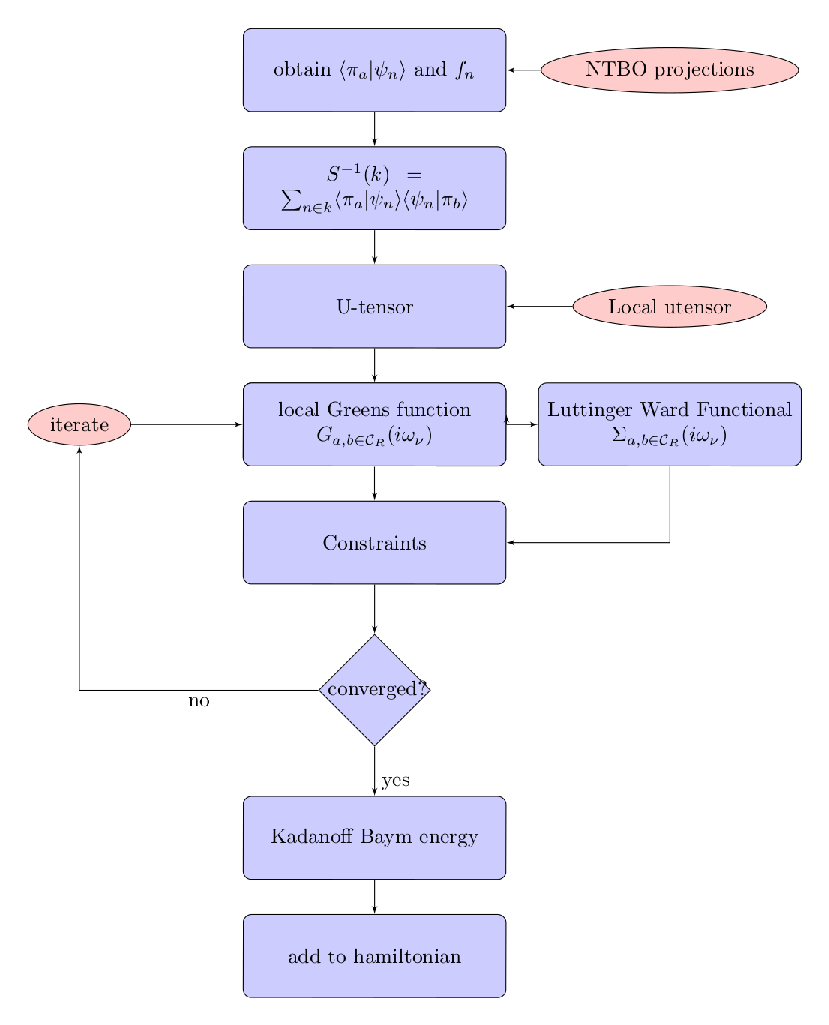
\includegraphics[width=0.5\linewidth]
{Figs/TikZ/FlowdiagramDMFTinterface/flow.eps}
\end{center}

%====================================================================
\subsection{DMFT\$GREEN}
%====================================================================
DMFT\$GREEN is the main subroutine of the DMFT object. It is called
from the LMTO object, which also provides the  projections onto the
tight-binding orbitals.

We evaluate the functional $Q^{\hat{W}_2}_{dyn,\beta}[\mat{\rho}]$
following the recipy provided in section III of the BPP
paper\cite{bloechl13_prb88_25139}.

\begin{verbatim}
call dmft_ini()
call dmft_collectnatorb()  
call dmft_rhoofk()  
call dmft_utensor() 
call dmft_natorb()
call dmft_hrho()
call dmft_constraints()
do iter=1,3
  call dmft_gloc() 
  call dmft_solver(etot) 
  call dmft_constraints()
enddo ! end of loop over iterations to enforce constraint
call dmft_rholocal()
call dmft_staticsolver(svar) 
etot=etot+svar
call dmft_detot(svar)
etot=etot+svar      
call energylist$set('dmft interface',etot)
call energylist$add('local correlation',etot)
call energylist$add('total energy',etot)
call dmft_addtohpsi()
\end{verbatim}

\begin{enumerate}
\item \verb|DMFT_COLLECTNATORB|: The orbital coefficients
  $\langle\pi_a|\psi_n\rangle$ have been calculated by the LMTO object
  and they are kept in the module of \verb|paw_waves|.  The orbital
  coefficients are placed into as 
  \verb|kset(ik)%pipsi(ndim,nchi,nb,nspin)|. Also the occupations are
  kept as \verb|kset(ik)%f(nb,nspin)| (without spin degeneracy,
  i.e. $f_n\in[0,1]$). The k-point weights are kept
  as \verb|kset(ik)%wkpt|. Again the spin degeneracy has been
  removed. However special k-points have half the weight as general
  k-points. \petertt{This should be checked explicitely!}
%
\item \verb|DMFT_rhoofk|: calculate the k-dependent density matrix,
  the inverse overlap matrix and the overlap matrix itself.
\begin{eqnarray}
\rho_{a,b}(\vec{k})&=&\sum_n
\langle\pi_a|\psi_n(\vec{k})\rangle f_n(\vec{k})
\langle\psi_n(\vec{k})|\pi_b\rangle
\\
\mat{S}^{-1}_{a,b}(\vec{k})&=&\sum_n
\langle\pi_a|\psi_n(\vec{k})\rangle 
\langle\psi_n(\vec{k})|\pi_b\rangle
\\
\mat{S}&=&\Bigl(\mat{S}^{-1}\Bigr)^{-1}
\end{eqnarray}
The k-dependent density matrix is kept as
\verb|kset(ik)%rho(nchi,nchi,ndimd)|. The inverse overlap matrix is
kept as \verb|kset(ik)%sinv(nchi,nchi,ndimd)| and the overlap matrix
is kept as \verb|kset(ik)%smat(nchi,nchi,ndimd)|.
%
\item \verb|DMFT_UTENSOR|: (see also
  section~\ref{sec:routinedmftutensor}) The local U-tensor is
  collected from the on-site elements \verb|POTPAR(ISP)%TAILED%U|
  calculated in the \verb|paw_LMTO| object. It is directly converted
  from the ``tailed representation'' into the basis of local orbitals.
\begin{eqnarray}
U_{a,b,c,d}=\alpha\int d^4x\int d^4x'\;
\frac{e^2\chi^*_a(\vec{x})\chi^*_b(\vec{x'})\chi_c(\vec{x})\chi_d(\vec{x'})}
{4\pi\epsilon_0|\vec{r}-\vec{r'}|}
\label{eq:defutensordmftobject}
\end{eqnarray}
Only the U-tensor for equal spin-electrons is stored. $\alpha$ is a
scale factor that mimics the screening of the U-tensor. It is called
\verb|LHFWEIGHT|.

The scaled U-tensor is kept as \verb|ATOMSET(iat)%U|
%
%=========================hrho========================================
\item \verb|DMFT_HRHO|: (see also section~\ref{sec:routinedmfthrho} on
p.~\pageref{sec:routinedmfthrho}.) Calculate the non-interacting
Hamiltonian $\bar{\mat{h}}_{\vec{k}}$ that produces the specified
(k-dependent) density matrix.
\begin{eqnarray}
\bar{h}_{\vec{k},a,b}=\mu S_{\vec{k},a,b}+\sum_{n}
\langle\chi_a|\psi'_{\vec{k},n}\rangle\frac{1}{\beta}
\ln\left[\frac{1-f'_{\vec{k},n}}{f'_{\vec{k},n}}\right]
\langle\psi'_{\vec{k},n}|\chi_b\rangle
\end{eqnarray}

$\bar{\mat{h}}_{\vec{k}}$ is kept as \verb|KSET(IKPT)%HRHO|.
%
%===============natorb=================================================
\item \verb|DMFT_NATORB|: (see also
  section~\ref{sec:routinedmftnatorb}) Despite the name we do no more
  use local natural orbitals. This is described in
  section~\ref{sec:routinedmftnatorb}. A this point we have three
  different settings for the routine \verb|DMFT_NATORB|: ``NATORB'',
  ``QUAMBO'' and ``ORTHO''. QUAMBO stands for ``quasi atomic molecular
  orbitals''\cite{qian08_prb78_245112}, while it may or may not be
  related to it.

  Construct the eigenstates $|\phi_j\rangle$ of the single-site
   matrix $\mat{A}$
\begin{eqnarray}
\hat{A}_R|\phi_{R,i}\rangle=|\phi_{R,i}\rangle a_{R,i}
\end{eqnarray}
These states will be called local natural orbitals (This will be
changed.).

The orbital coefficients $\langle\pi_a|\phi_{R,j}\rangle$ of the local
orthonormal orbitals are calculated as
\footnote{The spirit follows from the construction of local natural
  orbitals along the following lines
\begin{eqnarray}
\underbrace{\sum_{a,b}|\chi_a\rangle\langle\pi_a|\hat{A}_R|\pi_b\rangle
\langle\chi_b|}_{\hat{\rho}_R}
\underbrace{\sum_c|\chi_c\rangle x_{c,j}}_{|\phi_{R,j}\rangle}
=\underbrace{\sum_a|\chi_a\rangle x_{a,j}}_{|\phi_{R,j}\rangle} f'_{R,j}
\nonumber\\
\sum_{b,c}\langle\pi_a|\hat{\rho}_R|\pi_b\rangle
\langle\chi_b|\chi_c\rangle x_{c,j}
=x_{a,j}f'_{R,j}
\end{eqnarray}
Now, introduce $y_{a,j}=\sum_b\langle\chi_a|\chi_b\rangle x_{b,j}$
\begin{eqnarray}
\sum_{b}\langle\pi_a|\hat{\rho}_R|\pi_b\rangle y_{b,j}
=\sum_b S^{-1}_{a,b}y_{b,j}f'_{R,j}
\end{eqnarray}
which is a generalized eigenvalue problem for the vectors $\vec{y}_j$,
which are converted into orbital coefficients by multiplication with
$\mat{S}^{-1}$.
\begin{eqnarray}
|\phi_{R,j}\rangle=\sum_{a,b}|\chi_a\rangle S^{-1}_{a,b} y_{b,j}
\end{eqnarray}
The local natural orbitals are orthonormal in the sense
\begin{eqnarray}
\langle\phi_{R,i}|\phi_{R,j}\rangle
=\sum_{a,b,c,d}
y^*_{a,i}S^{-1}_{a,c}
\underbrace{\langle\chi_c|\chi_d\rangle}_{(\mat{S}^{-1})^{-1}}
 S^{-1}_{d,b} y_{b,j}
=\sum_{a,b}y^*_{a,i}S^{-1}_{a,b}y_{b,j}=\delta_{i,j}
\end{eqnarray}
}
\begin{eqnarray}
\sum_{b}\langle\pi_a|\hat{\rho}_R|\pi_b\rangle y_{b,j}
&=&\sum_b S^{-1}_{R,a,b}y_{b,j}f'_{R,j}
\qquad\text{with $\vec{y}^\dagger_i \mat{S}^{-1}_R\vec{y}_{j}=\delta_{i,j}$}
\\
\langle\pi_a|\phi_{R,j}\rangle&=&\sum_{b} S^{-1}_{R,a,b} y_{b,j}
\end{eqnarray}

The local density matrix $\mat{\rho}_R$ and the local inverse overlap
matrix $\mat{S}^{-1}_R$ are obtained as Brillouin zone intergral
projected onto the lcoal site
\begin{eqnarray}
\mat{\rho}_R&=&\mat{P}_R\Bigl[
\sum_{\vec{k}} w_{\vec{k}}\mat{\rho}(\vec{k})
\Bigr]\mat{P}_R
\nonumber\\
\mat{S}^{-1}_R&=&\mat{P}_R\Bigl[
\sum_{\vec{k}} w_{\vec{k}}\mat{S}^{-1}(\vec{k})
\Bigr]\mat{P}_R
\end{eqnarray}

The transformation matrices are stored in the fully non-collinear data
model in \verb|atomset%natorb%piphi| and the vectors $\vec{y}_j$ are
stored as \verb|atomset%natorb%chiphi|.

\petertt{The vector $y$ is used for the transformation to the local
  natural orbitals in the solver interface. Check if this is
  correct. should it be the vector $x$?}
%
%
\item \verb|DMFT_GLOC|: The local Green's function is obtained as
  Brillouin zone integral over the k-dependent greens function after
  projecting onto the correlated orbitals on the specified site.
\begin{eqnarray}
\mat{G}_R(i\omega_\nu)=\sum_k w_{\vec{k}}
\Bigl[(i\omega_\nu+\mu)\mat{S}_{\vec{k}}-
\bar{\mat{h}}_{\vec{k}}+\mat{\Gamma}_{\vec{k}}
-\mat{\Sigma}^{\hat{W}_2}_{dyn}(i\omega_\nu)\Bigr]^{-1}_R
\end{eqnarray}
The Laurent expansion is obtained as
\begin{eqnarray}
\mathcal{\mat{G}}^{(1)}_R(i\omega_\nu)&=&\sum_k w_{\vec{k}}
\mat{S}^{-1}_{\vec{k}}
\nonumber\\
\mathcal{\mat{G}}^{(2)}_R(i\omega_\nu)&=&\sum_k w_{\vec{k}}
\mat{S}^{-1}_{\vec{k}}
\Bigl(\bar{\mat{h}}-\mu\mat{S}_{\vec{k}}
+\mat{\Gamma}_{\vec{k}}-\mathcal{\mat{S}}_{dyn}^{(0)}\Bigr)
\mat{S}^{-1}_{\vec{k}}
\end{eqnarray}

The result and its Laurent expansion terms are stored in
\verb|atomset%gloc| and \verb|atomset%gloclaur|.
%
\item \verb|DMFT_SOLVER|: Calculates the dynamic contribution
  $\Phi^{LW,\hat{W}_2}_\beta-\Phi^{HF,\hat{W}_2}_\beta$ to the
  Luttinger-Ward functional and the corresponding contribution
  $\mat{\Sigma}_{dyn}^{\hat{W}_2}$ to the self energy for the
  specified Green's function.

  \begin{enumerate}
    \item In a first loop over atoms the atoms are individually
      adressed and the routine \verb|dmft_dynamicsolver| is
      called. 
    \item Inside \verb|dmft_dynamicsolver| the U-tensor and the
      Green's function are converted into local natural orbitals and
      in a up-down spinor representation with all up-spin components
      first and the down-spin components second.
    \item then the actual interface routine \verb|DMFT_SOLVERIO| is
      called, which returns the value of the dynamic contribution to
      the Luttinger-Ward functional (HF subtracted), the coresponding
      contribution to the self energy and the derivative of the
      U-tensor.
      \begin{eqnarray}
      \Phi^{LW}_{dyn}[\mat{G}(i\omega_\nu),\hat{W}_2]&=&
      \Phi^{LW}[\mat{G}(i\omega_\nu),\hat{W}_2] -\frac{1}{2}
      \sum_{a,b,c,d} U^{\hat{W}_2}_{a,b,d,c} \Bigl(
      \rho_{d,a}\rho_{c,b} - \rho_{c,a}\rho_{d,b}\Bigr) \Bigr) 
      \nonumber\\\
      \Sigma^{\hat{W}_2}_{dyn,a,b}(i\omega_\nu)&=&
      \frac{\beta\partial\Phi^{LW}}{\partial G_{b,a}(i\omega_\nu)}
      -\sum_{c,d}\Bigl(U^{\hat{W}_2}_{a,c,b,d}-U^{\hat{W}_2}_{a,c,d,b}\Bigr)
      \rho_{d,c}
      \nonumber\\
      \mathcal{\mat{S}}^{(0)}_{dyn,a,b}
       &=&\frac{1}{\beta}\sum_{|\nu|>\nu_x}
       \frac{1}{(i\hbar\omega_\nu)^2}\biggl[
       \frac{\beta\partial\Phi^{LW}}{\partial G_{b,a}(i\omega_\nu)}
      -\sum_{c,d}\Bigl(U^{\hat{W}_2}_{a,c,b,d}-U^{\hat{W}_2}_{a,c,d,b}\Bigr)
      \rho_{d,c}\biggr]
      \nonumber\\
      %
      \frac{\delta\Phi^{dyn,LW}_\beta}{\delta U_{a,b,c,d}}&=&
      \frac{\delta\Phi^{LW}_\beta}{\delta U_{a,b,d,c}}
      -\frac{1}{2}\Bigl(
      \rho_{d,a}\rho_{c,b} - \rho_{c,a}\rho_{d,b}\Bigr) \Bigr) 
      \end{eqnarray}
      \petertt{pay attention to the reversed order of the indices
        $c,d$!}  

       $\frac{\delta\Phi^{dyn,LW}_\beta}{\delta U_{a,b,c,d}}$ is the
      difference of the two-particle density for the interacting and
      the non-interacting electron gas at the same density matrix. In
      contrast to the corresponding term in the density functional
      theory, this term does not contain a kinetic energy contribution
      as does $n(\vec{r})\int_0^1 d\lambda\;
        h_{\lambda}(\vec{r},\vec{r'})$, but rather
        $n(\vec{r})\Bigl[h_{1}(\vec{r},\vec{r'})
          -h_{0}(\vec{r},\vec{r'})\Bigr]$
    %
    \item After \verb|DMFT_SOLVERIO| is finished, the self energy and
      the derivative with respect to the U-tensor are transformed
      back.
  \end{enumerate}
  The external solver may make additional approximations to the
  U-tensor or to the Kadanoff-Baym functional. However, these
  approximations must be consistent across the dynamical-correlation
  correction.
%
\item \verb|DMFT_MIX| mixes the self energy: The self energy cannot
  simply be inserted into the Green's function for the next iteration,
  because the changes for small Matsubara frequencies would be too
  violent. Therefore, it needs some preconditioning.

  The underlying ideas related to the mixing are described in
  appendix~\ref{sec:mixing} on p.~\pageref{sec:mixing}.
  \begin{eqnarray}
    \Sigma^{dyn}_{a,b}(i\omega_\nu)
&\leftarrow&\Sigma^{dyn}_{a,b}(i\omega_\nu)
+\frac{1}{C}\Bigl(\frac{C}{M}+(\hbar\omega)^2\Bigr)
\biggl(\Sigma^{dyn}_{a,b}(i\omega_\nu)
-\frac{\beta\delta\Phi^{LW}_{dyn}}{\partial G_{b,a}(i\omega_\nu)}
\biggr)
\nonumber\\
   \mathcal{\mat{S}}_{dyn,a,b}^{(0)}&\leftarrow&\mathcal{\mat{S}}_{dyn,a,b}^{(0)}
+\frac{(\hbar\omega_x)^2}{C}\biggl(\mathcal{\mat{S}}_{dyn,a,b}^{(0)}
-\frac{\delta\Phi^{LW}_{dyn}}{\delta\mathcal{G}^{(2)}_{b,a}}\biggr)
\end{eqnarray}
\petertt{It seems that the sign for the mixing is incorrect!! I am
  changing it in the code to see what happens.}  $\mat{\Sigma}^{dyn}$
is the self energy that has been accumulated, and that is zero in the
first iteration. $\frac{\beta\delta\Phi^{LW}_{dyn}} {\partial
  G_{b,a}(i\omega_\nu)}$ is the dynamic self-energy contribution
produced by the solver. Note that this self energy does not contain
the Hartree-Fock term. $C$ and $M$ are two mixing parameters, that
control the behavior at small ($M$) and large ($C$) Matsubara
frequencies.
%
\item \verb|DMFT_CONSTRAINTS| enforced the density matrix constraint:
  The new Green's function $\mat{G}^{new}$ has the form
\begin{eqnarray}
\mat{G}^{new}(i\omega_\nu)=\Bigl[(i\hbar\omega_\nu+\mu)\mat{1}
-\bar{\mat{h}}+\mat{\Gamma}
-\mat{\Sigma}^{dyn}(i\omega_\nu)
\Bigr]^{-1}
\end{eqnarray}
where the Lagrange multiplier $\mat{\Gamma}$ needs to be adjusted until
the density matrix constraint
\begin{eqnarray}
\mat{\rho}=\frac{1}{\beta}\sum_\nu 
\e{i\beta\hbar\omega_\nu0^+}\mat{G}^{new}(i\omega_\nu)
\end{eqnarray}
is fulfilled. 

For this purpose, we linearize the constraint equation in the Lagrange
multiplier
\begin{eqnarray}
\mat{\rho}&=&\frac{1}{\beta}\sum_\nu 
\e{i\beta\hbar\omega_\nu0^+}
\biggl[
\mat{G}^{new}(i\omega_\nu)-\mat{G}^{new}(i\omega_\nu)\delta\mat{\Gamma}
\mat{G}^{new}(i\omega_\nu)\biggr]
\nonumber\\
0&=&\left[\frac{1}{\beta}\sum_\nu \e{i\beta\hbar\omega_\nu0^+}
G^{new}_{a,b}(i\omega_\nu)\right]-\rho_{a,b}
-\sum_{c,d}\left[
\frac{1}{\beta}\sum_\nu 
\mat{G}^{new}_{a,c}(i\omega_\nu)\mat{G}^{new}_{d,b}(i\omega_\nu)\right]
\delta\mat{\Gamma}_{c,d}
\nonumber\\
\delta\mat{\Gamma}_{c,d}
&=&
\underbrace{
\left[
\frac{1}{\beta}\sum_\nu 
\mat{G}^{new}_{a,c}(i\omega_\nu)\mat{G}^{new}_{d,b}(i\omega_\nu)
\right]^{-1}_{cd,ab}
}_{\leadsto\quad \alpha\delta_{c,a}\delta_{d,b}}
\biggl(
\underbrace{\left[\frac{1}{\beta}\sum_\nu \e{i\beta\hbar\omega_\nu0^+}
G^{new}_{a,b}(i\omega_\nu)\right]}_{\rho^{new}_{a,b}}-\rho_{a,b}
\biggr)
\end{eqnarray}
\petertt{In this equation we can use the model Green's function to
  avoid the calculation and inversion of
  $\mat{G}^{new}\otimes\mat{G}^{new}$}

Note, that $\mat{\Gamma}$ is, like $\mat{h'}$, a non-local Hamiltonian,
that in principle connects arbitrary local orbitals with each
other. In a Bloch representation, $\mat{\Gamma}$ is a k-dependent matrix,
which connects all local orbitals in the unit cell with each other.

Thus, we iterate the coupled equations
\begin{eqnarray}
\mat{G}^{new}(i\omega_\nu)&=&\Bigl[(i\hbar\omega_\nu+\mu)\mat{1}
-\bar{\mat{h}}+\mat{\Gamma}
-\mat{\Sigma}^{dyn}(i\omega_\nu)
\Bigr]^{-1}
\nonumber\\
\delta\mat{\rho}&=&\frac{1}{\beta}\sum_\nu 
\e{i\beta\hbar\omega_\nu0^+}\mat{G}^{new}(i\omega_\nu)-\mat{\rho}
\nonumber\\
\mat{\Gamma}&=&\mat{\Gamma}+\alpha \delta\mat{\rho}
\end{eqnarray}
until $\delta\rho$ vanishes.

\petertt{In practice we do not use $\alpha$, but precondition with a
  Green's function with zero one-particle level. see
  section~\ref{sec:routinedmftconstraints}.}

With the correct Lagrange multiplier, the new Green's function is
obtained.
%
\item \verb|DMFT_RHOLOCAL|: For the Hartree-Fock and DFT
  double-counting terms, we need the local density matrix, which is
  calculatecd directly form the k-dependent density matrix als
  Brillouin zone sum.
%
\item \verb|DMFT_STATICSOLVER|: Calculates the static contribution to
  the correlation energy, i.e. the screened Hartree-Fock term and the
  DFT double counting correction and its derivatives. These terms do
  not affect the density matrix constraint.

   \petertt{This term must be removed if the corresponding terms are
     treated in the PAW\_LMTO object. The double counting for the
     correlation must however still be included.}

    \petertt{For the double counting in the HF approximation, only the
      exchange part is removed, while, here, also the correlation
      contribution should be taken out, because the correlation is
      explicitly added.}

    The Hartree-Fock contribution is added directly to the double
  counting term. Thus the self energy \verb|atomset%sigma| is only
  the dynamical contribution.
%
\item \verb|DMFT_DETOT|: Adds the non-local contribution to the total energy
\begin{eqnarray}
&-&\frac{1}{\beta}\sum_\nu\Tr\Bigl\lbrace
\ln\Bigl[
\mat{1}-
\Bigl(i\hbar\omega_\nu+\mu)\mat{1}-\bar{\mat{h}}\Bigr)^{-1}
\Bigl(
\mat{\Sigma}^{\hat{W}_2}_{dyn}(i\omega_\nu)-\mat{\Gamma}\Bigr)
\Bigr]
\nonumber\\&&
+\Bigl(\mat{\Sigma}^{\hat{W}_2}_{dyn}(i\omega_\nu)
-\mat{\Gamma}\Bigr)\mat{G}(i\omega_\nu)
+
\Bigl[
\mat{G}(i\omega_\nu)
-\Bigl(i\hbar\omega_\nu+\mu)\mat{1}-\bar{\mat{h}}\Bigr)^{-1}
\Bigr[
\mat{\Gamma}\Bigr\rbrace
\end{eqnarray}

In order to evaluate the logarithm, I diagonalize the non-hermitean
matrix in the argument, and sum the absolute values of the
eigenvalues. The complex logarithm is $\ln[z]=\ln(|z|)+i Arg(z)$. The
imaginary part cancels out with the negative Matsubara frequencies.

\petertt{In a previous version I used the Dahlen trick, which is
  probably not quite correct. See appendix~\ref{sec:dahlenstrick} on
  p.~\pageref{sec:dahlenstrick} }
%
\item \verb|DMFT_ADDTOHPSI|: Adds the energy derivative to
  \verb|this%htbc| of the \verb|waves_module|. There are two
  contributions, a k-dependent term which is restricted to the
  correlated orbitals and an site-dependent term that acts on all
  local orbitals.
\begin{itemize}
\item The site-specific term contains the double counting term for the
  DFT functional and the Hartree-Fock contribution to the self energy.
\end{itemize}
\end{enumerate}



%====================================================================
\subsection{DMFT\_INI}
%====================================================================

%====================================================================
\subsubsection{Hardwired data}
%====================================================================
\begin{itemize}
\item NOMEGA ($N_\omega$)
\end{itemize}

%====================================================================
\subsubsection{Inherited data}
%====================================================================
\begin{itemize}
\item NDIM from \verb|waves_module|
\item NSPIN from \verb|waves_module|
\item NKPTL from \verb|waves_module|
\item NAT  from \verb|ATOMLIST| Object
\item isp(IAT)
\item WKPT and (NKPT,KMAP) from \verb|DYNOCC| Object
\item KBT from \verb|dynocc$getr8a('temp')| from
  \verb|paw_occupations.f90|
\item \verb|atomset(iat)%lhfweight| from \verb|lmto_module|
\end{itemize}

%====================================================================
\subsubsection{Derived data}
%====================================================================
\begin{itemize}
\item NDIMD (=1 for NDIM=1,NSPIN=1; =2 for NDIM=1,NSPIN=2; =4 for
  NDIM=2,NSPIN=1)
\item List of positive Matsubara frequencies
\begin{eqnarray}
\omega_\nu=(2\nu-1)\pi k_BT \qquad\text{for $\nu=1,\ldots,N_\omega$}
\end{eqnarray}
\item Atomset structure
\begin{center}
 \begin{tabular}{ll}
 \verb|atomset\%nloc| & number of correlated orbits on this atom \\
\verb|atomset\%ICHI1| & first value of ICHI index for this atom\\
\verb|atomset\%ICHI2| & last value of ICHI index for this atom\\
\end{tabular}
\end{center}
%
\item KSET structure
\begin{center}
 \begin{tabular}{ll}
 \verb|KSET\%WKPT| & geometric k-point weight\\
\end{tabular}
\end{center}
\end{itemize}

%====================================================================
\subsection{DMFT\_UTENSOR}
\label{sec:routinedmftutensor}
%====================================================================
Obtain the on-site U-tensor\index{U-tensor} for all local orbitals from
subroutine \verb|dmft_ulocal| reduces it to the entries for the
correlated orbitals.

In \verb|DMFT_ULOCAL| it obtains the local U-tensor from the
\verb|POTPAR%TAILED%U| and \verb|SBAR| of the LMTO Object. This object
contains the extended $\phi$ and $\dot{\phi}$ functions
\begin{eqnarray}
|\chi_a\rangle=|\phi_a\rangle-
\sum_{b; R_b=R_a}|\dot{\bar{\phi}}_b\rangle \bar{S}_{a,b}
\end{eqnarray}


The U-tensor is constructed in \verb|LMTO_MAKETAILEDPARTIALWAVES|.
\verb|LMTO_ULITTLE| constructs
\begin{eqnarray}
u_{\ell,a,b,c,d}
=\frac{2\ell+1}{4\pi}
\int dr\; r^2R_c(r)R_d(r)\Bigl[\int d^3r'\;V_\ell(r,r')R_a(r')R_b(r')\Bigr]
\end{eqnarray}
where the kernel $V_\ell(r,r')$ is the one used by \verb|RADIAL$POISSON|.
\textbf{There is a input parameter that determines which $\ell$ values are
considered.}

In \verb|LMTO_UTENSOR| the U-tensor elements are composed according to
\begin{eqnarray}
U_{a,b,c,d}=\sum_{ell}\frac{4\pi}{2\ell+1}\sum_{m=-\ell}^\ell
u_{\ell,b,d,c,a} C_{L,L_b,L_d}C_{L,L_c,L_a}
\end{eqnarray}

The U-tensor is screened by a factor \verb|LHFWEIGHT|. It is obtained
from the \verb|lmto_module| either as the global value \verb|HFWEIGHT|
or the individual value from hybridsetting. This very same factor is
used for the double counting term.

Thus the U-tensor is defined as\footnote{$\vec{x}=(\vec{r},\sigma)$}
in Eq.~\ref{eq:defutensordmftobject}, i.e. as
\begin{eqnarray}
U_{a,b,c,d}=\int d^4x\int d^4x'\;
\frac{e^2\chi^*_a(\vec{x})\chi^*_b(\vec{x'})\chi_c(\vec{x})\chi_d(\vec{x'})}
{4\pi\epsilon_0|\vec{r}-\vec{r'}|}
\end{eqnarray}
The U-tensor contributes only if $\sigma_a=\sigma_c$ and if
$\sigma_b=\sigma_d$.
With this definition the Hartree and exchange  energy have the form
\begin{eqnarray}
E_H=\frac{1}{2}\sum_{a,b,c,d}U_{a,b,c,d}\;\rho_{c,a}\rho_{d,b}
\nonumber\\
E_X=\frac{1}{2}\sum_{a,b,c,d}U_{a,b,c,d}\;\rho_{c,b}\rho_{d,a}
\end{eqnarray}


%====================================================================
\subsection{DMFT\_NATORB}
\label{sec:routinedmftnatorb}
%====================================================================
Construct a set of orthonormal states for the single-site problem.
This section describes first the mapping to local natural
orbitals. Later we will propose a different basisset, which avoids
some of the problems.

For this purpose, I redefine the unity operator for the sub Hilbert
space of correlated orbitals.
\begin{eqnarray}
\hat{1}_{\mathcal{C}_R}
=\sum_{\alpha,\beta}\sum_n
|\chi_\alpha\rangle
\langle\pi_\alpha|\psi_n\rangle\langle\psi_n|\pi_\beta\rangle
\langle\chi_\beta|
\end{eqnarray}
which allows one to identify the inverse overlap matrix in this
sub-Hilbert space.
\begin{eqnarray}
\mat{S}^{-1}_{\alpha,\beta}
=\sum_{\alpha,\beta}\sum_n
\langle\pi_\alpha|\psi_n\rangle\langle\psi_n|\pi_\beta\rangle
\end{eqnarray}
Note,however, that this matrix lives only on a single site! We can
obtain it from the k-dependent $\mat{S}^{-1}$ by summing over k-points
and cutting out the corresponding submatrix. However, it is not
allowed to do the same thing for the overlap matrix itself!

We approach the problem by a formulation of natural orbitals for the
local density matrix. This choice is not convenient in the end,
because the resulting basisset depends on the instantaneous electronic
structure. Nevertheless the point of view taken allows me to formulate
the problem. Later we change it such that we use quasi atomic orbitals
instead of the natural orbitals, which are less dependent on the
electronic structure.

The one-particle density matrix in this sub-Hilbert space has the form
\begin{eqnarray}
\hat{\rho}_{\mathcal{C}_R}
=\sum_{\alpha,\beta}\sum_n
|\chi_\alpha\rangle
\langle\pi_\alpha|\psi_n\rangle f_n \langle\psi_n|\pi_\beta\rangle
\langle\chi_\beta|
\end{eqnarray}

The eigenvalue equation
\begin{eqnarray}
\hat{\rho}|\phi_n\rangle&=&|\phi_n\rangle f_n
\nonumber\\
\sum_{\alpha,\beta}|\chi_\alpha\rangle
\langle\pi_\alpha|\hat{\rho}|\pi_\beta\rangle\langle\chi_\beta|\phi_j\rangle
&=&\sum_{\alpha,\beta}|\chi_\alpha\rangle\langle\pi_\alpha|\pi_\beta\rangle
\langle\chi_\beta|\phi_j\rangle f_j
=\sum_{\alpha,\beta}|\chi_\alpha\rangle
\mat{S}^{-1}_{\alpha,\beta}\langle\chi_\beta|\phi_j\rangle \bar{f}_j
\end{eqnarray}
provides us with a new set of occupations $\bar{f}$ of local natural
orbitals and eigenvectors
$\langle\chi_\beta|\phi_j\rangle=V_{\beta,j}$.
\begin{eqnarray}
\mat{\rho}\mat{V}=\mat{S}^{-1}\mat{V}\bar{f}
\qquad\text{with}\qquad
\mat{V}^\dagger\mat{S}^{-1}\mat{V}=\mat{1}
\label{eq:eigenvaluprobforlocalnatorb}
\end{eqnarray}

The natural orbitals are
\begin{eqnarray}
|\phi_j\rangle=\sum_{\alpha,\beta\in\mathcal{C}_R}
\underbrace{|\chi_\alpha\rangle
\mat{S}^{-1}_{\alpha,\beta}\langle\chi_\beta|}_{\mat{1}_{\mathcal{C}_R}}
\phi_j\rangle
=\sum_{\alpha\in\mathcal{C}_R}|\chi_\alpha\rangle
\underbrace{\Bigl(\mat{S}^{-1}\mat{V}\Bigr)_{\alpha,j}}_{\mat{V}^{\dagger,-1}_{\alpha,j}}
\end{eqnarray}
Remember that the natural orbitals are not the ones used in the
calculation! The orbitals chosen are discussed in the following
section.


The matrix $\mat{V}$ is placed into the structure
\verb|atomset%natorb%chiphi|, together with the occupations $\bar{f}$
which are in \verb|atomset%natorb%f|. In addition we store
$\mat{S}^{-1}\mat{V}=\mat{V}^{\dagger,-1}$ in
\verb|atomset%natorb%piphi| All data in \verb|atomset%natorb| are
stored in the fully non-collinear model.

%====================================================================
\subsubsection{Orthonormal orbitals without reference to the density matrix}
%====================================================================
When approximations are done on the U-tensor, which are not invariant
under a unitary transformation of the orbitals, the resulting U-tensor
will be itself a functional of the natural orbitals. The approximation
of a constant U-tensor in the solver will then lead to uncontrolled
results.

For this reason we choose an alternative basisset instead of the local
natural orbitals. The main requirement for the basisset is that it is
orthonormal.  Orthonormality can be obtained from any eigenvalue
problem of the form
\begin{eqnarray}
\mat{A}\mat{V}=\mat{S}^{-1}\mat{V}\mat{a}
\end{eqnarray}
where $\mat{A}$ is an arbitrary hermitean matrix, the the matrix
$\mat{V}$ containes the eigenvectors, which obey
$\mat{V}^\dagger\mat{S}^{-1}\mat{V}=\mat{1}$ and the diagonal matrix
$\mat{a}$ containes the eigenvalues of $\mat{A}$.

This eigenvalue equation replaces \eq{eq:eigenvaluprobforlocalnatorb}.

As a second criterion, we choose orbitals that closely reflect the
shape of the original tight-binding orbitals. In the current
implementation the tight-binding orbitals are constructed with a clear
main angular momentum character. \petertt{If the approximations made
  by the solver on the U-tensor are not rotationally invariant, one
  should use here a coordinate system that adapts to the changing
  local environment.}

If one chooses the matrix $\mat{A}$ to be diagonal, with very
different diagonal elements, then the eigenstates will be
correspondingly similar to the original orbitals, and they will remain
in the original order if the diagonal elements increase with index
number.

Therefore, I choose $A_{i,j}=j\delta_{i,j}$. A scale factor is
redundant, because it only affects the eigenvalues, but not the
eigenvectors.


%====================================================================
\subsection{DMFT\_HRHO}
\label{sec:routinedmfthrho}
%====================================================================
Calculate the non-interacting Hamiltonian $\bar{\mat{h}}$ that
produces the specified (k-dependent) density matrix.
\begin{eqnarray}
\bar{h}_{a,b}(\vec{k})=\mu S_{a,b}(\vec{k})+\sum_n\langle\chi_a|\psi_n'\rangle
\frac{1}{\beta}\ln\left[\frac{1-f'_n}{f'_n}\right]
\langle\psi'_n|\chi_b\rangle
\end{eqnarray}
where the natural orbitals $|\psi'_n\rangle$ and the occupations
$f'_n$ differ from the original natural orbitals.

\begin{enumerate}
  \item First, we transform onto natural orbitals 
     \begin{eqnarray}
        |\psi'_n\rangle=\sum_a|\chi_a\rangle \langle\pi_a|\psi'_n\rangle
     \end{eqnarray}
     These natural orbitals may be slighly different from the original
     natural orbitals, because they are restricted to the space of
     local orbitals.
     \begin{eqnarray}
        \hat{\rho}|\psi'_n\rangle&=&|\psi'_n\rangle f'_n
        \nonumber\\
        \langle\chi_a|
        \underbrace{\sum_{b,c}|\chi_b\rangle
        \overbrace{
           \Bigl(\sum_m\langle\pi_b|\psi_m\rangle f_m
                 \langle\psi_m|\pi_c\rangle\Bigr)}^{\rho_{b,c}}
               \langle\chi_c|}_{\hat{\rho}}
             \underbrace{\sum_d|\chi_d\rangle\langle\pi_d|\psi'_n\rangle
              }_{|\psi'_n\rangle}
             &=&
             \langle\chi_a|
             \underbrace{\sum_d|\chi_d\rangle\langle\pi_d|\psi'_n\rangle
              }_{|\psi'_n\rangle} f'_n
     \nonumber\\
           S_{a,b}\rho_{b,c}S_{c,d}\langle\pi_d|\psi'_n\rangle
           &=&S_{a,d}\langle\pi_d|\psi'_n\rangle f'_n
     \nonumber\\
           \mat{\rho} \Bigl(\mat{S} \vec{x}_n\Bigr)
           &=&\mat{S}^{-1}\Bigl(\mat{S} \vec{x}_n\Bigr) f'_n
     \end{eqnarray}

     Thus, for each k-point solve the generalized eigenvalue problem
     \begin{eqnarray*}
        \mat{\rho}(k)\mat{V}(\vec{k})=
        \mat{S}^{-1}(\vec{k})\mat{V}(\vec{k})\mat{f}'(\vec{k})
     \end{eqnarray*}
     where $\mat{f}'(\vec{k})$ is a diagonal matrix that contains
     k-dependent occupations. (They differ from the occupations $f_n$
     of the natural orbitals $|\psi_n\rangle$.)
%
\item Next we evaluate the hamiltonian $\bar{\mat{h}}$ in the
  representation of the natural orbitals $|\psi'_n\rangle$.

  The conversion of occupations into energies is done in the routine
  \verb|DMFT_EOFF|, described in section~\ref{sec:dmfteoff}.
  \begin{eqnarray}
  \epsilon=\mu+k_B
  \begin{cases}
  \ln\left(\frac{1-f}{f}\right) &\text{for $f_0<f<1-f_0$}\\
  a+b(f-f_0)&\text{for $f<f_0$}\\
  -a+b(f-(1-f_0))&\text{for $f>1-f_0$}\\
  \end{cases}
  \end{eqnarray}
  where $a$ and $b$ are determined such that the mapping is
  differentiable. The value of $f_0$ is currently set to $10^{-6}$.

  The energies obtained from \verb|DMFT_EOFF| are still spread over a
  too large energy interval. Therefore, we limit the energies to the
  interval $[\mu-zk_BT,\mu+zk_BT]$, where $z$ is a fixed
  parameter. $z$ should be chosen so that the occupations calculated
  with the Fermi distribution from $\bar{\mat{h}}$ are not affected
  too much.

\begin{center}
\begin{tabular}{|c|c|}
\hline
$z$ & $min(f); max(1-f)$ \\
\hline
$4.6$ & $10^{-2}$\\
$6.9$ & $10^{-3}$\\
$9.2$ & $10^{-4}$\\
$11.5$ & $10^{-5}$\\
$14.8$ & $10^{-6}$\\
\hline
\end{tabular}
\end{center}

\begin{figure}
\begin{center}
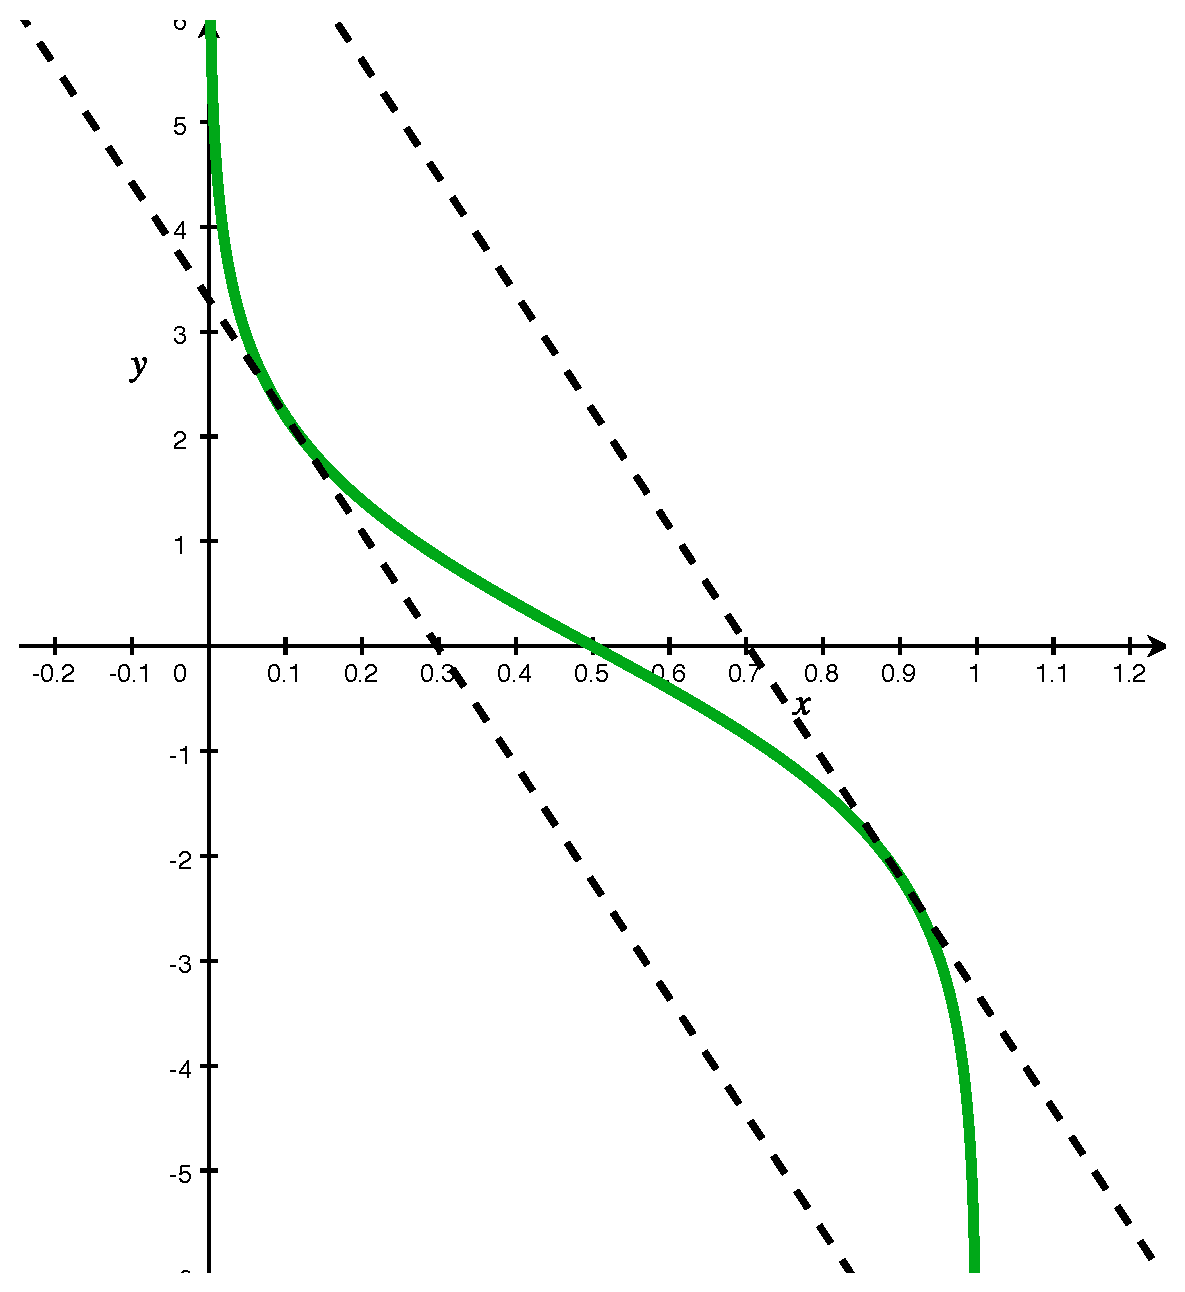
\includegraphics[width=0.5\linewidth]{Figs/Grapher/Eoff/eoff.eps}
\end{center}
\caption{\label{fig:eoff}Inverted Fermi function (green full line) and
  linear extensions (dashed) map occupations onto energies in
  DMFT\_EOFF. Here the extensions are at $f_0=0.1$ and $f_0=0.9$.}
\end{figure}


  


%
\item next we transform this Hamiltonian back into the basis of local
  orbitals, where the Hamniltonian has the form
  $\bar{h}_{a,b}=\langle\chi_a|\hat{\bar{h}}|\chi_b\rangle$,
  respectively $\hat{\bar{j}}=\sum_{a,b}|\pi_a\rangle
  h_{a,b}\langle\pi_b|$.
  \begin{eqnarray}
    \hat{\bar{h}}&=&\sum_n|\psi'_n\rangle\epsilon_n\langle\psi'_n|
  \nonumber\\
    \langle\chi_a|\hat{\bar{h}}|\chi_b\rangle&=&
    \sum_n\langle\chi_a|\psi'_n\rangle\epsilon_n\langle\psi'_n|\chi_b\rangle
   \nonumber\\
    &=&
    \sum_{n,c,d}\langle\chi_a|\chi_c\rangle\langle\pi_c|\psi'_n\rangle\epsilon_n
     \langle\psi'_n|\pi_d\rangle\langle\chi_d|\chi_b\rangle
    =V_{a,n}\epsilon_n V^\dagger_{n,b}
   \nonumber\\
     \bar{\mat{h}}(\vec{k})&=&
       \mat{V}\mat{\epsilon}\mat{V}^\dagger
   \end{eqnarray}
\end{enumerate}

%====================================================================
\subsubsection{DMFT\_EOFF}
\label{sec:dmfteoff}
%====================================================================
The routine \verb|DMFT\_EOFF| constructs the energy relative to the
Fermi level $x=\epsilon-\mu$ for a given occupation $f$. It modifies
the Fermi distribution in order to avoid infinities near $f=0$ and
$f=1$. Furthermore the modified mapping produces energies even for
occupations outside the interval $[0,1]$. The modification is to
extend the fermi functions linearly outside the interval
$[f_{min},1-f_{min}]$, where $f_{min}$ is a fixed parameter.

Let us first determine the inverted function of the Fermi distribution
and calculate its energies.
\begin{eqnarray}
f(x)&=&\left(1+\e{\beta x}\right)^{-1}
\quad\Rightarrow f+f\e{\beta x}=1
\quad\Rightarrow \e{\beta x}=\frac{1-f}{f}
\\
\Rightarrow\quad
x(f)&=&k_BT\ln\left(\frac{1-f}{f}\right)
\\
\Rightarrow\quad
\frac{dx}{df}&=&k_BT\frac{f}{1-f}\left[\frac{-1}{f}-\frac{1-f}{f^2}\right]
=k_BT\frac{f}{1-f}\left[\frac{-1}{f}-\frac{1-f}{f^2}\right]
\nonumber\\
&=&-k_BT\frac{1}{f(1-f)}
\end{eqnarray}

\begin{itemize}
\item for $f\in[f_{min},1-f_{min}]$ we evaluate
\begin{eqnarray}
  x(f)&=&k_BT\ln\left(\frac{1-f}{f}\right)
\end{eqnarray}
%
\item for $f$ outside the interval $f\in[f_{min},1-f_{min}]$, we choose
\begin{eqnarray}
f_0=\begin{cases}
f_{min}&\text{for $f\le f_{min}$}\\
1-f_{min}&\text{for $f\ge 1-f_{min}$}\\
\end{cases}
\end{eqnarray}
and determine 
\begin{eqnarray}
x(f)=x(f_0)+\left.\frac{dx}{df}\right|_{f_0}(f-f_0)
\end{eqnarray}
\end{itemize}
This construction produces a unique mapping from the occupations to
the energies $\epsilon=\mu+x$, even for occupations outside $[0,1]$.


%====================================================================
\subsection{DMFT\_CONSTRAINTS}
\label{sec:routinedmftconstraints}
%====================================================================
%====================================================================
\subsubsection{Green's function}
%====================================================================
The Green's function is calculated as follows
\begin{eqnarray}
\mat{G}(\vec{k},i\omega_\nu)&=&
\Bigl[
(i\omega_\nu+\mu)\mat{S}(\vec{k})-\bar{\mat{h}}(\vec{k})+\mat{\Gamma}(\vec{k})
-\sum_R\mat{\Sigma}^{dyn}_R(i\omega_\nu)
\Bigr]^{-1}
\end{eqnarray}
As described in section~\ref{sec:laurentgreen} on
p.~\pageref{sec:laurentgreen}, the Laurent-expansion coefficients are
\begin{eqnarray}
\mat{\mathcal{G}}^{(1)}(\vec{k})&=&\mat{S}^{-1}(\vec{k})
%
\nonumber\\
\mat{\mathcal{G}}^{(2)}(\vec{k})&=&\mat{S}^{-1}(\vec{k})
\Bigl(-\mu\mat{S}(\vec{k})+\bar{\mat{h}}(\vec{k})-\mat{\Gamma}(\vec{k})
+\mat{\mathcal{S}}^{(0)}_{dyn}(\vec{k})
\Bigr)
\mat{S}^{-1}(\vec{k})
%
\nonumber\\
\mat{\mathcal{G}}^{(3)}(\vec{k})&=&
\mat{S}^{-1}(\vec{k})
\biggl[
\mat{\mathcal{S}}^{(1)}_{dyn}(\vec{k})+
\Bigl(-\mu\mat{S}(\vec{k})+\bar{\mat{h}}(\vec{k})-\mat{\Gamma}(\vec{k})
+\mat{\mathcal{S}}^{(0)}_{dyn}(\vec{k})\Bigr)
\nonumber\\
&&\times\mat{S}^{-1}(\vec{k})
\Bigl(-\mu\mat{S}(\vec{k})+\bar{\mat{h}}(\vec{k})-\mat{\Gamma}(\vec{k})
+\mat{\mathcal{S}}^{(0)}_{dyn}(\vec{k})\Bigr)
\biggr]
\mat{S}^{-1}(\vec{k})
\nonumber\\
\end{eqnarray}
%
%====================================================================
\subsubsection{Green's function difference}
%====================================================================
In order to calculate the constraint, it may be adviseable to directly
evaluate the difference of te Green's function from the
non-interacting Greens function $\bar{\mat{G}}$.
\begin{eqnarray}
\Delta\mathcal{G}^{(1)}(\vec{k})&=&0
\nonumber\\
\Delta\mathcal{G}^{(2)}(\vec{k})&=&\mat{S}^{-1}(\vec{k})
\Bigl(
\mat{\mathcal{S}}^{(0)}_{dyn}(\vec{k})-\mat{\Gamma}(\vec{k})
\Bigr)
\mat{S}^{-1}(\vec{k})
%
\nonumber\\
\Delta\mat{\mathcal{G}}^{(3)}(\vec{k})
&=&
\mat{S}^{-1}(\vec{k})
\biggl[
\mat{\mathcal{S}}^{(1)}_{dyn}(\vec{k})+
\Bigl(-\mu\mat{S}(\vec{k})+\bar{\mat{h}}(\vec{k})-\mat{\Gamma}(\vec{k})
+\mat{\mathcal{S}}^{(0)}_{dyn}(\vec{k})\Bigr)
\nonumber\\
&&\times\mat{S}^{-1}(\vec{k})
\Bigl(-\mu\mat{S}(\vec{k})+\bar{\mat{h}}(\vec{k})-\mat{\Gamma}(\vec{k})
+\mat{\mathcal{S}}^{(0)}_{dyn}(\vec{k})\Bigr)
\nonumber\\
&&-
\Bigl(-\mu\mat{S}(\vec{k})+\bar{\mat{h}}(\vec{k})\Bigr)
\mat{S}^{-1}(\vec{k})
\Bigl(-\mu\mat{S}(\vec{k})+\bar{\mat{h}}(\vec{k})\Bigr)
\biggr]
\mat{S}^{-1}(\vec{k})
\end{eqnarray}

%============================================================================
\subsubsection{Update $\mat{\Gamma}$}
%============================================================================
\begin{myshadowminipage}{Update $\Gamma$}
The following two equations are solved iteratively\footnote{Instead of
  subtracting the density matrix from the Matsubara sum for the
  Green'sfunction, we subtract the Greens function $\bar{\mat{G}}$
  inside the Matsubara sum to avoid numerical problems due to the
  finite Matsubara sum.}
\begin{eqnarray}
\delta\mat{\rho}(\vec{k})&=&
\biggl(\frac{1}{\beta}\sum_\nu
\underbrace{\Bigl[
(i\omega_\nu+\mu)\mat{S}(\vec{k})-\bar{\mat{h}}(\vec{k})+\mat{\Gamma}(\vec{k})
-\sum_R\mat{\Sigma}^{dyn}_R(i\omega_\nu)
\Bigr]^{-1}}_{\mat{G}(\vec{k})}\biggr)
\nonumber]\\
&&\hspace{1cm}-\underbrace{\Bigl[
(i\omega_\nu+\mu)\mat{S}(\vec{k})-\bar{\mat{h}}(\vec{k})\Bigr]^{-1}
}_{\bar{\mat{G}}(\vec{k})}\biggr)
\nonumber\\
\mat{\Gamma}(\vec{k})&=&
\mat{\Gamma}(\vec{k})-
\Bigl[\frac{4}{\beta}\mat{S}(\vec{k})
\delta{\rho}(\vec{k})
\mat{S}(\vec{k})\Bigr]^\top
\end{eqnarray}
until $\delta\mat{\rho}$ vanishes.\footnote{The transposition in the
  expression for $\mat{\Gamma}$ is needed, because
  $dQ=\Tr(\mat{\Gamma}d\mat{\rho})$.}
\end{myshadowminipage}
This equation is a Newton scheme with the Green's function in the
slope estimate replaced by the non-interacting Green's function with
zero potential self energy and chemical potential. 

\begin{eqnarray}
\delta\mat{\rho}(\mat{\Gamma})=\delta\mat{\rho}(\mat{\Gamma}_0)
-\frac{1}{\beta}\sum_\nu \mat{G}(\mat{\Gamma}-\mat{\Gamma}_0)\mat{G}+...
\end{eqnarray}
Now we approximate $\mat{G}$ by $(i\hbar\omega_\nu)^{-1}\mat{S}^{-1}$
\begin{eqnarray}
\delta\mat{\rho}(\mat{\Gamma})
&=&\delta\mat{\rho}(\mat{\Gamma}_0)
-
\underbrace{\frac{1}{\beta}
\Bigl[\sum_\nu\frac{1}{(i\hbar\omega_\nu)^2} \Bigr]}
_{-\beta/4}
\mat{S}^{-1}(\mat{\Gamma}-\mat{\Gamma}_0)\mat{S}^{-1}+...
\nonumber\\
&=&\delta\mat{\rho}(\mat{\Gamma}_0)
+\frac{1}{4}\beta
\mat{S}^{-1}(\mat{\Gamma}-\mat{\Gamma}_0)\mat{S}^{-1}+...
\nonumber\\
\Rightarrow\qquad\mat{\Gamma}&=&\mat{\Gamma}_0
+\frac{4}{\beta}
\mat{S}
\Bigl(\underbrace{\delta\mat{\rho}(\mat{\Gamma})}_{=0}-\delta\mat{\rho}(\mat{\Gamma}_0)\Bigr)
\mat{S}
\end{eqnarray}


\petertt{Should
  there be convergence problems, it may be improved by using the
  static Green's function $\mat{G}_\rho$ instead.}




%====================================================================
\subsection{DMFT\_SOLVER}
%====================================================================
The solver first calculates the Hartree-Fock contribution to the
Luttinger-Ward functional as defined in Eq.~\ref{eq:philwhf} and the
corresponding self energy. Because the Hartree-Fock self energy is
static and because it does not affect the density matrix constraint,
it is added together with the double counting correction to
\verb|atomset%denmat%h|.


Then the double counting correction is calculated. \textbf{At the
  moment we still subtract out only the exchange part, which is
  consistent with the hybrid functionals but not as double counting
  for correlation.}

Finally the data are prepared for the solver in
\verb|DMFT_dynamicsolver|. The dynamicsolver transforms all data into
a spin-orbital representation of orthonormal states, which may be
either natural orbitals derived from the local density matrix or which
may be eigenstates of the local overlap matrix.

%====================================================================
\subsection{DMFT\_ETOT}
%====================================================================
When the loop is converged,  we evaluate 
\begin{eqnarray}
Q^{\hat{W}_2}_{dyn,\beta}[\mat{\rho}]
&=&
\biggl\lbrace
\Phi^{LW}_\beta[\mat{G},\hat{W}_2]-\Phi^{HF,LW}_\beta[\mat{G},\hat{W}_2]
\nonumber\\
&&-\frac{1}{\beta}\sum_\nu\Tr\Bigl\lbrace
\ln\Bigl[
\mat{1}-
\bar{\mat{G}}(i\omega_\nu)
\Bigl(\mat{\Sigma}_{dyn}(i\omega_\nu)-\mat{\Gamma}\Bigr)
\Bigr]
\nonumber\\&&
+\Bigl(\mat{\Sigma}_{dyn}(i\omega_\nu)-\mat{\Gamma}\Bigr)\mat{G}(i\omega_\nu)
+
\Bigl[\mat{G}(i\omega_\nu)-\bar{\mat{G}}(i\omega_\nu)\Bigr]
\mat{\Gamma}
\biggr\rbrace
\nonumber\\
\label{eq:dmf1greenenergy}
\end{eqnarray}

%====================================================================
\subsubsection{Evaluation of the logarithm using a power series expansion}
%====================================================================
We use the Taylor expansion of the logarithm
\begin{eqnarray}
\ln[1-x]=-\sum_{n=1}^\infty \frac{1}{n}x^n \qquad\text{for $|x|<1$}
\end{eqnarray}


\begin{eqnarray}
Q^{\hat{W}_2}_{dyn,\beta}[\mat{\rho}]
&=&
\Phi^{LW}_\beta[\mat{G},\hat{W}_2]-\Phi^{HF,LW}_\beta[\mat{G},\hat{W}_2]
\nonumber\\
&&-\frac{1}{\beta}\sum_\nu\Tr\biggl\lbrace
-\sum_{n=1}^\infty\frac{1}{n}
\Bigl[\bar{\mat{G}}(i\omega_\nu)
\Bigl(\mat{\Sigma}_{dyn}(i\omega_\nu)-\mat{\Gamma}\Bigr)
\Bigr]^n
\nonumber\\&&
+\Bigl(\mat{\Sigma}_{dyn}(i\omega_\nu)-\mat{\Gamma}\Bigr)\mat{G}(i\omega_\nu)
+
\Bigl[\mat{G}(i\omega_\nu)-\bar{\mat{G}}(i\omega_\nu)\Bigr]
\mat{\Gamma}
\biggr\rbrace
\nonumber\\
&=&
\Phi^{LW}_\beta[\mat{G},\hat{W}_2]-\Phi^{HF,LW}_\beta[\mat{G},\hat{W}_2]
\nonumber\\
&&-\frac{1}{\beta}\sum_\nu\Tr\biggl\lbrace
\mat{\Sigma}_{dyn}(i\omega_\nu)
\Bigl[\mat{G}(i\omega_\nu)-\bar{\mat{G}}(i\omega_\nu)\Bigr]
-\sum_{n=2}^\infty\frac{1}{n}
\Bigl[\bar{\mat{G}}(i\omega_\nu)
\Bigl(\mat{\Sigma}_{dyn}(i\omega_\nu)-\mat{\Gamma}\Bigr)
\Bigr]^n
\biggr\rbrace
\nonumber\\
\label{eq:dmf1greenenergypower}
\end{eqnarray}

%====================================================================
\subsubsection{Evaluation of the logarithm using Dahlen's trick}
\label{sec:dahlenstrick}
%====================================================================
The evaluation fo the logarithm is problematic, because Green's
function and self energy are not hermitean. In appendix B of their
paper\cite{dahlen06_pra73_12511} Dahlen et al proposed a trick to
solve the problem. \petertt{It is not yet clear to me if this trick is
  correct.}\petertt{See some relations for non-hermitean matrices
  appendix C of Bickers et al.\cite{bickers89_ap193_206}}

The trick rests on the assumption of the following identity
\begin{eqnarray}
\Tr\ln(\mat{A}\mat{A}^\dagger)\stackrel{?}{=}
\Tr\ln(\mat{A})+Tr\ln(\mat{A}^\dagger)
\end{eqnarray}
which should be valid for arbitrary non-hermitean matrices $\mat{A}$.

Consider the singular value decompostion of
$\mat{A}=\mat{U}\mat{\Sigma}\mat{V}^\dagger$, where $\mat{U}$ and $\mat{V}$ are
unitary matrices and $\mat{\Sigma}$ is a diagonal matrix with real,
non-negative numbers, the singular values, on the diagonal.
\begin{eqnarray}
\Tr\ln(\mat{A}\mat{A}^\dagger)
&=&\Tr\ln(\mat{U}\mat{\Sigma}\mat{V}^\dagger
\mat{V}\mat{\Sigma}^\dagger\mat{U}^\dagger)
=\Tr\ln(\mat{U}\mat{\Sigma}\mat{\Sigma}^\dagger\mat{U}^\dagger)
=\Tr\Bigl[\mat{U}\ln(\mat{\Sigma}\mat{\Sigma}^\dagger)\mat{U}^\dagger\Bigr]
\nonumber\\
&=&\Tr\Bigl[\ln(\mat{\Sigma}\mat{\Sigma}^\dagger)\Bigr]
=\sum_i \ln(s_i)+\sum_i \ln(s_i)+
=\Tr\ln[\mat{\Sigma}]+\Tr\ln[\mat{\Sigma}^\dagger]
\nonumber\\
\Tr\ln(\mat{A})+Tr\ln(\mat{A}^\dagger)
&=&\Tr\ln(\mat{U}\mat{\Sigma}\mat{V}^\dagger)
+\Tr\ln(\mat{V}\mat{\Sigma}^\dagger\mat{U}^\dagger)
\end{eqnarray}

Unfortunately $\mat{V}^\dagger\mat{U}\neq\mat{1}$ so that we cannot
simply convert the power series expansion into one of the singular
values.\petertt{This is the problem}.


Instead of the singular value decomposition, we can also simply use the
eigenvalue equation
\begin{eqnarray}
\mat{A}\mat{V}=\mat{V}\mat{\Sigma}
\end{eqnarray}
so that
\begin{eqnarray}
\mat{A}=\mat{V}\mat{\Sigma}\mat{V}^{-1}
\nonumber\\
\mat{A}^\dagger=\mat{V}^{-1,\dagger}\mat{\Sigma}^*\mat{V}^{\dagger}
\end{eqnarray}
Unfortunately, the same problem arises, because, in general,
$\mat{V}\mat{V}^\dagger\neq\mat{1}$.

%====================================================================
\chapter{Tests and Numerical problems}
%====================================================================
\begin{itemize}
%
\item for insulators the Fermi-level is not well defined. It tends to
  fluctuate insite the band gap.
%
\item in order to limit the number of times the solver has to be
  called explicitely, one may linearize the Luttinger-Ward functional
\begin{eqnarray}
\Phi^{LW}[\mat{G}]\approx \Phi^{LW}[\mat{G}_0]
+\frac{1}{\beta}\sum_\nu\sum_{a,b}\biggl[
\underbrace{
\left.\frac{\beta\delta\Phi^{LW}}{\delta{G}_{a,b}(i\omega_\nu)}\right|_{\mat{G}_0}
}_{\Sigma_{0,b,a}(i\omega_\nu)}
\Bigl(\mat{G}_{a.b}(i\omega_\nu)-\mat{G}_{0,a,b}(i\omega_\nu)\Bigr)
\biggr]
\end{eqnarray}
$\mat{G}_0$ is the last Greens function for which the Luttinger ward
functional and the self energy has been calculated explicitely. The
approximate form can be used until convergence of the outer loop is
reached. Then the Luttinger Ward functional is updated and the cycle
is repeated.
%
\item semi-core states may be a problem, because their occupation is
  near integer so that large changes in $\Gamma$ are required to
  adjust the occupation.
%
\item It may be helpful to diagonalize $\bar{h}-\mat{Gamma}$ in
  dmft\_constraints in order to make the connection between occupation
  and eigenlevels more direct.
%
\item there are unknown factors of 0.25 and 2, once in the derivatives
  of drho$^2$ and once integrating $\Gamma$ into the waves object.

\end{itemize}


%====================================================================
%\section{Helper routines}
%====================================================================

\appendix
%====================================================================
%\chapter{Helper routines}
%====================================================================
%====================================================================
\chapter{Matsubara frequencies}
\label{app:matsubarafreq}
%====================================================================

The \textbf{Matsubara frequencies}\index{Matsubara
  frequencies!Fermions} for Fermions are
\begin{eqnarray*}
\omega_\nu=(2\nu+1)\frac{\pi}{\hbar\beta}
\end{eqnarray*}

A \textbf{Matsubara sum}\index{Matsubara sum}
 has the general form
\begin{eqnarray*}
\frac{1}{\beta}\sum_{\nu\in z} g(i\omega_\nu)
\end{eqnarray*}
where $g(i\omega_\nu)$ is a analytic function.

%====================================================================
\section{Evaluation using residual theorem}
%====================================================================
In order to evaluate the Matsubara sum we introduce a
\textbf{Matsubara weighting functions}\index{ Matsubara weighting
  functions}, that has simple poles at $i\omega_\nu$, so that we can
exploit the residuum theorem. For Fermions, two such weighting
functions are used
\begin{eqnarray}
h^\pm(z)=\frac{\mp\beta\hbar}{1+\e{\pm\beta\hbar z}}
\end{eqnarray}

The poles of the Matsubara weighting functions obey
\begin{eqnarray}
1+\e{\pm\beta\hbar z}=0
\label{eq:matsubarapolecond}
\end{eqnarray}
With the help of
\begin{eqnarray*}
\e{\pm\beta\hbar z}
=\e{\pm\beta\hbar\Re(z)}\e{\pm i\beta\hbar\Im(z)}
=\e{\beta\hbar\Re(z)}\cos(\beta\hbar\Im(z))
\pm i\e{\beta\hbar\Re(z)}\sin(\beta\hbar\Im(z))
\end{eqnarray*}
\eq{eq:matsubarapolecond} can be rewrfitten in the form
\begin{eqnarray}
\Rightarrow
\e{\pm \beta\hbar\Re(z)}\cos(\beta\hbar\Im(z))=-1
\qquad\text{and}\qquad
\e{\pm \beta\hbar\Re(z)}\sin(\beta\hbar\Im(z))=0
\end{eqnarray}
The second equation is obeyed for
\begin{eqnarray}
\Im(z)=\frac{n\pi}{\hbar\beta}\qquad\text{for arbitrary integer $n$}
\end{eqnarray}
The first equation yields
\begin{eqnarray}
-1&=&\e{\pm\beta\hbar\Re(z)}\cos(\beta\hbar\Im(z))
=\e{\pm\beta\hbar\Re(z)}\cos(n\pi)
=\e{\pm\beta\hbar\Re(z)}(-1)^n
\nonumber\\
\Rightarrow
n-1&=&2\nu \qquad\text{for arbitrary integer $\nu$, and $Re(z)=0$}
\nonumber\\
\Rightarrow
n&=&2\nu+1
\end{eqnarray}
Thus we obtain that the poles of the Matsubara weighting function lie
at the Matsubara frequencies.
\begin{eqnarray}
z_\nu=i(2\nu+1)\frac{\pi}{\hbar\beta}=i\omega_\nu
\end{eqnarray}

Next we need to show that the weighting function at the poles behaves
like $\frac{1}{z-z_0}+O(|z-z_0|^2)$, where $x_0$ is the position of the pole.
For this purpose we expand the inverse
\begin{eqnarray}
\frac{1}{\mp\hbar\beta}(1+\e{\pm\hbar\beta z})
&=&\frac{1}{\mp\hbar\beta}
(\underbrace{1+\e{\pm\hbar\beta z_0}}_{=0} 
\pm\hbar\beta\underbrace{\e{\pm\hbar\beta z_0}}_{-1}(z-z_0)+O(|z-z_0|^2) )
\\
&=&(z-z_0)+O(|z-z_0|^2) 
\end{eqnarray}



With the help of the Matsubara weighting function we can evaluate the
Matsubara sum as\footnote{Cauchy's Integral formula:
\begin{eqnarray*}
Res(f,z_0)=\frac{1}{2\pi i}\oint_\gamma dz\; f(z)
\end{eqnarray*}
where $\gamma$ is a counter-clockwise countour around a pole $z_0$ of
a function $f$, that can be expanded into a Laurent series about
$z_0$. The Residuum is the prefactor of the term $1/(z-z_0)$ in the
Laurent expansion.}
\begin{eqnarray}
\frac{1}{\beta}\sum_{nu\in Z}g(i\omega_\nu)&=&
\frac{1}{2\pi i\beta}\oint g(z) h^{\pm}(z)
=-\frac{1}{\beta}\sum_{z_0\in\text{poles of g}}
\text{Res}(gh^{\pm},z_0)
\end{eqnarray}





The minus sign occurs because the c ounter clockwise integration of
the contur in the half plane turns into a clock-wise integration about
the pole.

\begin{center}
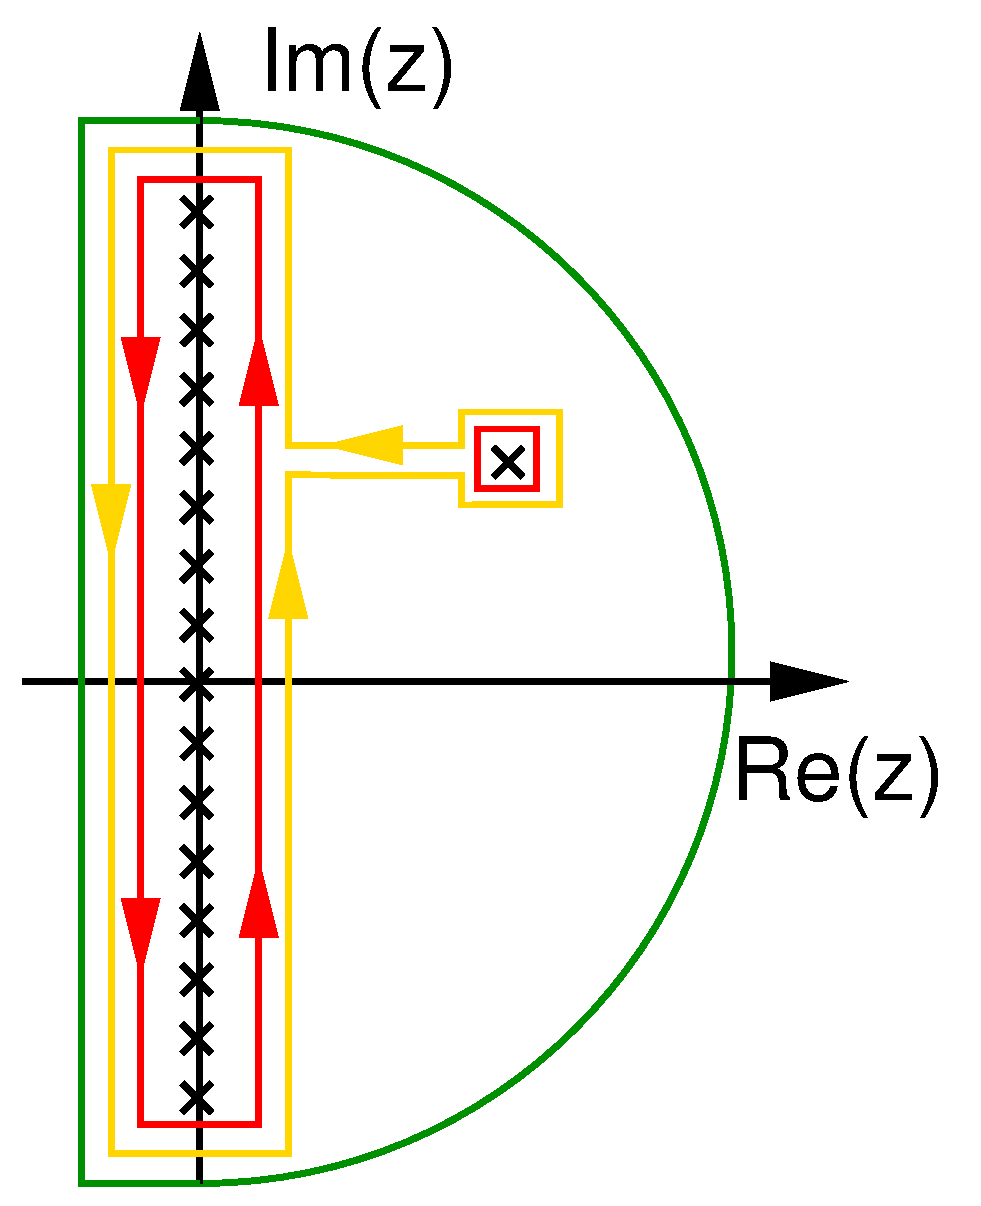
\includegraphics[width=0.25\linewidth]{Figs/Xfig/Matsubaracontour/contour.eps}
\end{center}

The integration is closed in the half plane with $\pm Re(z)>0$, because
we there the corresponding weighting function $h^{\pm}$ decays
exponentially for $Re(z)\rightarrow\pm\infty$.


%====================================================================
\subsection{Matsubara sums\index{Matsubara sum}}
%====================================================================
From \url{http://en.wikipedia.org/wiki/Matsubara_frequency} we obtain
the following expression for the \textbf{fermionic} summations.  In
these expressions the Matsubara frequencies are\footnote{They differ
  from those of the source by a factor $1/\hbar$.}
\begin{eqnarray}
\omega_\nu=(2\nu+1)\pi/(\hbar\beta)
\end{eqnarray}


\begin{eqnarray}
-k_BT\sum_\nu\ln[-i\hbar\omega_\nu+\epsilon]\e{i\omega_\nu0^+}
&=&-k_BT\ln[1+e^{-\beta \epsilon}]
\\
k_BT\sum_\nu \frac{1}{(i\hbar\omega_\nu-\epsilon)}\e{i\omega_\nu 0^+}
&=&(1+\e{\beta \epsilon})^{-1}
\\
k_BT\sum_\nu \frac{1}{(i\hbar\omega_\nu-\epsilon)^n}
&=&\frac{1}{(k_BT)^{n-1}(n-1)!}
\left.\partial_\epsilon^{n-1}\right|_{x=\beta\epsilon}(1+\e{x})^{-1}
\end{eqnarray}
\begin{center}
\begin{tabular}{|c|c|c|c|c|c|c|c|c|c|c|}
\hline
$j$& 1 & 2 & 3 & 4 & 5 &6 &7 &8 & 9 & 10\\
\hline
$\partial^{j-1}_x(1+\e{x})^{-1}$
&$\frac{1}{2}$ 
&$-\frac{1}{4}$ 
&$0$ 
&$+\frac{1}{8}$ 
&$0$ 
&$-\frac{1}{4}$ 
&$0$ 
&$\frac{17}{16}$
&$0$ 
&$-\frac{31}{4}$
\\
\hline
$\partial^{j-1}_x(1+\e{x})^{-1}$
&$0.5$ 
&$-0.25$ 
&$0$ 
&$+0.125$ 
&$0$ 
&$-0.25$ 
&$0$ 
&$+1.0625$
&$0$ 
&$-7.75$
\\
\hline
\hline
$j$& 11 & 12 & 13 & 14 & 15 &16 &17 &18 & 19 & 20\\
\hline
$\partial^{j-1}_x(1+\e{x})^{-1}$
&$0$ 
&$\frac{691}{8}$ 
&$0$ 
&$-\frac{5461}{4}$ 
&$0$ 
&$\frac{929569}{32}$ 
&$0$ 
&$-\frac{3202291}{4}$
&$0$ 
&$+\frac{221930581}{8}$
\\
\hline
$\partial^{j-1}_x(1+\e{x})^{-1}$
&$0$ 
&$86.375$ 
&$0$ 
&$-1365.25$ 
&$0$ 
&$29.0\times10^3$ 
&$0$ 
&$-800\times10^3$
&$0$ 
&$27.7\times 10^6$ %$+27741322.625$
\\
\hline
\end{tabular}
\end{center}

\begin{figure}[h!]
\begin{center}
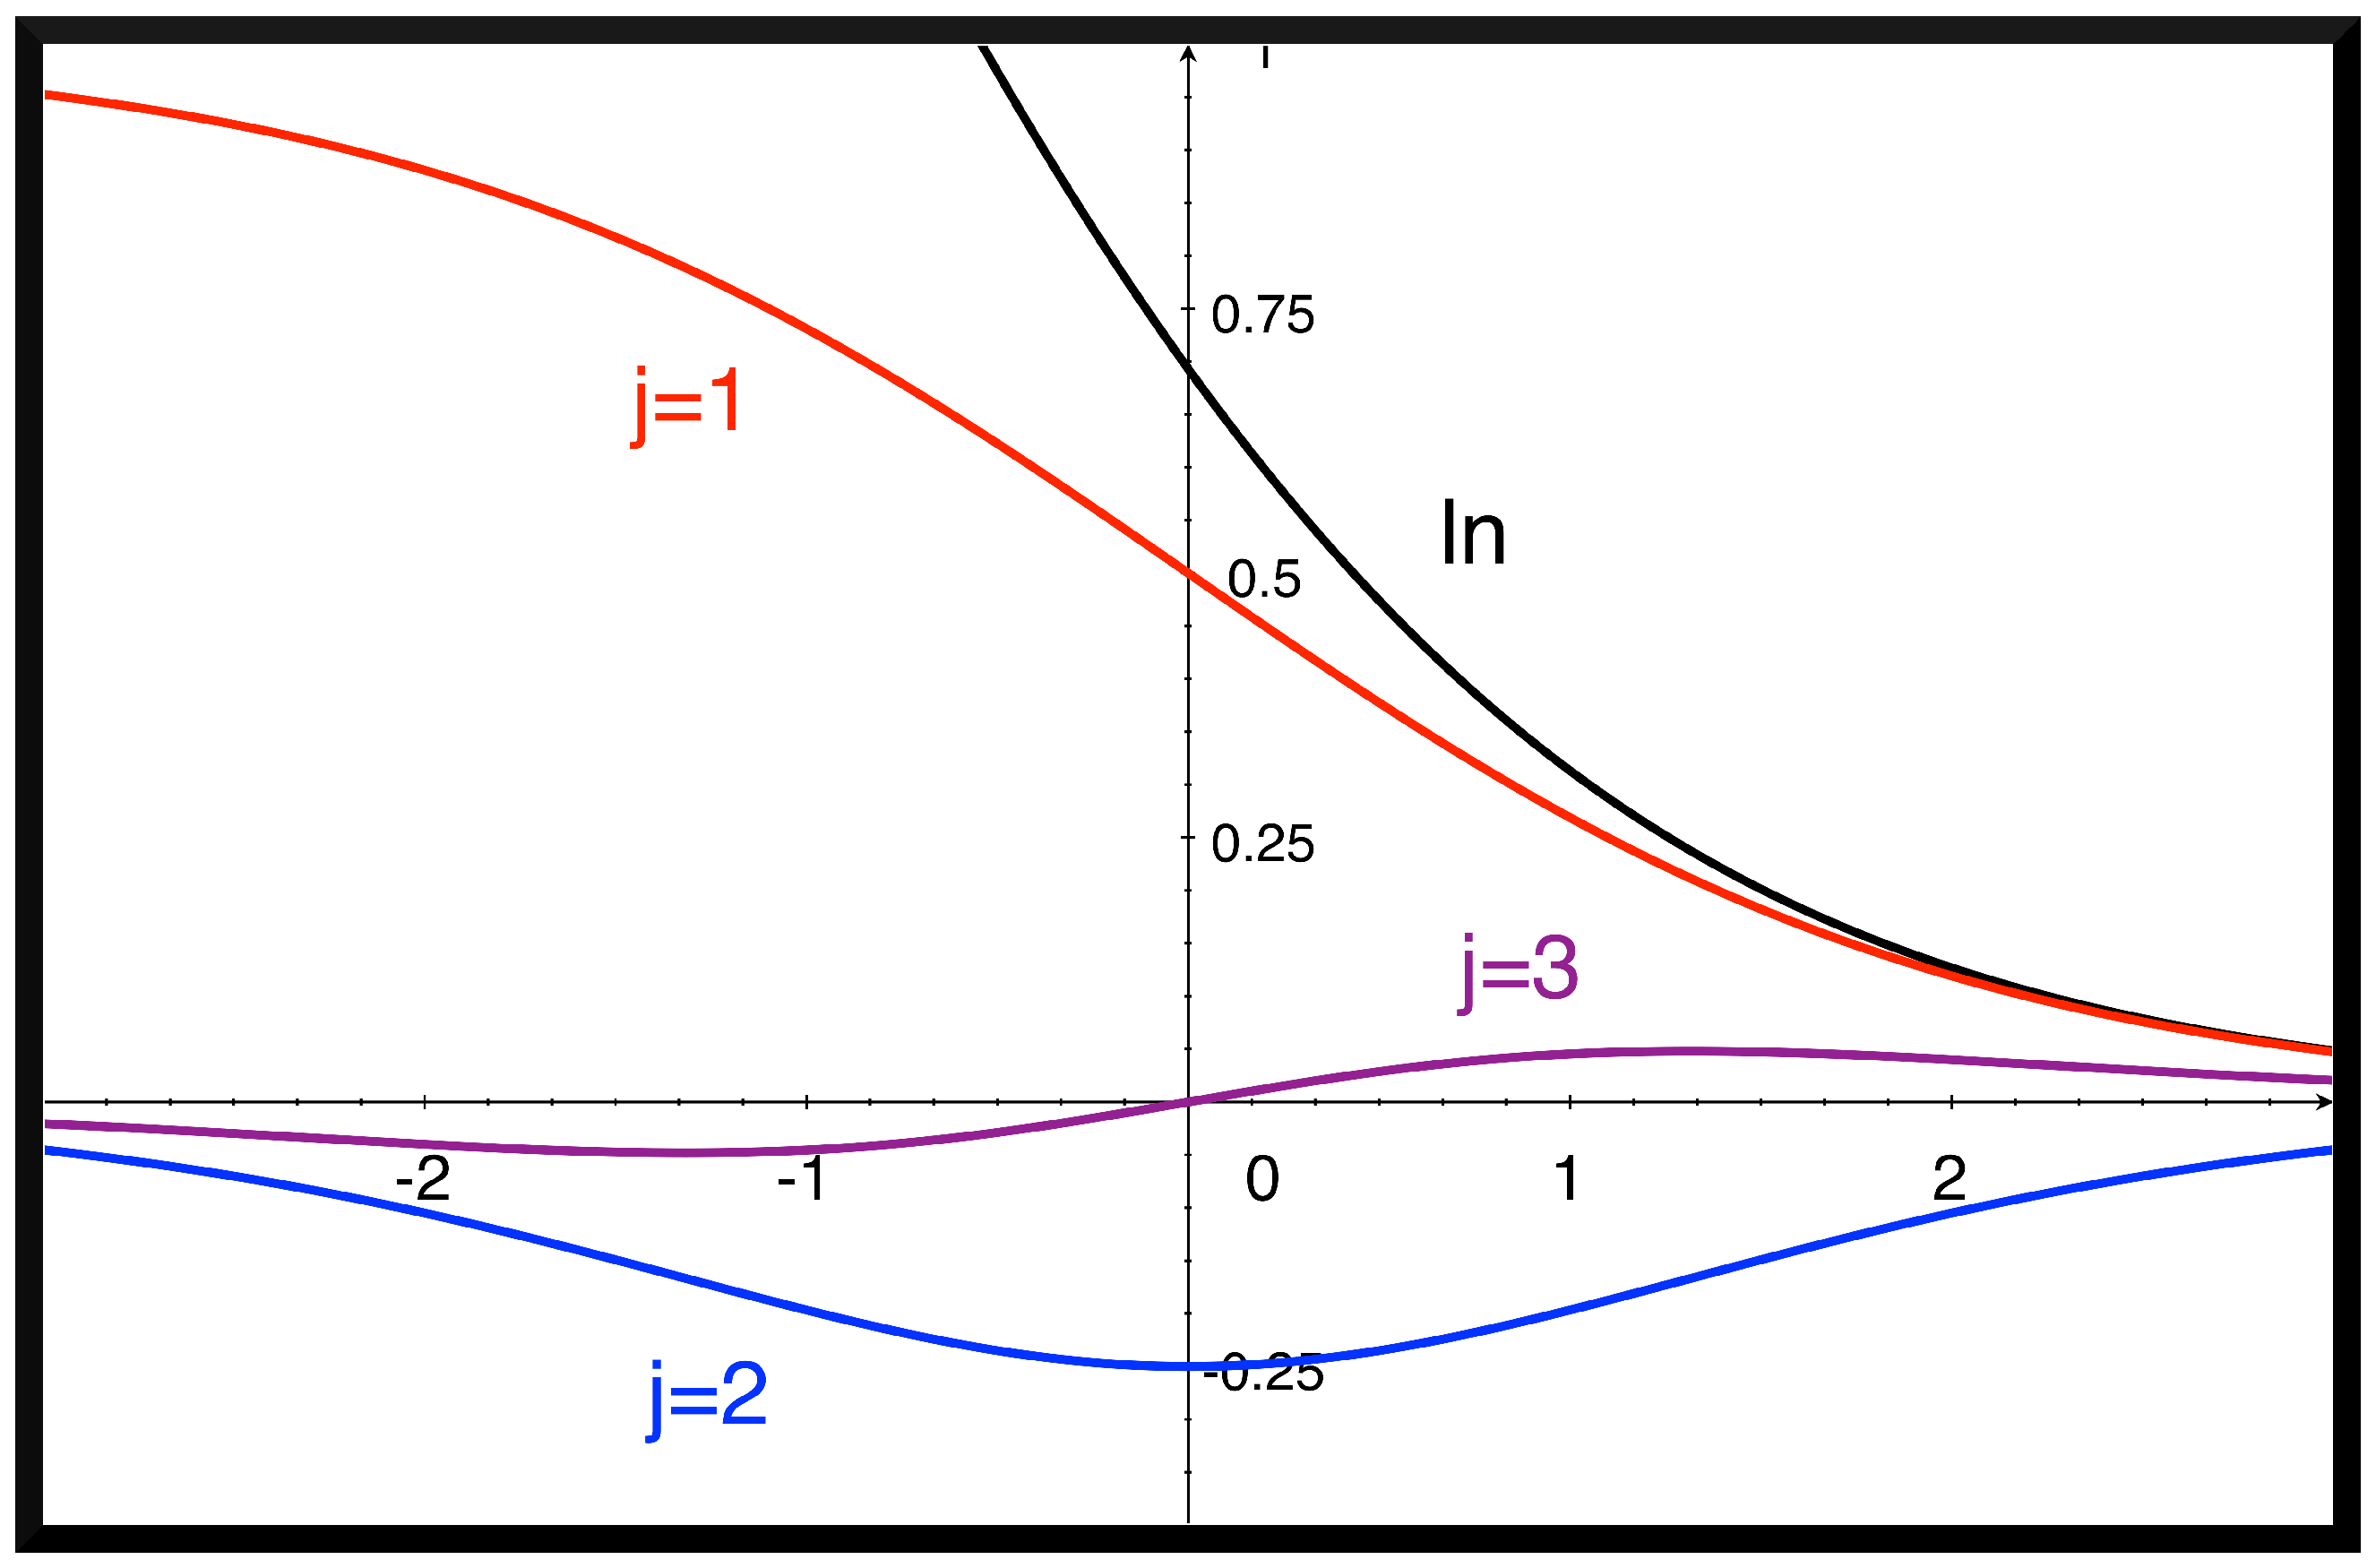
\includegraphics[width=0.8\linewidth,clip=true]
{Figs/Matsubarasums/matsubarasums1.eps}
\end{center}
\caption{\label{fig:matsubarasums} The result of Matsubara sums
  $-k_BT\sum_\nu\ln[-i\hbar\omega_\nu+\epsilon]$, $k_BT\sum_\nu
  \frac{1}{(i\hbar\omega_\nu-\epsilon)}\e{i\omega_\nu 0^+}$,
$k_BT\sum_\nu \frac{1}{(i\hbar\omega_\nu-\epsilon)^2}$ as
  function of energy $\epsilon$.}
\end{figure}



%====================================================================
\subsection{Matsubara sums on finite grids}
%====================================================================
The finite Matsubara sums result in a Fermi function that does not
reach zero or one. In particular, in the limit of e level, that lies
far from the chemical potential, the finite Matsubara sum falls off to
$\frac{1}{2}$.

\begin{figure}[h!]
\begin{center}
\includegraphics[width=0.4\linewidth,clip=true]
{Figs/Xmgrace/FiniteMatsubara/gsumlow.eps}
\includegraphics[width=0.4\linewidth,clip=true]
{Figs/Xmgrace/FiniteMatsubara/gsumhigh.eps}
\end{center}
\caption{\label{fig:finfitematsubara} Fermi function calculated from a
  finite Matsubara sum. The function is shifted by $-\frac{1}{2}$
  because no relgularization has been done. The sums have been
  performed with $2^n$ grid points with $n=0,\ldots,12$ for $k_BT=1.$}
\end{figure}



%====================================================================
\chapter{The Green function}
%====================================================================
%====================================================================
\section{Generic properties}
%====================================================================
%====================================================================
\subsection{Green's function with negative Matsubara frequencies}
%====================================================================
Green's functions and self energies obey the relation
\begin{eqnarray}
\mat{G}(-i\omega_\nu)=\mat{G}^\dagger(i\omega)
\label{eq:matsubaragnegfreq}
\end{eqnarray}
This allows one to store only half of the Green's functions.

Proof:

\begin{eqnarray}
G_{\alpha,\beta}(i\omega_n)&=&
-\frac{1}{\hbar}\int_0^{\hbar\beta} d\tau\;\e{i\omega_n\tau}
\Bigl\langle\mathcal{T}\hat{c}_\alpha(\tau)\hat{c}^\dagger_\beta(0)\Bigr\rangle
\\
\Rightarrow
G_{\alpha,\beta}(-i\omega_n)
&=&
-\frac{1}{\hbar}\int_0^{\hbar\beta} d\tau\;\e{-i\omega_n\tau}
\Bigl\langle\mathcal{T}\hat{c}_\alpha(\tau)\hat{c}^\dagger_\beta(0)\Bigr\rangle
\nonumber\\
&=&
\biggl\lbrace
-\frac{1}{\hbar}\int_0^{\hbar\beta} d\tau\;\e{i\omega_n\tau}
\Bigl\langle\biggl(\e{\beta(\hat{H}-\mu\hat{N})}\hat{c}_\alpha
\e{-\beta(\hat{H}-\mu\hat{N})}\hat{c}^\dagger_\beta\biggr)^\dagger
\Bigr\rangle
\biggr\rbrace^*
\nonumber\\
&=&
\biggl\lbrace
-\frac{1}{\hbar}\int_0^{\hbar\beta} d\tau\;\e{i\omega_n\tau}
\Bigl\langle
\hat{c}_\beta\e{-\beta(\hat{H}-\mu\hat{N})}\hat{c}^\dagger_\alpha
\e{\beta(\hat{H}-\mu\hat{N})}
\Bigr\rangle
\biggr\rbrace^*
\nonumber\\
&\stackrel{cycl. perm}{=}&
\biggl\lbrace
-\frac{1}{\hbar}\int_0^{\hbar\beta} d\tau\;\e{i\omega_n\tau}
\Bigl\langle
\e{\beta(\hat{H}-\mu\hat{N})}
\hat{c}_\beta\e{-\beta(\hat{H}-\mu\hat{N})}\hat{c}^\dagger_\alpha
\Bigr\rangle
\biggr\rbrace^*
\nonumber\\
&=&
\biggl\lbrace
-\frac{1}{\hbar}\int_0^{\hbar\beta} d\tau\;\e{i\omega_n\tau}
\Bigl\langle
\mathcal{T}\hat{c}_\beta(\tau)\hat{c}^\dagger_\alpha
\Bigr\rangle
\biggr\rbrace^*
\nonumber\\
&=&
G_{\beta,\alpha}^*(i\omega_\nu)
\end{eqnarray}

%====================================================================
\subsection{Density of states}
%====================================================================
For a system of independent electrons, the number of particles is
related to the chemical potential via
\begin{eqnarray}
N(\mu)=\int_{-\infty}^\infty d\epsilon\; f_\mu(\epsilon) D(\epsilon)
\;,
\end{eqnarray}
where $D$ is the density of states. $f_\mu(\epsilon)$ is the Fermi function.

\begin{eqnarray}
\frac{dN}{d\mu}
&=&\int_{-\infty}^\infty d\epsilon\; 
\frac{\partial f_\mu(\epsilon)}{\partial\mu} D(\epsilon)
=
\underbrace{\int_{-\infty}^\infty d\epsilon\; 
\frac{\beta}{\cosh^2\Bigl(\frac{1}{2}\beta(\epsilon-\mu)\Bigr)} D(\epsilon)
}_{\tilde{D}(\mu)}
\end{eqnarray}
Thus $dN/d\mu$ provides us with a broadened density of states.

Now we generalize the relation obtained for independent Fermions to
interacting Fermions. The number of states function $N_{a,b}(\mu)$ can
be obtained from the Green's function
\begin{eqnarray}
N_{a,b}(\mu)
&=&\frac{1}{\beta}\sum_\nu G_{a,b}(i\omega_\nu,\mu)\e{i\omega_\nu0^+}
=\frac{1}{\beta}\sum_\nu 
\biggl[
\Bigl(\mat{G}(i\omega_\nu,\mu_0)
\Bigr)^{-1}+(\mu-\mu_0)\biggr]^{-1}_{a,b}\e{i\omega_\nu0^+}
\end{eqnarray}

The smoothened density of states $\tilde{D}_{a,b}(\mu)$ is then
obtained as derivative with respect to $\mu$.
\begin{eqnarray}
\tilde{D}_{a,b}(\mu)&\defas&\frac{\partial N_{a,b}}{\partial\mu}
\nonumber\\
&=&
-\frac{1}{\beta}\sum_\nu 
\sum_c
\biggl[
\Bigl(\mat{G}(i\omega_\nu,\mu_0)
\Bigr)^{-1}+(\mu-\mu_0)\mat{1}\biggr]^{-1}_{a,c}
\biggl[
\Bigl(\mat{G}(i\omega_\nu,\mu_0)
\Bigr)^{-1}+(\mu-\mu_0)\mat{1}\biggr]^{-1}_{c,b}
\nonumber\\
\end{eqnarray}

This relation is however only valid for non-interacting electrons,
because a self energy may depend itself on the chemical potential.

%====================================================================
\section{Greens functions between band states and local orbitals}
%====================================================================
%====================================================================
\subsection{Lattice Greens functions and limited set of band states}
%====================================================================
We construct the \textbf{lattice Green's function} defined as
\begin{eqnarray}
\hat{G}^{lat}(i\omega_\nu)&=&
\biggl[(i\hbar\omega_\nu+\mu)\hat{1}
-\hat{h}-\Delta\hat{\Sigma}(i\omega_\nu)\biggr]^{-1}
\nonumber\\
&=&\sum_{n,n'}^\infty|\psi_n\rangle
\underbrace{
\biggl[\langle\psi_{n'}|(i\hbar\omega_\nu+\mu)\hat{1}-\hat{h}
-\Delta\hat{\Sigma}(i\omega_\nu)|\psi_n\rangle\biggr]_{n,n'}^{-1}
}_{G^{lat}_{n,n'}}
\langle\psi_{n'}|
\nonumber\\
&\approx&\sum_{n,n'}^{N_x}|\psi_n\rangle
\underbrace{
\biggl[\langle\psi_{n'}|(i\hbar\omega_\nu+\mu)\hat{1}-\hat{h}
-\Delta\hat{\Sigma}(i\omega_\nu)|\psi_n\rangle\biggr]_{n,n'}^{-1}
}_{G^{lat}_{n,n'}}
\langle\psi_{n'}|
\label{eq:latgreenfunc}
\end{eqnarray}
This expression is approximate, if the set of band states is not
complete. In practice, corrections are required.

In the representation of the band states, the lattice Green's function
has the form
\begin{eqnarray}
G^{lat}_{n,n'}(i\omega_\nu)&=&
\biggl[\langle\psi_{n'}|(i\hbar\omega_\nu+\mu)\hat{1}-\hat{h}
-\Delta\hat{\Sigma}(i\omega_\nu)|\psi_n\rangle\biggr]_{n,n'}^{-1}
\label{eq:latgreenfuncmat}
\end{eqnarray}
Note, that the matrix to be inverted is not necessarily hermitean!


%====================================================================
\subsection{Green's function on the Hilbert space of correlated orbitals}
%====================================================================
Here, we define the Green's function as inverse of a Hamiltonian,
which is projected onto a sub-Hilbert space of correlated
orbitals. 

We introduce the projection operator onto the correlated orbitals.
\begin{eqnarray}
\hat{\mathcal{P}}_\chi=\sum_{a,b}|\chi_a\rangle S^{-1}_{a,b}\langle\chi_b|
\qquad\text{with}\qquad \sum_c S^{-1}_{a,c}\langle\chi_c|\chi_b\rangle=\delta_{a,b}
\end{eqnarray}
onto the correlated orbitals. The projection operator is idempotent,
i.e. $\hat{\mathcal{P}}_\chi^2=\hat{\mathcal{P}}_\chi$

The Green's function is that operator that acts in the Hilbert space
of the correlated orbitals, and that inverts the Hamiltonian projected
onto that Hilbert space. Thus the following equation defines the
Greens function.
\begin{eqnarray}
\hat{G}\hat{\mathcal{P}}_\chi
\biggl[(i\hbar\omega_\nu+\mu)\hat{1}-\hat{h}-\sum_{c,d}|\pi_c\rangle\Sigma_{c,d}(i\omega_\nu)\langle\pi_d|\biggr]
\hat{\mathcal{P}}_\chi=\hat{\mathcal{P}}_\chi
\end{eqnarray}

We extract the matrix elements of the Green's function
$\hat{G}=|\chi\rangle\mat{G}\langle\chi|$.
\begin{eqnarray}
\underbrace{|\chi\rangle \mat{G}\langle\chi|}_{\hat{G}}
\underbrace{|\chi\rangle \mat{S}^{-1}\langle\chi|}_{\hat{\mathcal{P}}_\chi}
\biggl[(i\hbar\omega_\nu+\mu)\hat{1}-\hat{h}-\sum_{c,d}|\pi_c\rangle\Sigma_{c,d}(i\omega_\nu)\langle\pi_d|\biggr]
\underbrace{|\chi\rangle \mat{S}^{-1}\langle\chi|}_{\hat{\mathcal{P}}_\chi}
=\underbrace{|\chi\rangle \mat{S}^{-1}\langle\chi|}_{\hat{\mathcal{P}}_\chi}
\nonumber\\
\mat{G}\langle\chi|
\biggl[(i\hbar\omega_\nu+\mu)\hat{1}-\hat{h}-\sum_{c,d}|\pi_c\rangle\Sigma_{c,d}(i\omega_\nu)\langle\pi_d|\biggr]
|\chi\rangle =\mat{1}
\nonumber\\
\mat{G}
\biggl[(i\hbar\omega_\nu+\mu)\mat{S}-\langle\chi|\hat{h}|\chi\rangle-\mat{\Sigma}(i\omega_\nu)\biggr]
=\mat{1}
\nonumber\\
\end{eqnarray}
which yields with $\hat{h}=\sum_n|\psi_n\rangle\epsilon_n\langle\chi_n|$
\begin{eqnarray}
\mat{G}&=&
\biggl[(i\hbar\omega_\nu+\mu)\mat{S}
-\sum_{n=1}^\infty
\langle\chi|\psi_n\rangle \epsilon_n\langle\psi_n|\chi\rangle-\mat{\Sigma}(i\omega_\nu)\biggr]^{-1}
\end{eqnarray}

This expression involves still an infinite sum over band states, which
are not all available in practice. In order to remedy this deficiency
without introducing major errors, we modify the spectrum of of the
Hamiltonian in an energy region above the partially occupied states.
This approximation can be controlled by increasing the number $N_x$ of
states that are explicitely included in the sum. Specifically, we
change all eigenvalues with a band index higher than $N_x$ of the
Hamiltonian to $\epsilon_x$.

This transforms the Hamiltonian into its approximate form
\begin{eqnarray}
\hat{h}\rightarrow\sum_{n=1}^{N_x}|\psi_n\rangle \epsilon_n\langle\psi_n|
+\sum_{n=N_x+1}^\infty|\psi_n\rangle \epsilon_x\langle\psi_n|
\end{eqnarray}
The approximation allows one to limit the sum over states to a finite sum.
\begin{eqnarray}
\mat{G}&=&
\biggl[(i\hbar\omega_\nu+\mu-\epsilon_x)\mat{S}-\sum_{n=1}^{N_x}
\langle\chi|\psi_n\rangle (\epsilon_n-\epsilon_x)\langle\psi_n|\chi\rangle-\mat{\Sigma}(i\omega_\nu)\biggr]^{-1}
\end{eqnarray}


After limiting the sum over the states that can be well represented by
the correlated orbitals, we use the approximation
$|\psi_n\rangle=\sum_a|\chi_a\rangle\langle\pi_a|\psi_n\rangle$, which
yields
\begin{eqnarray}
\langle\chi|\psi\rangle
=\langle\chi|\chi\rangle\langle\pi|\hat{\mathcal{P}}_\chi|\psi\rangle
=\mat{S}\langle\pi|\hat{\mathcal{P}}_\chi|\psi\rangle
\approx 
\mat{S}\langle\pi|\psi\rangle
\end{eqnarray}
The results depends on how well the band states are representable by
the correlated orbitals. Thus, it is important to limit the sum over
band states to those that are well represented by tight-binding
orbitals. Furthermore one should always include a as complete as
possible set of correlated orbiatals, rather that just limiting
oneself to particular atoms. A potential test of this approximation is
to evaluate the effect on the orthonormality of the band states in the
form 
\begin{eqnarray}
\delta_{n,m}=\langle\psi_n|\psi_m\rangle
\approx\sum_{a,b}
\langle\psi_n|\pi_a\rangle\langle\chi_a|\chi_b\rangle\langle\pi_b|\psi_m\rangle
=\sum_{a,b}
\langle\psi_n|\pi_a\rangle S_{a,b} \langle\pi_b|\psi_m\rangle
\end{eqnarray}
  
With this approximation we obtain
\begin{myshadowminipage}{Greens function projected}
\begin{eqnarray}
\mat{G}&=&
\biggl[(i\hbar\omega_\nu+\mu-\epsilon_x)\mat{S}-\sum_{n=1}^{N_x}
\mat{S}\langle\pi|\psi_n\rangle (\epsilon_n-\epsilon_x)\langle\psi_n|\pi\rangle\mat{S}-\mat{\Sigma}(i\omega_\nu)\biggr]^{-1}
\end{eqnarray}
\end{myshadowminipage}

This matrix corresponds to
\begin{eqnarray}
\mat{G}&=&
\biggl[(i\hbar\omega_\nu+\mu)\mat{S}-\mat{\bar{h}}+\mat{\Gamma}
-\mat{\Sigma}(i\omega_\nu)\biggr]^{-1}
\end{eqnarray}
which allows one to make the identification (for full selfconsistency)
\begin{eqnarray}
\epsilon_x
\biggl[\mat{S}
-\sum_{n=1}^{N_x}
\mat{S}\langle\pi|\psi_n\rangle\langle\psi_n|\pi\rangle\mat{S}\biggr]
-
\underbrace{\sum_{n=1}^{N_x}
\mat{S}\langle\pi|\psi_n\rangle\epsilon_n\langle\psi_n|\pi\rangle\mat{S}
}_{\rightarrow \frac{\hat{\vec{p}}^2}{2m}+v_{ext}+v_H+v_{xc}}
=-\mat{\bar{h}}+\mat{\Gamma}
\nonumber\\
\Rightarrow\qquad
\mat{\bar{h}}
=
\underbrace{\sum_{n=1}^{N_x}
\mat{S}\langle\pi|\psi_n\rangle\epsilon_n\langle\psi_n|\pi\rangle\mat{S}
}_{\rightarrow \frac{\hat{\vec{p}}^2}{2m}+v_{ext}+v_H+v_{xc}}
-\epsilon_x
\biggl[\mat{S}
-\sum_{n=1}^{N_x}
\mat{S}\langle\pi|\psi_n\rangle\langle\psi_n|\pi\rangle\mat{S}\biggr]
+\mat{\Gamma}
\end{eqnarray}


%====================================================================
\section{Project Green's function onto local orbitals}
%====================================================================
For a Hamiltonian $\hat{h}=\sum_{a,b}|\pi_a\rangle
h_{a,b}\langle\pi_b|$ and a self energy 
$\hat{\Sigma}(i\omega_\nu)=
\sum_{a,b}|\pi_a\rangle
\Sigma_{a,b}(i\omega_\nu)
\langle\pi_b|$
acting on the local orbitals, the Green's function can be expressed
as
\begin{eqnarray}
\hat{G}(i\omega_\nu)&=&
\sum_{a,b}|\chi_a\rangle
\biggl\lbrace
\sum_{n,n'}\langle\pi_a|\psi_n\rangle
\biggl[
(i\hbar\omega_\nu+\mu)\delta_{n,n'}
\nonumber\\
&&-\sum_{c,d}\langle\psi_n|\pi_c\rangle
\Bigl(h_{c,d}+\Sigma_{c,d}(i\omega_\nu)\Bigr)
\langle\pi_d|\psi_{n'}\rangle
\biggr]^{-1}_{n,n'}
\langle\psi_{n'}|\pi_b\rangle
\biggr\rbrace
\langle\chi_b|
\label{eq:greenlocorb}
\end{eqnarray}
We converted Eq.~\eqref{eq:latgreenfunc} into a basis of local
orbitals $|\chi_a\rangle$ using
$|\psi_n\rangle=\sum_a|\chi_a\rangle\langle\pi_a|\psi_n\rangle$.


In order to evaluate the Green's function, we still need to refer to the
band states. The Green's function can, however, also be expressed
without making direct use of the band states, namely as
\begin{myshadowminipage}{Green's function in matrix form}
For a hamiltonian $\hat{h}$ and a self energy $\hat{\Sigma}$ that can
be expressed entirely in terms of projector functions, the Green's
function in the approximate form of \eq{eq:latgreenfunc} has the form
\begin{eqnarray}
\hat{G}(i\omega_\nu)=\sum_{a,b}|\chi_a\rangle
G_{a,b}(i\omega_\nu)\langle\chi_b|
\end{eqnarray}
with
\begin{eqnarray}
&&G_{a,b}(i\omega_\nu)
\nonumber\\
&=&
\biggl\lbrace
\sum_{n,n'}\langle\pi_a|\psi_n\rangle
\biggl[
(i\hbar\omega_\nu+\mu)\delta_{n,n'}
-\sum_{c,d}\langle\psi_n|\pi_c\rangle
\Bigl(h_{c,d}+\Sigma_{c,d}(i\omega_\nu)\Bigr)
\langle\pi_d|\psi_{n'}\rangle
\biggr]^{-1}_{n,n'}
\langle\psi_{n'}|\pi_b\rangle
\biggr\rbrace
\nonumber\\
&=&\biggl[(i\hbar\omega_\nu+\mu)\mat{S}
-\mat{h}-\mat{\Sigma}(i\omega_\nu)\biggr]^{-1}
\label{eq:greenlocform1}
\end{eqnarray}
where\footnote{in a representation of Bloch states the inverse overlap
  calculation is calculated for each k-point and inverted.}
\begin{eqnarray}
S^{-1}_{a,b}=\langle\pi_a|\psi_n\rangle \langle\psi_n|\pi_b\rangle
\label{eq:inverses}
\end{eqnarray}
\end{myshadowminipage}





\textbf{Proof:}
Here, I will show that the Green's function matrix 
\begin{eqnarray}
\mat{G}_{a,b}(i\omega_\nu)=
\sum_n\langle\pi_a|\psi_n\rangle
\biggl[
(i\hbar\omega_\nu+\mu)\delta_{n,n'}-
\sum_{c,d}\langle\psi_n|\pi_c\rangle
\Bigl(\mat{h}_{c,d}+\mat{\Sigma}_{c,d}(i\omega_\nu)\Bigr)
\langle\pi_d|\psi_{n'}\rangle
\biggr]^{-1}_{n,n'}
\langle\psi_{n'}|\pi_b\rangle
\nonumber\\
\label{eq:greenlocform2}
\end{eqnarray}
can be expressed in the form of \eq{eq:greenlocform1}.

In order to simplify the proof, I will not write out the self energy,
nor the chemical potential. This is possible because the proof works
for each Matsubara frequency independently, so that both can be
absorbed in the non-interacting Hamiltonian.
\begin{eqnarray}
G_{a,b}(i\omega_\nu)
&=&
\sum_{n,n'}\langle\pi_a|\psi_{n}\rangle
\biggl(i\hbar\omega_\nu\delta_{n,n'}
-
\langle\psi_n|\pi\rangle
\mat{h}
\langle\pi|\psi_{n'}\rangle\biggr)^{-1}_{n,n'}
\langle\psi_{n'}|\pi_b\rangle
\nonumber\\
&=&
\sum_{n,n'}\langle\pi_a|\psi_{n}\rangle
\biggl[
\sum_{j=0}^\infty
\frac{1}{(i\hbar\omega_\nu)^{j+1}}
\biggl(
\langle\psi|\pi\rangle
\mat{h}
\langle\pi|\psi\rangle\biggr)^j_{n,n'}
\biggr]\langle\psi_{n'}|\pi_b\rangle
\nonumber\\
&=&
\sum_{n,n'}\langle\pi_a|\psi_{n}\rangle
\biggl[
\sum_{j=0}^\infty
\frac{1}{(i\hbar\omega_\nu)^{j+1}}
\biggl(\sum_{n_2,\ldots,n_{j}} 
\langle\psi_{n}|\pi\rangle
\mat{h}
\langle\pi|\psi_{n_2}\rangle\langle\psi_{n_2}|\pi\rangle
\ldots
\mat{h}
\langle\pi|\psi_{n'}\rangle\biggr)\biggr]
\langle\psi_{n'}|\pi_b\rangle
\nonumber\\
&=&
\sum_{j=0}^\infty\frac{1}{(i\hbar\omega_\nu)^{j+1}}
\biggl(\sum_{n_1,\ldots,n_{j+1}} 
\underbrace{\langle\pi|\psi_{n_1}\rangle
\langle\psi_{n_1}|\pi\rangle}_{\mat{S}^{-1}}
\mat{h}
\underbrace{\langle\pi|\psi_{n_2}\rangle\langle\psi_{n_2}|\pi\rangle}_{\mat{S}^{-1}}
\ldots
\mat{h}
\underbrace{\langle\pi|\psi_{n_{j+1}}\rangle
\langle\psi_{n_{j+1}}|\pi\rangle}_{\mat{S}^{-1}}
\biggr)_{a,b}
\nonumber\\
&=&
\biggl(\sum_{j=0}^\infty\frac{1}{(i\hbar\omega_\nu)^{j+1}}
\biggl(\mat{S}^{-1}\mat{h}\biggr)^{j}\mat{S}^{-1}\biggr)_{a,b}
\nonumber\\
&=&\biggl[i\hbar\omega_\nu\mat{S}\biggl
(\mat{1}-\frac{1}{i\hbar\omega_\nu}\mat{S}^{-1}\mat{h}\Bigr)\biggr]^{-1}_{a,b}
\nonumber\\
&=&\biggl[i\hbar\omega_\nu\mat{S}-\mat{h}\biggr]^{-1}_{a,b}
\end{eqnarray}
q.e.d.


%============================================================
\subsection{Laurent expansion of the non-interacting Green's function}
%============================================================
We determine the Laurent expansion terms of $\bar{\mat{G}}$
\begin{eqnarray}
\bar{\mat{G}}=\Bigl[i\hbar\omega_\nu\mat{S}-\Bigl(\bar{\mat{h}}-\mu\mat{S}\Bigr)
\Bigr]^{-1}
=\sum_{j=1}^\infty\frac{1}{(i\hbar\omega_\nu)^j}
\bar{\mathcal{\mat{G}}}^{(j)}
\end{eqnarray}
and therefore
\begin{eqnarray}
\mat{1}
&=&
\sum_{j=1}\frac{1}{(i\hbar\omega_\nu)^j}\bar{\mathcal{\mat{G}}}^{(j)}
\Bigl[i\hbar\omega_\nu\mat{S}-\Bigl(\bar{\mat{h}}-\mu\mat{S}\Bigr)
\Bigr]
\nonumber\\
&=&
\sum_{j=0}\frac{1}{(i\hbar\omega_\nu)^{j}}\bar{\mathcal{\mat{G}}}^{(j+1)}\mat{S}
-\sum_{j=1}\frac{1}{(i\hbar\omega_\nu)^j}\bar{\mathcal{\mat{G}}}^{(j)}\Bigl(\bar{\mat{h}}-\mu\mat{S}\Bigr)
\nonumber\\
\bar{\mathcal{\mat{G}}}^{(1)}
&=&\mat{S}^{-1}
\nonumber\\
\bar{\mathcal{\mat{G}}}^{(j+1)}
&=&\bar{\mathcal{\mat{G}}}^{(j)}\Bigl(\bar{\mat{h}}-\mu\mat{S}\Bigr)\mat{S}^{-1}
\qquad\text{for $j>1$}
\nonumber\\
\bar{\mathcal{\mat{G}}}^{j}&=&
\mat{S}^{-1}\biggl[\Bigl(\bar{\mat{h}}-\mu\mat{S}\Bigr)\mat{S}^{-1}\biggr]^{j-1}
\label{eq:laurentexpansionofgbar}
\end{eqnarray}

The first term in the Laurent expansion of $\mat{G}-\bar{\mat{G}}$ vanishes
\begin{eqnarray}
\mathcal{\mat{G}}^{(1)}-\bar{\mathcal{\mat{G}}}^{(1)}&=&0
\end{eqnarray}

%====================================================================
\subsection{Laurent expansion of the Green's function (new)}
\label{sec:laurentgreen}
%====================================================================
In order to regularize the Matsubara sums, respectively, to limit the
extent of the Matsubara sum evaluated numerically, we need to
represent the Green's function for high frequencies in terms of
Matsubara sums.

Here, we extract the Laurent expansion of the Green's function in the form
\begin{eqnarray}
\mat{G}=\biggl[(i\hbar\omega_\nu+\mu)\mat{S}
-\mat{h}-\mat{\Sigma}(i\omega_\nu)\biggr]^{-1}
\end{eqnarray}
where the self energy has the Laurent expansion
\begin{eqnarray}
\mat{\Sigma}(i\omega_\nu)
=\sum_{j=0}^\infty\frac{1}{(i\hbar\omega_\nu)^j}\mathcal{S}^{(j)}
\end{eqnarray}

Thus the numerical representation of the Green's function is
\begin{eqnarray}
\mat{G}(i\omega_\nu)=
\begin{cases}
\biggl[(i\hbar\omega_\nu+\mu)\mat{S}
-\mat{h}-\mat{\Sigma}(i\omega_\nu)\biggr]^{-1}
&\text{for $|\nu|\le\nu_x$}\\
\biggl[(i\hbar\omega_\nu+\mu)\mat{S}
-\mat{h}-\sum_{j'=0}^{j_x'}\mat{\mathcal{S}}^{(j')}\frac{1}{(i\hbar\omega_\nu)^{j'}}
\biggr]^{-1}
&\text{for $|\nu|>\nu_x$}
\end{cases}
\end{eqnarray}


The high-frequency representation of the Green's function shall itself
be represented by a Laurent expansion
\begin{eqnarray}
\mat{G}(i\omega_\nu)=\sum_{j=1}^\infty\mat{\mathcal{G}}^{(j)}
\frac{1}{(i\hbar\omega_\nu)^j}
\end{eqnarray}

The identity 
\begin{eqnarray}
\sum_{j=1}^\infty\mat{\mathcal{G}}^{(j)}
\frac{1}{(i\hbar\omega_\nu)^j}
&=&
\biggl[(i\hbar\omega_\nu+\mu)\mat{S}
-\mat{h}
-\sum_{j'=0}^{j_x'}\mat{\mathcal{S}}^{(j')}\frac{1}{(i\hbar\omega_\nu)^{j'}}
\biggr]^{-1}
\end{eqnarray}
yields
\begin{eqnarray}
\sum_{j=1}^\infty\mat{\mathcal{G}}^{(j)}
\frac{1}{(i\hbar\omega_\nu)^j}
\biggl[(i\hbar\omega_\nu+\mu)\mat{S}
-\mat{h}-\sum_{j'=0}^{j_x'}\mat{\mathcal{S}}^{(j')}\frac{1}{(i\hbar\omega_\nu)^{j'}}
\biggr]=\mat{1}
\end{eqnarray}
which we can be arranged in orders of inverse Matsubara frequencies
\begin{eqnarray}
\sum_{j=0}^\infty\mat{\mathcal{G}}^{(j+1)}\mat{S}\frac{1}{(i\hbar\omega_\nu)^j}
+
\sum_{j=1}^\infty\mat{\mathcal{G}}^{(j)}
\biggl[\mu\mat{S}-\mat{h}-\mat{\mathcal{S}}^{(0)}\Bigr]
\frac{1}{(i\hbar\omega_\nu)^j}
\nonumber\\
-\sum_{j=2}^\infty
\sum_{n=1}^{j_x'}\mat{\mathcal{G}}^{(j-n)}\mat{\mathcal{S}}^{(n)}
\frac{1}{(i\hbar\omega_\nu)^j}
=\mat{1}
\end{eqnarray}

Thus, the expansion coefficients are
\begin{eqnarray}
\mat{\mathcal{G}}^{(1)}&=&\mat{S}^{-1}
\nonumber\\
\mat{\mathcal{G}}^{(j+1)}
&=&-
\mat{\mathcal{G}}^{(j)}
\biggl[\mu\mat{S}-\mat{h}-\mat{\mathcal{S}}^{(0)}\Bigr]\mat{S}^{-1}
+\sum_{n=1}^{min(j_x',j-1)}\mat{\mathcal{G}}^{(j-n)}\mat{\mathcal{S}}^{(n)}\mat{S}^{-1}
\qquad\text{for $j>0$}
\end{eqnarray}


Let us make the higher-order terms more explicit
\begin{eqnarray}
\mat{\mathcal{G}}^{(1)}&=&\mat{S}^{-1}
\nonumber\\
\mat{\mathcal{G}}^{(2)}
&=&-
\mat{\mathcal{G}}^{(1)}
\biggl[\mu\mat{S}-\mat{h}-\mat{\mathcal{S}}^{(0)}\Bigr]\mat{S}^{-1}
=-
\mat{S}^{-1}\biggl[\mu\mat{S}-\mat{h}-\mat{\mathcal{S}}^{(0)}\Bigr]\mat{S}^{-1}
\nonumber\\
\mat{\mathcal{G}}^{(3)}
&=&-
\mat{\mathcal{G}}^{(2)}
\biggl[\mu\mat{S}-\mat{h}-\mat{\mathcal{S}}^{(0)}\Bigr]\mat{S}^{-1}
+\mat{\mathcal{G}}^{(1)}\mat{\mathcal{S}}^{(1)}\mat{S}^{-1}
\nonumber\\
&=&
\mat{S}^{-1}\biggl[\mu\mat{S}-\mat{h}-\mat{\mathcal{S}}^{(0)}\Bigr]\mat{S}^{-1}
\biggl[\mu\mat{S}-\mat{h}-\mat{\mathcal{S}}^{(0)}\Bigr]\mat{S}^{-1}
+
\mat{S}^{-1}\mat{\mathcal{S}}^{(1)}\mat{S}^{-1}
\label{eq:Lauenttermsgreenappendix}
\end{eqnarray}
In practice, we expand the Green's function up to $\mathcal{G}^{(3)}$
and the self energy up to $\mathcal{S}^{(1)}$.


Thus the Green's function will be represented in the form
\begin{eqnarray}
\mat{G}(i\omega_\nu)=
\begin{cases}
\biggl[(i\hbar\omega_\nu+\mu)\mat{S}
-\mat{h}-\mat{\Sigma}(i\omega_\nu)\biggr]^{-1}
&\text{for $|\nu|\le\nu_x$}\\
\sum_{j=1}^3\mat{\mathcal{G}}^{(j)}\frac{1}{(i\hbar\omega_\nu)^j}
&\text{for $|\nu|>\nu_x$}
\end{cases}
\end{eqnarray}
where the Laurent-expansion coefficients of the Green's function are
defined in eq{eq:Lauenttermsgreenappendix}. The variational degrees of
freedom for the Greens functrion is the Green's function for
$0<\omega_\nu\le\omega_x$ and the first two Laurent-expansion terms
$\mat{\mathcal{S}}^{(0)}$ and $\mat{\mathcal{S}}^{(1)}$ of the self
energy. The Green's functiuon for negative Matsubara frequencies are
obtained by \eq{eq:matsubaragnegfreq},
$\mat{G}(-\i\omega_\nu)=\mat{G}^\dagger(\i\omega_\nu)$.

%============================================================
\subsubsection{Laurent-expansion coefficients are Hermitean}
%============================================================
The expansion coefficients for the Laurent expansion are hermitian.
We exploit that $\mat{G}(-i\omega_\nu)=\mat{G}^\dagger(i\omega_\nu)$
\begin{eqnarray}
\sum_{j=1}^\infty\frac{1}{(-i\hbar\omega_\nu)^j}\mat{\mathcal{G}}^{(j)}
=\mat{G}(-i\omega_\nu)&=&\mat{G}^\dagger(i\omega_\nu)
=\sum_{j=1}^\infty\frac{1}{(-i\hbar\omega_\nu)^j}
\left(\mat{\mathcal{G}}^{(j)}\right)^\dagger
\nonumber\\
\Rightarrow\qquad
\mat{\mathcal{G}}^{(j)}&=&\left(\mat{\mathcal{G}}^{(j)}\right)^\dagger
\end{eqnarray}

From this requirement we can derive that $\mat{S}$, $\mat{h}$,
$\mat{\mathcal{S}}^{(0)}$ and $\mat{\mathcal{S}}^{(0)}$ are hermitian as well.

%============================================================
\subsubsection{Difference of Green's functions}
%============================================================
The difference of two Green's function with different self energies
has the form
\begin{eqnarray}
\Delta\mat{\mathcal{G}}^{(1)}&=&0
\\
\Delta\mat{\mathcal{G}}^{(2)}&=&
\mat{S}^{-1}\mat{\mathcal{S}}^{(0)}\mat{S}^{-1}
\\
\Delta\mat{\mathcal{G}}^{(3)}
&=&
-\mat{S}^{-1}\biggl[\mu\mat{S}-\mat{h}\Bigr]\mat{S}^{-1}
\mat{\mathcal{S}}^{(0)}\mat{S}^{-1}
-\mat{S}^{-1}\mat{\mathcal{S}}^{(0)}\mat{S}^{-1}
\biggl[\mu\mat{S}-\mat{h}\Bigr]\mat{S}^{-1}
\nonumber\\
&&+\mat{S}^{-1}\mat{\mathcal{S}}^{(0)}\mat{S}^{-1}\mat{\mathcal{S}}^{(0)}
\mat{S}^{-1}
+
\mat{S}^{-1}\mat{\mathcal{S}}^{(1)}\mat{S}^{-1}
\end{eqnarray}

%==============================================================================
\subsubsection{Laurent expansion for the density matrix}
%==============================================================================
With this expression, we obtain the Matsubara sum required for the
density matrix as
\begin{eqnarray*}
\frac{1}{\beta}\sum_\nu\mat{G}\e{i\omega_\nu0^+}
&=&\sum_{j=1}^\infty
\left.\mat{\mathcal{G}}^{(j)}\frac{1}{(j-1)!}
\partial^{j-1}_\epsilon\right|_{\epsilon=0}(1+\e{\beta\epsilon})^{-1}
\nonumber\\
&=&
\frac{1}{2}\mat{\mathcal{G}}^{(1)}
-\frac{1}{4}\beta\mat{\mathcal{G}}^{(2)}
-0\cdot\beta^2\mat{\mathcal{G}}^{(3)}
+\underbrace{\Bigl(
\frac{1}{3!}\frac{1}{8}\beta^3\mat{\mathcal{G}}^{(4)}
-\frac{1}{5!}\frac{1}{4}\beta^5\mat{\mathcal{G}}^{(6)}
+\frac{1}{7!}1.0?\beta^7\mat{\mathcal{G}}^{(8)}\Bigr)
}_{\text{from grapher}}
+O(\beta^9)
\nonumber\\
&=&
\frac{1}{2}\mat{\mathcal{G}}^{(1)}
-\frac{1}{4}\beta\mat{\mathcal{G}}^{(2)}
+\underbrace{\Bigl(
\frac{1}{48}\beta^3\mat{\mathcal{G}}^{(4)}
-\frac{1}{480}\beta^5\mat{\mathcal{G}}^{(6)}
+\frac{1.0?}{4320}\beta^7\mat{\mathcal{G}}^{(8)}\Bigr)}_{\text{from grapher}}
+O(\beta^9)
\end{eqnarray*}


%==============================================================================
\subsubsection{Derivative of the Luttinger Ward functional}
%==============================================================================
For $j'\in\{0,1\}$
\begin{eqnarray}
\frac{\partial\Phi^{LW}_\beta}{\partial \mat{\mathcal{S}}^{(j')}}
&=&
\sum_{j=1}^3
\frac{1}{\beta}\sum_{\nu; |\nu|>\nu_x}
\frac{\beta\partial\Phi^{LW}_\beta}{\partial \mat{G}(i\omega_\nu)}
\frac{\partial \mat{G}(i\omega_\nu)}{\partial \mat{\mathcal{G}}^{(j)}}
\frac{\partial \mat{\mathcal{G}}^{(j)}}{\partial \mat{\mathcal{S}}^{(j')}}
\nonumber\\
&=&
\sum_{j=1}^3
\Bigl[\frac{1}{\beta}\sum_{\nu; |\nu|>\nu_x}
\frac{\beta\partial\Phi^{LW}_\beta}{\partial \mat{G}(i\omega_\nu)}
\frac{1}{(i\hbar\omega_\nu)^j}\Bigr]
\frac{\partial \mat{\mathcal{G}}^{(j)}}{\partial \mat{\mathcal{S}}^{(j')}}
\nonumber\\
\frac{\partial\Phi^{LW}_\beta}{\partial \mat{\mathcal{S}}^{(0)}}
&=&
\mat{S}^{-1}
\underbrace{\Bigl[\frac{1}{\beta}\sum_{\nu; |\nu|>\nu_x}
\frac{\beta\partial\Phi^{LW}_\beta}{\partial \mat{G}(i\omega_\nu)}
\frac{1}{(i\hbar\omega_\nu)^2}\Bigr]}
_{\delta\Phi^{LW}_{\beta,dyn}/\delta\mathcal{\mat{G}}^{(2)}}
\mat{S}^{-1}
\nonumber\\
&-&
\mat{S}^{-1}
\underbrace{\biggl[\frac{1}{\beta}\sum_{\nu; |\nu|>\nu_x}
\frac{\beta\partial\Phi^{LW}_\beta}{\partial \mat{G}(i\omega_\nu)}
\frac{1}{(i\hbar\omega_\nu)^3}\biggr]}
_{\delta\Phi^{LW}_{\beta,dyn}/\delta\mathcal{\mat{G}}^{(3)}}
\mat{S}^{-1}\Bigl[\mu\mat{S}-\mat{h}-\mat{\mathcal{S}}^{(0)}\Bigr]\mat{S}^{-1}
\nonumber\\
&-&
\mat{S}^{-1}
\Bigl[\mu\mat{S}-\mat{h}-\mat{\mathcal{S}}^{(0)}\Bigr]\mat{S}^{-1}
\underbrace{\biggl[\frac{1}{\beta}\sum_{\nu; |\nu|>\nu_x}
\frac{\beta\partial\Phi^{LW}_\beta}{\partial \mat{G}(i\omega_\nu)}
\frac{1}{(i\hbar\omega_\nu)^3}\biggr]}
_{\delta\Phi^{LW}_{\beta,dyn}/\delta\mathcal{\mat{G}}^{(3)}}
\mat{S}^{-1}
%
\nonumber\\
\frac{\partial \mat{\mathcal{G}}^{(j)}}{\partial \mat{\mathcal{S}}^{(1)}}
&=&\mat{S}^{-1}
\underbrace{\biggl[\frac{1}{\beta}\sum_{\nu; |\nu|>\nu_x}
\frac{\beta\partial\Phi^{LW}_\beta}{\partial \mat{G}(i\omega_\nu)}
\frac{1}{(i\hbar\omega_\nu)^3}\biggr]}
_{\delta\Phi^{LW}_{\beta,dyn}/\delta\mathcal{\mat{G}}^{(3)}}
\mat{S}^{-1}
\end{eqnarray}

%==============================================================================
\chapter{in progress: Green function in matrix form}
\label{sec:Greenmatrix}
%==============================================================================
In the previous section we have shown the expression for the Green's
function in the form \eq{eq:greenlocform1}, albeit under the strong
condition that the hamiltonian can exactly be expressed in terms of
the projector functions. The goal of this section is to perform the
proof under weaker conditions.

The Green function of the non-interacting system has the form
\begin{eqnarray}
G_{a,b}(i\omega_\nu)
=\sum_n\langle\pi_a|\psi_n\rangle\frac{1}{i\hbar\omega_\nu+\mu-\epsilon_n}
\langle\psi_n|\pi_b\rangle
\label{eq:greenmatrix1a}
\end{eqnarray}
Note, that the sum over $n$ includes the sum over $k$-points, and that
the orbital indices may refer to orbitals from different unit
cells. In practice the Green's function is calculated for each k-point
individually, with orbitals only from one unit cell. The full Green's
function can then be recovered from those $k$- projected Green's
functions by a summation and using the corresponding
phase factors.

The density matrix is defined by
\begin{eqnarray}
\rho_{a,b}&=&\sum_{n}\langle\pi_a|\psi_n\rangle
 f(\epsilon_n)\langle\psi_n|\pi_b\rangle
\end{eqnarray}
If (1) the Matsubara sum is complete and (2) the sum in the Green's
function is perfomed over all states with non-zero occupations, the
density matrix has the form
\begin{eqnarray}
\rho_{a,b}&=&\sum_n\langle\pi_a|\psi_n\rangle\biggl(
 \frac{1}{\beta}\sum_\nu\e{i\hbar\omega\beta0^+}
\frac{1}{i\hbar\omega_\nu+\mu-\epsilon_n}
\biggr)
\langle\psi_n|\pi_b\rangle
\nonumber\\
&=&\frac{1}{\beta}\sum_\nu\e{i\hbar\omega\beta0^+}\mat{G}(i\omega_\nu)
\end{eqnarray}

Let us rewrite the Green's function in terms of a matrix
equation that does not involve a sum over all states, but with
matrices on the space of local orbitals. As shown below, the result is
\begin{myshadowminipage}{}
The Green's function matrix of the form 
\begin{eqnarray}
G_{a,b}(i\omega_\nu)
=\sum_n^{N_x}\langle\pi_a|\psi_n\rangle\frac{1}{i\hbar\omega_\nu+\mu-\epsilon_n}
\langle\psi_n|\pi_b\rangle
\label{eq:greenmatrix1aa}
\end{eqnarray}
can be expressed as
\begin{eqnarray}
G_{a,b}(i\omega_\nu)
&=&\sum_{n,n'}^{N_x}\langle\pi_a|\psi_n\rangle
\biggl((i\hbar\omega_\nu+\mu)\delta_{n,n'}-
\sum_{c,d}\langle\psi_n|\pi_c\rangle h_{c,d}\langle\pi_d|\psi_{n'}\rangle
-\Delta_{n,n'}\biggr)^{-1}_{n,n'}
\langle\psi_{n'}|\pi_b\rangle
\nonumber\\
\label{eq:greenmatrix2a}
\end{eqnarray}
with\footnote{To motivate the form for $\mat{h}$, equate the
  denominator of both expressions for the Greens function, which gives
\begin{eqnarray}
\epsilon_n\delta_{n,n'}
&=&\sum_{c,d}\langle\psi_n|\pi_c\rangle h_{c,d}\langle\pi_d|\psi_{n'}\rangle
+\Delta_{n,n'}
\nonumber\\
\Rightarrow\quad
\sum_{n,n'}\langle\pi_a|\psi_n\rangle
\Bigl(\epsilon_n\delta_{n,n'}-\Delta_{n,n'}\Bigr)
\langle\psi_{n'}|\pi_b\rangle
&=&\sum_{n,n'}\sum_{c,d}\langle\pi_a|\psi_n\rangle\langle\psi_n|\pi_c\rangle 
h_{c,d}\langle\pi_d|\psi_{n'}\rangle\langle\psi_{n'}|\pi_b\rangle
\nonumber\\
&&\hspace{-7cm}
\Leftrightarrow\quad h_{c,d}=\sum_{a,b}
\Bigl(\sum_m\langle\pi_a|\psi_m\rangle\langle\psi_m|\pi_c\rangle \Bigr)^{-1}_{c,a}
\Bigl(\sum_{n,n'}\langle\pi_a|\psi_n\rangle
\Bigl(\epsilon_n\delta_{n,n'}-\Delta_{n,n'}\Bigr)
\langle\psi_{n'}|\pi_b\rangle\Bigr)
\Bigl(\sum_{m'}
\langle\pi_d|\psi_{m'}\rangle\langle\psi_{m'}|\pi_b\rangle \Bigr)^{-1}_{b,d}
\nonumber
\end{eqnarray}
If we set $\Delta=0$, we obtain our choice for $\mat{h}$.}
\begin{eqnarray}
h_{c,d}&\defas&
\sum_{a,b}
\Bigl(\sum_{m}^{N_x}
\langle\pi_a|\psi_m\rangle\langle\psi_m|\pi_c\rangle \Bigr)^{-1}_{c,a}
\Bigl(\sum_{n}^{N_x}\langle\pi_a|\psi_n\rangle\epsilon_n
\langle\psi_n|\pi_b\rangle\Bigr)
\Bigl(\sum_{m'}^{N_x}\langle\pi_d|\psi_{m'}\rangle
\langle\psi_{m'}|\pi_b\rangle \Bigr)^{-1}_{b,d}
\nonumber\\
\label{eq:defhmatforgreensfunction}
\\
P_{n,n'}&\defas&
\sum_{a,b}\langle\psi_n|\pi_a\rangle
\Bigl(\sum_{m}^{N_x}
\langle\pi_b|\psi_m\rangle\langle\psi_m|\pi_a\rangle \Bigr)^{-1}_{a,b}
\langle\pi_b|\psi_{n'}\rangle
\label{eq:defpmat}
\\
\mat{\Delta}&\defas&\mat{\epsilon}-\mat{P}\mat{\epsilon}\mat{P}
\label{eq:defdelta}
\end{eqnarray}
All vectors and matrices with band indices are considered to be
objects in a $N_x$-dimensional space.


It is shown that $\mat{P}$ is a projection operator in the space of
band states, namely $\mat{P}^2=\mat{P}$, while $\mat{P}\neq \mat{1}$.
\end{myshadowminipage}

The presence of $\mat{\Delta}$ in \eq{eq:greenmatrix2a} demonstrates
an important limitation of \eq{eq:greenlocform1} given
on p.~\pageref{eq:greenlocform1}.


%==================================================
\subsubsection{$\mat{\Delta}$ and projection}
%==================================================
For $\mat{P}$ defined through \eq{eq:defpmat}, the identity
\begin{eqnarray}
\mat{P}\langle\psi|\pi\rangle=\langle\psi|\pi\rangle
\label{eq:pprojequalsproj}
\end{eqnarray}
holds. This is shown as follows
\begin{eqnarray}
\sum_{n'}^{N_x}P_{n,n'}\langle\psi_{n'}|\pi_c\rangle
&\eqrel{eq:defpmat}{=}&\sum_{n'}^{N_x}
\underbrace{\sum_{a,b}\langle\psi_n|\pi_a\rangle
\Bigl(\sum_{m}^{N_x}
\langle\pi_b|\psi_m\rangle\langle\psi_m|\pi_a\rangle \Bigr)^{-1}_{a,b}
\langle\pi_b|\psi_{n'}\rangle}_{P_{n,n'}}
\langle\psi_{n'}|\pi_c\rangle
\nonumber\\
&=&
\sum_{a,b}\langle\psi_n|\pi_a\rangle
\underbrace{\Bigl(\sum_{m}^{N_x}
\langle\pi_b|\psi_m\rangle\langle\psi_m|\pi_a\rangle \Bigr)^{-1}_{a,b}
\Bigl(\sum_{n'}^{N_x}
\langle\pi_b|\psi_{n'}\rangle\langle\psi_{n'}|\pi_c\rangle\Bigr)
}_{\delta_{a,c}}
=\langle\psi_n|\pi_c\rangle
\nonumber
\end{eqnarray}
which proves \eq{eq:defpmat}.

With \eq{eq:defpmat}, we obtain
\begin{eqnarray}
\langle\pi|\psi\rangle\mat{\Delta}\langle\psi|\pi\rangle=0
\end{eqnarray}
which is shown as follows:
\begin{eqnarray}
\langle\pi|\psi\rangle\mat{\Delta}\langle\psi|\pi\rangle
\eqrel{eq:defdelta}{=}
\langle\pi|\psi\rangle
\Bigl(\mat{\epsilon}-\mat{P}\mat{\epsilon}\mat{P}\Bigr)
\langle\psi|\pi\rangle\eqrel{eq:defpmat}{=}0
\nonumber
\end{eqnarray}



%==================================================
\subsubsection{Hamilton matrix and projection}
%==================================================
A useful relation is 
\begin{eqnarray}
\sum_{c,d}\langle\psi_n|\pi_c\rangle h_{c,d}
\langle\pi_d|\psi_{n'}\rangle
=\sum_{m}P_{n,m}\epsilon_mP_{m,n'}
\label{eq:greenmatrixpep}
\end{eqnarray} 
which is shown by insertion
\begin{eqnarray}
&&\sum_{c,d}\langle\psi_n|\pi_c\rangle h_{c,d}
\langle\pi_d|\psi_{n'}\rangle
\nonumber\\
&\eqrel{eq:defhmatforgreensfunction}{=}&\sum_{c,d}
\langle\psi_n|\pi_c\rangle \times
\nonumber\\
&&\overbrace{\sum_{a,b}
\Bigl(\sum_m\langle\pi_a|\psi_m\rangle\langle\psi_m|\pi_c\rangle \Bigr)^{-1}_{c,a}
\Bigl(\sum_{n''}
\langle\pi_a|\psi_{n''}\rangle
\epsilon_{n''}
\langle\psi_{n''}|\pi_b\rangle\Bigr)
\Bigl(\sum_{m'}
\langle\pi_d|\psi_{m'}\rangle\langle\psi_{m'}|\pi_b\rangle \Bigr)^{-1}_{b,d}
}^{h_{cd}}
\langle\pi_d|\psi_{n'}\rangle
\nonumber\\
&=&
\sum_{n''}
\underbrace{\Bigl[\sum_{c,a}
\langle\psi_n|\pi_c\rangle 
\Bigl(\sum_m\langle\pi_a|\psi_m\rangle\langle\psi_m|\pi_c\rangle \Bigr)^{-1}_{c,a}
\langle\pi_a|\psi_{n''}\rangle\Bigr]}_{P_{n,n''}}
\epsilon_{n''}
\nonumber\\
&&\times\underbrace{\Bigl[\sum_{b,d}\langle\psi_{n''}|\pi_b\rangle
\Bigl(\sum_{m'}
\langle\pi_d|\psi_{m'}\rangle\langle\psi_{m'}|\pi_b\rangle \Bigr)^{-1}_{b,d}
\langle\pi_d|\psi_{n'}\rangle\Bigr]}_{P_{n'',n'}}
\nonumber\\
&\eqrel{eq:defpmat}{=}&\Bigl(\sum_{m}P_{n,m}\epsilon_{m}P_{m,n}\Bigr)
\nonumber
\end{eqnarray}
which proves \eq{eq:greenmatrixpep}

%==================================================
\subsubsection{Proof of the identity between \eq{eq:greenmatrix1a}
and \eq{eq:greenmatrix2a}.}
%==================================================
The identity between \eq{eq:greenmatrix1a} and \eq{eq:greenmatrix2a} is
exact irrespective of the completeness of the band states or the local
orbitals. This can be shown with the help of \eq{eq:greenmatrixpep}. It is sufficient to show that the denominators are identical,
namely that
\begin{eqnarray}
\epsilon_n\delta_{n,n'}
&=&\underbrace{\Bigl(\sum_{m}P_{n,m}\epsilon_{m}P_{m,n'}\Bigr)}
_{\sum_{c,d}\langle\psi_n|\pi_c\rangle h_{c,d}
\langle\pi_d|\psi_{n'}\rangle}
+\underbrace{
\Bigl(\epsilon_n\delta_{n,n'}-\sum_{m}P_{n,m}\epsilon_mP_{m,n'}\Bigr)
}_{\Delta_{n,n'}}
\nonumber\\
&\stackrel{Eqs.~\ref{eq:greenmatrixpep},\ref{eq:defdelta}}{=}&
\sum_{c,d}\langle\psi_n|\pi_c\rangle h_{c,d}
\langle\pi_d|\psi_{n'}\rangle+\Delta_{n,n'}
\nonumber
\end{eqnarray}
When this identity is inserted into \eq{eq:greenmatrix1a}, we arrive
directly at \eq{eq:greenmatrix2a}.  This completes the proof of the
identity between \eq{eq:greenmatrix1a} and \eq{eq:greenmatrix2a}.

%==================================================
\subsubsection{Self energy from the uncorrelated orbitals}
%==================================================
We define the Green's function without the additional term
$\mat{\Delta}$ as unperturbed (by the uncorrelated orbitals) Green's
function.  With the help of \eq{eq:greenlocform1} from
p.~\pageref{eq:greenlocform1} it can be expressed in matrix form
without reference to the natural orbitals.
\begin{eqnarray}
\mat{G}^{-1}_{0,a,b}(i\omega_\nu)&\defas&
\sum_{n,n'}\langle\pi_a|\psi_n\rangle
\biggl((i\hbar\omega_\nu+\mu)\delta_{n,n'}-
\sum_{c,d}\langle\psi_n|\pi_c\rangle h_{c,d}\langle\pi_d|\psi_{n'}\rangle
\biggr)^{-1}_{n,n'}
\langle\psi_{n'}|\pi_b\rangle
\nonumber\\
&\eqrel{eq:greenlocform1}{=}&
\biggl[(i\hbar\omega_\nu+\mu)\mat{S}-\mat{h}\biggr]^{-1}_{a,b}
\end{eqnarray}
with
\begin{eqnarray}
\mat{S}^{-1}=\langle\pi_a|\psi_n\rangle\langle\psi_n|\pi_b\rangle
\end{eqnarray}

We can derive a self energy, which connects this Green function to the
full Green's function by a Dyson's equation.
\begin{eqnarray}
\mat{G}^{-1}&=&\mat{G}^{-1}_0-\mat{\Sigma}
\nonumber\\
\mat{\Sigma}&=&\biggl[(i\hbar\omega_\nu+\mu)\mat{S}-\mat{h}\biggr]
-\mat{G}^{-1}
\nonumber\\
&=&\underbrace{\mat{P}(\mat{\epsilon}-\mat{\mu})(\mat{1}-\mat{P})}_{\mat{H}_{AB}}
\underbrace{
\biggl((\mat{1}-\mat{P})\biggl((i\hbar\omega_\nu+\mu)\mat{1}
-\mat{\epsilon}\biggr)(\mat{1}-\mat{P})
\biggr)^{-1}
}_{G_{BB}(i\omega_\nu)}
\underbrace{(\mat{1}-\mat{P})
(\mat{\epsilon}-\mat{\mu})\mat{P}}_{\mat{H}_{BA}}
\nonumber\\
\end{eqnarray}


%==================================================
\subsubsection{Partitioning}
%==================================================
The introduction of the projection operator $\mat{P}$ allows one to
break up the Hamiltonian into a part related to the correlated
orbitals, a part outside and the hopping between correlated orbitals
and the others.

Let me first review the partitioning of Green's functions
\begin{eqnarray}
-\mat{H}_{BA}\mat{G}_{AB}+(x\mat{1}_{BB}-\mat{H}_{BB})\mat{G}_{BA}&=&\mat{0}_{BA}
\nonumber
\\
&&\hspace{-9cm}\Rightarrow\quad
\mat{G}_{BA}=(x\mat{1}_{BB}-\mat{H}_{BB})^{-1}\mat{H}_{BA}\mat{G}_{AB}
\label{eq:greenmaggba}\\
\Bigl(x\mat{1}_{AA}-\mat{H}_{AA}\Bigr)\mat{G}_{AA}
-\mat{H}_{AB}\mat{G}_{BA}&=&\mat{1}_{AA}
\nonumber\\
\eqrel{eq:greenmaggba}{\Rightarrow}\quad
\Bigl(x\mat{1}_{AA}-\mat{H}_{AA}
-\mat{H}_{AB}
(x\mat{1}_{BB}-\mat{H}_{BB})^{-1}\mat{H}_{BA}\Bigr)\mat{G}_{AA}
&=&\mat{1}_{AA}
\nonumber\\
&&\hspace{-9cm}\Rightarrow\quad\mat{G}_{AA}=
\Bigl[x\mat{1}_{AA}-\mat{H}_{AA}
-\underbrace{\mat{H}_{AB}
(x\mat{1}_{BB}-\mat{H}_{BB})^{-1}\mat{H}_{BA}}_{\Sigma(x)}\Bigr]^{-1}
\end{eqnarray}

The relation between these subblocks and the projected quantities is
non-trivial, which can be seen as follows:
\begin{eqnarray}
\mat{P}\Bigl[(i\hbar\omega_\nu+\mu)\mat{1}-\mat{\epsilon}\Bigr]^{-1}\mat{P}
=\langle\psi|\pi\rangle\mat{S}\mat{G}(i\omega_\nu)\mat{S}\langle\pi|\psi\rangle
\end{eqnarray}



===================following is unchecked========================



The diagonal matrix of the eigenvalues of the band states can be
partitioned in the form
\begin{eqnarray}
\mat{\epsilon}&=&\mat{P}\mat{\epsilon}\mat{P}+
\underbrace{\mat{\epsilon}-\mat{P}\mat{\epsilon}\mat{P}}_{\underbrace{\Delta}}
\nonumber\\
&=&
\mat{P}\mat{\epsilon}\mat{P}
+\mat{P}\mat{\epsilon}\Bigl(\mat{1}-\mat{P}\Bigr)
+\Bigl(\mat{1}-\mat{P}\Bigr)\mat{\epsilon}\mat{P}
+\Bigl(\mat{1}-\mat{P}\Bigr)\mat{\epsilon}\Bigl(\mat{1}-\mat{P}\Bigr)
\end{eqnarray}

This suggests to do the following definitions
\begin{eqnarray}
\mat{G}_{AA}&=&\mat{P}\mat{G}\mat{P}
\nonumber\\
\mat{G}_{AB}&=&\mat{P}\mat{G}(\mat{1}-\mat{P})
\nonumber\\
\mat{1}_{AA}&=& \mat{P}^2
\nonumber\\
\mat{0}_{AB}&=& \mat{P}(\mat{1}-\mat{P})
\nonumber\\
\mat{H}_{AA}&=& \mat{P}(\mat{\epsilon}-\mu\mat{1})\mat{P}
\end{eqnarray}


Next we partition the Green's function
\begin{eqnarray}
\left(\begin{array}{cc}
x\mat{1}_{AA}-\mat{H}_{AA}&-\mat{H}_{AB}\\
-\mat{H}_{BA}&x\mat{1}_{BB}-\mat{H}_{BB}
\end{array}\right)
\left(\begin{array}{cc}
\mat{G}_{AA}(x)&\mat{G}_{AB}(x)\\
\mat{G}_{BA}(x)&\mat{G}_{BB}(x)
\end{array}\right)
&=&
\left(\begin{array}{cc}
\mat{1}_{AA}&\mat{0}_{AB}\\
\mat{0}_{BA}&\mat{1}_{BB}
\end{array}\right)
\end{eqnarray}
Our goal is to find the Green's function $\mat{G}_{AA}$ for the
correlated orbitals.


This can now be written in the form
\begin{eqnarray}
\mat{G}_{AA}(x)&=&
\Bigl[x\underbrace{\mat{P}}_{\mat{1}_{AA}}-
\underbrace{\mat{P}(\mat{\epsilon}-\mat{\mu})\mat{P}}_{\mat{H}_{AA}}
\nonumber\\
&&-\underbrace{\mat{P}(\mat{\epsilon}-\mat{\mu})(\mat{1}-\mat{P})}_{\mat{H}_{AB}}
\biggl((\mat{1}-\mat{P})(x\mat{1}-\mat{\epsilon}+\mat{\mu})(\mat{1}-\mat{P})
\biggr)^{-1}
\underbrace{(\mat{1}-\mat{P})
(\mat{\epsilon}-\mat{\mu})\mat{P}}_{\mat{H}_{BA}}
\Bigr]^{-1}
\end{eqnarray}


Determine
\begin{eqnarray}
\sum_n\langle\pi_a|\psi_n\rangle\langle\psi_n|\pi_b\rangle
=\sum_{c} U_{a,c}\lambda_c U^\dagger_{c,b}
\end{eqnarray}
with $\mat{U}\mat{U}^\dagger=\mat{1}$.
\begin{eqnarray}
\biggl(\sum_n\langle\pi_a|\psi_n\rangle
\langle\psi_n|\pi_b\rangle\biggr)^{-1}_{a,b}
&=&\sum_{c} U_{a,c}\frac{1}{\lambda_c} U^\dagger_{c,b}
\nonumber\\
\mat{P}&=&
\sum_{a,b}\langle\psi_n|\pi_a\rangle
\biggl(\sum_m\langle\pi|\psi_m\rangle
\langle\psi_m|\pi\rangle\biggr)^{-1}_{a,b}
\langle\pi_b|\psi_n\rangle
\nonumber\\
&=&
\sum_{c}\biggl(\sum_a\langle\psi_n|\pi_a\rangle 
U_{a,c}\biggr)
\frac{1}{\lambda_c} 
\biggl(U^\dagger_{c,b}\langle\pi_b|\psi_n\rangle\biggr)
\end{eqnarray}




%==============================================================================
\chapter{Dividing the correlation contribution into a static and a dynamic part}
\label{sec:sdlitcorrelation}
%==============================================================================
We will divide the correlation contribution $Q^{\hat{W}}_\beta$ in
\eq{eq:dmfQgreen} on p.~\pageref{eq:dmfQgreen} into two separate
terms. This principle will allow us to divide $Q[\mat{\rho}]$
according to \eq{eq:splitq} on p.~\pageref{eq:splitq}.

It seems that division is only possible if only one of the
terms has a frequency-dependent self energy.

For this purpose, we express the Luttinger-Ward functional as a sum
of two terms $\Phi^{LW}_\beta=\Phi^{LW,2}_\beta+\Phi^{LW,2}_\beta$, of
which only the second has the frequency dependent self energy.
\begin{eqnarray}
Q^{\hat{W}}_\beta[\mat{\rho}]
&\eqrel{eq:dmfQgreen}{=}&
\stat_{\mat{h}'}\stat_{\mat{G},\mat{\Sigma}}
\biggl\lbrace
\Phi^{LW,1}_\beta[\mat{G},\hat{W}_1]
+\Phi^{LW,2}_\beta[\mat{G},\hat{W}_2]
\nonumber\\
&&-\frac{1}{\beta}\sum_\nu\Tr\Bigl\lbrace
\ln\Bigl[
\mat{1}-
\underbrace{
\Bigl(i\hbar\omega_\nu+\mu)\mat{1}-\bar{\mat{h}}\Bigr)^{-1}
}_{\mat{\bar{G}}}
\Bigl(\mat{h}'+\mat{\Sigma}(i\omega_\nu)-\bar{\mat{h}}\Bigr)
\Bigr]
\nonumber\\&&
+(\mat{h}'+\mat{\Sigma}(i\omega_\nu)-\bar{\mat{h}})\mat{G}(i\omega_\nu)
-
\Bigl[
\mat{G}(i\omega_\nu)
-\underbrace{
\Bigl(i\hbar\omega_\nu+\mu)\mat{1}-\bar{\mat{h}}\Bigr)^{-1}
}_{\mat{\bar{G}}}
\Bigr]
\Bigl(\mat{h}'-\bar{\mat{h}}\Bigr)\Bigr\rbrace
\biggr\rbrace
\nonumber\\
\label{eq:dmfQgreenbeforedivision}
\end{eqnarray}

As usual, $\mat{\bar{h}}$ is an explicit functional of the density
matrix $\mat{\rho}$ as defined in \eq{eq:defhbar} and $\mat{\bar{G}}$
is the non-interacting Green's function with the hamiltonian
$\mat{\bar{h}}$.


The stationary conditions are
\begin{eqnarray}
0&=&
\frac{\partial\mathcal{Q}^{\hat{W}}_\beta}{\partial\mat{G}}
=-\frac{\beta\delta\Phi^{LW,1}}{\delta\mat{G}(i\omega_\nu)}
-\frac{\beta\delta\Phi^{LW,2}}{\delta\mat{G}(i\omega_\nu)}
+\Bigl(\mat{h}'+\mat{\Sigma}(i\omega_\nu)-\bar{\mat{h}}\Bigr)
-\Bigl(\mat{h}'-\bar{\mat{h}}\Bigr)
\nonumber\\
&\Rightarrow&\qquad
\mat{\Sigma}(i\omega_\nu)
=\frac{\beta\delta\Phi^{LW,1}}{\delta\mat{G}(i\omega_\nu)}
+\frac{\beta\delta\Phi^{LW,2}}{\delta\mat{G}(i\omega_\nu)}
\nonumber\\
0&=&
\frac{\partial\mathcal{Q}^{\hat{W}}_\beta}{\partial\mat{\Sigma}}
=
\biggl[\mat{1}-\bar{\mat{G}}(i\omega_\nu)
\Bigl(\mat{h}'+\mat{\Sigma}(i\omega_\nu)-\bar{\mat{h}}\Bigr)\biggr]^{-1}
\Bigl(-\bar{\mat{G}}(i\omega_\nu)\Bigr)+\mat{G}(i\omega_\nu)
\label{eq:splitqvarsigma}
\\
&\Rightarrow&\qquad
\mat{G}(i\omega_\nu)=\biggl[\mat{1}-\bar{\mat{G}}(i\omega_\nu)
\Bigl(\mat{h}'
+\mat{\Sigma}(i\omega_\nu)-\bar{\mat{h}}\Bigr)\biggr]^{-1}
\bar{\mat{G}}(i\omega_\nu)
\nonumber\\
0&=&
\frac{\partial\mathcal{Q}^{\hat{W}}_\beta}{\partial\mat{h'}}
\nonumber\\
&=&-\frac{1}{\beta}\sum_\nu\biggl\lbrace
\underbrace{\biggl[\mat{1}-\bar{\mat{G}}(i\omega_\nu)
\Bigl(\mat{h}'+\mat{\Sigma}(i\omega_\nu)-\bar{\mat{h}}\Bigr)\biggr]^{-1}
\Bigl(-\bar{\mat{G}}(i\omega_\nu)\Bigr)+\mat{G}(i\omega_\nu)}
_{=0\quad\text{\eq{eq:splitqvarsigma}}}
-\Bigl(\mat{G}(i\omega_\nu)
-\bar{\mat{G}}(i\omega_\nu)\Bigr)\biggr\rbrace
\nonumber\\
&\Rightarrow&\qquad
\frac{1}{\beta}\sum_\nu
\mat{G}(i\omega_\nu)\e{i\hbar\omega_\nu\beta0^+}
=\frac{1}{\beta}\sum_\nu
\bar{\mat{G}}(i\omega_\nu)\e{i\hbar\omega_\nu\beta0^+}
=\mat{\rho}
\end{eqnarray}

Whenever the Luttinger-Ward functional can be expressed directly by
the density matrix, the self energy is independent of the Matsubara
frequencies. In this case the Luttinger-Ward functional depends on the
Green'sfunction only via the integral $\mat{\rho}=
\frac{1}{\beta}\sum_\nu
\mat{G}(i\omega_\nu)\e{i\hbar\omega_\nu\beta0^+}$. This is the case
for the Hartree-Fock approximation and it is the case for the
density-functional theory.

In the following, we assume that $\Phi^{LW,1}_\beta$ has this form,
i.e. that it depends on the Green's function only via the density
matrix.

%================================================================
\subsubsection{Divided form}
%================================================================
We rewrite the expression as
\begin{eqnarray}
Q^{\hat{W}}_\beta[\mat{\rho}]
&=&
\Phi^{LW,1}_\beta[\bar{\mat{G}},\hat{W}_1]+
\stat_{\mat{h}'_2}\stat_{\mat{G},\mat{\Sigma}_2}
\biggl\lbrace
\Phi^{LW,2}_\beta[\mat{G},\hat{W}_2]
\nonumber\\
&&-\frac{1}{\beta}\sum_\nu\Tr\Bigl\lbrace
\ln\Bigl[
\mat{1}-
\Bigl(i\hbar\omega_\nu+\mu)\mat{1}-\bar{\mat{h}}\Bigr)^{-1}
\Bigl(\mat{h}'_2+\mat{\Sigma}_2(i\omega_\nu)-\bar{\mat{h}}\Bigr)
\Bigr]
\nonumber\\&&
+(\mat{h}'_2+\mat{\Sigma}_2(i\omega_\nu)-\bar{\mat{h}})\mat{G}(i\omega_\nu)
-
\Bigl[
\mat{G}(i\omega_\nu)
-\Bigl(i\hbar\omega_\nu+\mu)\mat{1}-\bar{\mat{h}}\Bigr)^{-1}
\Bigr]
\Bigl(\mat{h}'_2-\bar{\mat{h}}\Bigr)\Bigr\rbrace
\biggr\rbrace
\nonumber\\
\label{eq:dmfQgreenafterdivision}
\end{eqnarray}

The stationary conditions are
\begin{eqnarray}
\mat{\Sigma}_2(i\omega_\nu)
&=&\frac{\beta\delta\Phi^{LW,2}}{\delta\mat{G}(i\omega_\nu)}
\nonumber\\
\mat{G}(i\omega_\nu)&=&\biggl[\mat{1}-\bar{\mat{G}}(i\omega_\nu)
\Bigl(\mat{h}'_2
+\mat{\Sigma}_2(i\omega_\nu)-\bar{\mat{h}}\Bigr)\biggr]^{-1}
\bar{\mat{G}}(i\omega_\nu)
\end{eqnarray}

We see that 
\begin{eqnarray}
\mat{h}'&=&
\mat{h}'_2+
\frac{\beta\delta\Phi^{LW,1}}{\delta\mat{G}(i\omega_\nu)}
\end{eqnarray}
leads to the same Green's function as in the former case. That is,
both forms, i.e. \eq{eq:dmfQgreenbeforedivision} and
\eq{eq:dmfQgreenafterdivision}, have the same stationary state.  At
the stationary state, both forms have furthermore the same value.

%================================================================
\subsubsection{No Matsubara sum with a stationary self energy}
%================================================================
Here, I show that
$Q^{\hat{W}}_\beta[\mat{\rho}]=\Phi^{LW}_\beta[\bar{\mat{G}},\hat{W}]$,
if the Luttinger Ward functional only depends on the Greens function
via the density matrix.

In that case, the self energy is frequency independent. All stationary
conditions can be fulfilled by choosing
\begin{eqnarray}
\mat{h}'+\mat{\Sigma}=\bar{\mat{h}}
\nonumber\\
\mat{G}(i\omega_\nu)=\bar{\mat{G}}(i\omega_\nu)
\end{eqnarray}

Thus we may decompose the correlation contribution into several terms
of which only one has a frequency dependent self energy


%==============================================================================
\chapter{Hartree-Fock energy}
\label{app:hfcontrib}.
%==============================================================================
The Hartree-Fock term $Q^{\hat{W}}_{X,\beta}$ is equal to
$Q^{\hat{W}}_\beta$ when only the first-order term of the
Luttinger-Ward functional in the interaction is considered.  It is
obtained as (BPP-Eq.43)
\begin{eqnarray}
Q_{\text{X},\beta}^{\hat{W}}[\mat{\rho}]
=\frac{1}{2}\sum_{a,b,c,d}U_{a,b,d,c}
\Bigl[\rho_{d,a}\rho_{c,b}-\rho_{c,a}\rho_{d,b}\Bigr]
\end{eqnarray}

The interpretation of this term is subtle because it is formulated in
non-orthonormal orbitals. 
\begin{itemize}
\item We consider the expansion of Kohn-Sham orbitals in local orbitals
\begin{eqnarray}
Q_{\text{X},\beta}^{\hat{W}}[\mat{\rho}]
&=&\frac{1}{2}\sum_{m,n}f_mf_n\int d^3r\int d^3r'\;
\frac{e^2\Bigl(
\phi^*_m(\vec{r})\phi^*_n(\vec{r'})\phi_n(\vec{r'})\phi_m(\vec{r})
-
\phi^*_m(\vec{r})\phi^*_n(\vec{r'})\phi_m(\vec{r'})\phi_n(\vec{r})\Bigr)
}{4\pi\epsilon_0|\vec{r}-\vec{r'}|}
\nonumber\\
&=&\frac{1}{2}\sum_{a,b,c,d}
\underbrace{
\Bigl(\sum_{m}\langle\pi_a|\phi_m\rangle f_m\langle\phi_m|\pi_b\rangle\Bigr)
}_{\rho_{a,b}}
\underbrace{
\Bigl(\sum_{n}\langle\pi_c|\phi_n\rangle f_n\langle\phi_n|\pi_d\rangle\Bigr)
}_{\rho_{c,d}}
\nonumber\\
&&\times
\int d^3r\int d^3r'\;
\frac{e^2\Bigl(
\chi^*_b(\vec{r})\chi^*_d(\vec{r'})\chi_c(\vec{r'})\chi_a(\vec{r})
-
\chi^*_b(\vec{r})\chi^*_d(\vec{r'})\chi_a(\vec{r'})\chi_c(\vec{r})\Bigr)
}{4\pi\epsilon_0|\vec{r}-\vec{r'}|}
\\
&=&\frac{1}{2}\sum_{a,b,c,d}\rho_{a,b}\rho_{c,d}
\Bigl(U_{b,d,a,c}-U_{b,d,c,a}\Bigr)
\\
&=&\frac{1}{2}\sum_{a,b,c,d}
U_{a,b,d,c}\Bigl(\rho_{d,a}\rho_{c,b}-\rho_{c,a}\rho_{d,b}\Bigr)
\end{eqnarray}
%
\item Consider expectation valiue of a Slater determinant expressed in
  terms of non-orthonormal local orbitals. The Slater determinant has the form
  \begin{eqnarray}
    \Psi(\vec{x}_1,\ldots,\vec{x}_n)
    =C\det\left| \mat{M}\right|=C\sum_{i_1,\ldots,i_N=1}^N
\epsilon_{i_1,\ldots,i_N}\;   
\chi_{i_1}(\vec{x}_1)\cdots\chi_{i_N}(\vec{x}_N)
  \end{eqnarray}
 with $M_{i,j}=\chi_{i}(\vec{x}_j)$ and the normalization constant
 $C$.  $\epsilon_{i_1,\ldots,i_N}$ is the fully antisymmetric tensor
 defined by $\epsilon_{1,2,\ldots,N}=1$, by the fact that it changes
 sign under permutation of two indices, and that it vanishes whenever
 two indices are identical.

\petertt{This argument needs to be completed. Probably we obtain the
  same result as in the first case. This needs to be shown by
  performing a transformation onto orthogonal one-particle states,
  that span the same Hilbert space.}

\end{itemize}

%==============================================================================
\chapter{Mixing of the self energy}
\label{sec:mixing}
%==============================================================================
%=============================================================
\section{Structure of the self-consistency}
%=============================================================
The self-consisten scheme has the following structure
\begin{eqnarray}
\mat{\Sigma}_{dyn}(+)=\mat{\Sigma}_{dyn}(0)+\alpha
\biggl[\left.\frac{\beta\delta\Phi^{LW,dyn}}{\delta\mat{G}}
\right|_{\mat{G}[\mat{\Sigma}_{dyn}(0)]}
-\mat{\Sigma}_{dyn}(0)\biggr]
\end{eqnarray}
and we search for the fixed point of this
dynamics. $\mat{G}[\mat{\Sigma}_{dyn}]$ is given by Dyson's equation,
that is by the stationary condition of the dynamic-correlation
correction with respect to the self energy.

This problem is equivalent to the search of a zero of
$\frac{\beta\delta\Phi^{LW,dyn}_\beta}{\delta\mat{G}}-\mat{\Sigma}_{dyn}$.
More precisely, we search $\delta\mat{\Sigma}_{dyn}$ so that
\begin{eqnarray}
\left.\frac{\beta\delta\Phi^{LW,dyn}_\beta}{\delta\mat{G}}
\right|_{\mat{G}[\mat{\Sigma}_{dyn}+\delta\mat{\Sigma}_{dyn}]}
-\mat{\Sigma}_{dyn}
-\delta\mat{\Sigma}_{dyn}
=0
\end{eqnarray}

This yields to first order in $\delta\Sigma_{dyn}$
\begin{eqnarray}
\biggl[\left.\frac{\beta\delta\Phi^{LW,dyn}_\beta}{\delta\mat{G}}
\right|_{\mat{G}[\mat{\Sigma}_{dyn}]}
-\mat{\Sigma}_{dyn}
\biggr]
+\left.\frac{\beta\delta^2\Phi^{LW,dyn}_\beta}{\delta\mat{G}\delta\mat{G'}}
\right|_{\mat{G}[\mat{\Sigma}_{dyn}]}\frac{\delta\mat{G'}}{\delta\mat{\Sigma}_{dyn}}
\delta\mat{\Sigma}_{dyn}
-\delta\mat{\Sigma}_{dyn}
=0
\end{eqnarray}
I write out the indices
\begin{eqnarray}
\biggl[\left.\frac{\beta\delta\Phi^{LW,dyn}_\beta}{\delta G_{b,a}}
\right|_{\mat{G}[\mat{\Sigma}_{dyn}]}\hspace{-0.5cm}
-\Sigma_{dyn,a,b}
\biggr]
+
\sum_{e,f}
\biggl\lbrace
\biggl[\sum_{c,d}
\left.\frac{\beta\delta^2\Phi^{LW,dyn}_\beta}
{\delta{G}_{b,a}\delta{G}_{d,c}}
\right|_{\mat{G}[\mat{\Sigma}_{dyn}]}
\frac{\delta{G}_{d,c}}{\delta{\Sigma}_{dyn,e,f}}
\biggr]-\delta_{a,e}\delta_{b,f}
\biggr\rbrace
\delta\Sigma_{dyn,e,f}
=0
\nonumber\\
\end{eqnarray}

We can now evaluate the derivative of the Green's function with
respect to the self energy.
\begin{eqnarray}
\mat{G}&=&\biggl[(i\hbar\omega_\nu+\mu)\mat{S}-\bar{\mat{h}}
-\Bigl(\mat{\Sigma}_{dyn}-\mat{\Gamma}\Bigr)\biggr]^{-1}
\nonumber\\
\Rightarrow\qquad
\delta\mat{G}&=&\mat{G}\Bigl(\delta\mat{\Sigma}_{dyn}
-\delta\mat{\Gamma}\Bigr)\mat{G}
\nonumber\\
\Rightarrow\qquad
\delta{G}_{d,c}&=&{G}_{d,e}\Bigl(\delta{\Sigma}_{dyn,e,f}
-\delta{\Gamma}_{e,f}\Bigr)\mat{G}_{f,c}
\end{eqnarray}
and obtain
\begin{eqnarray}
\biggl[\left.\frac{\beta\delta\Phi^{LW,dyn}_\beta}{\delta G_{b,a}}
\right|_{\mat{G}[\mat{\Sigma}_{dyn}]}\hspace{-0.5cm}
-\Sigma_{dyn,a,b}
\biggr]
+
\sum_{e,f}
\biggl\lbrace
\biggl[\sum_{c,d}
G_{c,e}
\left.\frac{\beta\delta^2\Phi^{LW,dyn}_\beta}
{\delta{G}_{b,a}\delta{G}_{c,d}}
\right|_{\mat{G}[\mat{\Sigma}_{dyn}]}
G_{f,d}
\biggr]-\delta_{a,e}\delta_{b,f}
\biggr\rbrace
\delta\Sigma_{dyn,e,f}
=0
\nonumber\\
\end{eqnarray}


In order to devise an efficient preconditioning scheme, we need a
model Green's function and a model dynamical Luttinger-Ward
functional. A model Green's function is developed below in
section~\ref{sec:modelgreensfunction} on
p.~\pageref{sec:modelgreensfunction}.
\begin{eqnarray}
G_{a,b}(i\omega_\nu)
G_{c,d}(i\omega_\nu)
\approx -\mat{S}^{-1}_{a,b}\mat{S}^{-1}_{c,d}
\frac{1}{A+B(\hbar\omega_\nu)^2}
\end{eqnarray}

Without a good approximation for the Luttinger Ward functional, we
make the following simple approximation
\begin{eqnarray}
\sum_{c,d}
G_{c,e}
\left.\frac{\beta\delta^2\Phi^{LW,dyn}_\beta}
{\delta{G}_{b,a}\delta{G}_{c,d}}
\right|_{\mat{G}[\mat{\Sigma}_{dyn}]}
G_{f,d}
\approx 
-\delta_{a,e}\delta_{b,f}
\frac{1}{A+B(\hbar\omega_\nu)^2}
\end{eqnarray}

With this approximation, I obtain the prediction for
$\delta\mat{\Sigma}_{dyn}$ as
\begin{eqnarray}
\biggl[\left.\frac{\beta\delta\Phi^{LW,dyn}_\beta}{\delta G_{b,a}}
\right|_{\mat{G}[\mat{\Sigma}_{dyn}]}\hspace{-0.5cm}
-\Sigma_{dyn,a,b}
\biggr]
-
\sum_{e,f}
\biggl\lbrace
\delta_{a,e}\delta_{b,f}
\frac{1}{A+B(\hbar\omega_\nu)^2}
+\delta_{a,e}\delta_{b,f}
\biggr\rbrace
\delta\Sigma_{dyn,e,f}
=0
\nonumber\\
\biggl[\left.\frac{\beta\delta\Phi^{LW,dyn}_\beta}{\delta G_{b,a}}
\right|_{\mat{G}[\mat{\Sigma}_{dyn}]}\hspace{-0.5cm}
-\Sigma_{dyn,a,b}
\biggr]
+
\biggl\lbrace
1+\frac{1}{A+B(\hbar\omega_\nu)^2}
\biggr\rbrace
\delta\Sigma_{dyn,a,b}
=0
\end{eqnarray}
so that
\begin{eqnarray}
\delta\Sigma_{dyn,a,b}
&\approx&\frac{1}{1+\frac{1}{A+B(\hbar\omega_\nu)^2}}
\biggl[\left.\frac{\beta\delta\Phi^{LW,dyn}_\beta}{\delta G_{b,a}}
\right|_{\mat{G}[\mat{\Sigma}_{dyn}]}\hspace{-0.5cm}
-\Sigma_{dyn,a,b}
\biggr]
\end{eqnarray}
Thus, in the high-frequency limit, it seems that a mixing factor equal
to one seems to be ideal, while the low frequency limit should have an
independent mixing. 

A more intuitive set of parameters that $A,B$ is to specify the mixing
$\alpha$ for $\omega=0$ and the Matsubara frequency $\omega_h$ for
which the mixing is halfway between $\alpha$ and one.
\begin{eqnarray}
\mat{\Sigma}_{dyn}(+)=\mat{\Sigma}_{dyn}(0)
+\frac{1}{1+\frac{1-\alpha}{\alpha}+\left(\frac{\omega_\nu}{\omega_h}\right)^2}
\biggl[\left.\frac{\beta\delta\Phi^{LW,dyn}_\beta}{\delta G_{b,a}}
\right|_{\mat{G}[\mat{\Sigma}_{dyn}(0)]}\hspace{-0.5cm}
-\Sigma_{dyn,a,b}(0)
\biggr]
\label{eq:mixingsigma}
\end{eqnarray}
The Laurent expansions are mixed with a mixing factor equal to unity
consistent with the high-frequency mixing.


%=============================================================
\section{Euler-Lagrange equations}
%=============================================================
In order to arrive at a reasonable mixing scheme, we explore a
dynamics from a Lagrangian formalism. It is however important to note
that this dynamics is useless, because there is no minimum prinicple,
so that applying a friction will not lead to a stationary state.

\begin{eqnarray*}
m_\Sigma(\omega_\nu)\ddot{\Sigma}_{a,b}(i\omega_\nu)
&=&-\beta\frac{\partial{E}}
{\partial\Sigma^\dagger_{a,b}(i\omega_\nu)}
\end{eqnarray*}

The equation for the self energy is a little complicated. Therefore we
obtain it directly from the action principle.
\begin{eqnarray*}
\mathcal{L}&=&\frac{1}{\beta}\sum_\nu m_\Sigma
\sum_{a,b}\Bigl\lbrace
\dot{\Sigma}_{a,b}(i\omega_\nu)
\dot{\Sigma}^\dagger_{b,a}(i\omega_\nu)\Bigr\rbrace
-\Phi(\mat{G})
\\
0&=&\frac{1}{\beta}\sum_\nu
m_\Sigma\sum_{a,b}\Bigl\lbrace
\dot{\Sigma}_{a,b}^\dagger(i\omega_\nu)
\delta\dot{\Sigma}_{b,a}(i\omega_\nu)
+\dot{\Sigma}_{a,b}(i\omega_\nu)
\delta\dot{\Sigma}_{b,a}^\dagger(i\omega_\nu)
\Bigr\rbrace
\nonumber\\
&&-\frac{1}{\beta}\sum_\nu
\sum_{a,b,c,d}
\left[
\frac{\beta\partial\Phi}{\partial G_{a,b}(i\omega_\nu)}
\frac{\partial G_{a,b}(i\omega_\nu)}{\partial\Sigma_{c,d}(i\omega_\nu)}
\delta\Sigma_{c,d}(i\omega_\nu)
+\frac{\beta\partial\Phi}{\partial G^\dagger_{a,b}(i\omega_\nu)}
\frac{\partial G^\dagger_{a,b}(i\omega_\nu)}
{\partial\Sigma^\dagger_{c,d}(i\omega_\nu)}
\delta\Sigma^\dagger_{c,d}(i\omega_\nu)
\right]
\nonumber\\
%
&=&\frac{1}{\beta}\sum_\nu 
m_\Sigma\sum_{a,b}\Bigl\lbrace
-\ddot{\Sigma}_{a,b}^\dagger(i\omega_\nu)
\delta\Sigma_{b,a}(i\omega_\nu)
-\ddot{\Sigma}_{a,b}(i\omega_\nu)
\delta\Sigma_{b,a}^\dagger(i\omega_\nu)
\Bigr\rbrace
\nonumber\\
&&-\frac{1}{\beta}\sum_\nu
\sum_{a,b,c,d}
\frac{\beta\partial\Phi}{\partial G_{a,b}(i\omega_\nu)}
G_{a,c}(i\omega_\nu)\delta\Sigma_{c,d}(i\omega_\nu)G_{d,b}(i\omega_\nu)
\nonumber\\
&&-\frac{1}{\beta}\sum_\nu
\sum_{a,b,c,d}
\frac{\beta\partial\Phi}{\partial G^\dagger_{a,b}(i\omega_\nu)}
G^\dagger_{a,c}(i\omega_\nu)\delta\Sigma^\dagger_{c,d}(i\omega_\nu)
G^\dagger_{d,b}(i\omega_\nu)
+\text{boundary terms at $t_1,t_2$}
%
\nonumber\\
&=&-\frac{1}{\beta}\sum_\nu 
\left[
\sum_{a,b}
m_\Sigma\ddot{\Sigma}_{a,b}(i\omega_\nu)
\delta\Sigma^\dagger_{b,a}(i\omega_\nu)
+
\sum_{c,d}\biggl(
\sum_{a,b}
G^\dagger_{d,b}(i\omega_\nu)
\frac{\beta\partial\Phi}{\partial G^\dagger_{a,b}(i\omega_\nu)}
G^\dagger_{a,c}(i\omega_\nu)\biggr)
\delta\Sigma^\dagger_{c,d}(i\omega_\nu)\right]+\text{c.c.}
\nonumber\\
%
&=&-\frac{1}{\beta}\sum_\nu \sum_{a,b}
\biggl[m_\Sigma
\ddot{\Sigma}_{a,b}(i\omega_\nu)
+
\sum_{c,d}
G^\dagger_{a,c}(i\omega_\nu)
\frac{\beta\partial\Phi}{\partial G^\dagger_{d,c}(i\omega_\nu)}
G^\dagger_{d,b}(i\omega_\nu)
\biggr]\delta\Sigma^\dagger_{b,a}(i\omega_\nu)+\text{c.c.}
\end{eqnarray*}

Thus the equation of motion has the form

\begin{eqnarray*}
m_\Sigma
\ddot{\Sigma}_{a,b}(i\omega_\nu)
&=&-
\sum_{c,d}
G^\dagger_{a,c}(i\omega_\nu)
\frac{\beta\partial\Phi}{\partial G^\dagger_{d,c}(i\omega_\nu)}
G^\dagger_{d,b}(i\omega_\nu)
\end{eqnarray*}

With $G(i\omega)=G^\dagger(-i\omega)$ and
$\Sigma(i\omega)=\Sigma^\dagger(-i\omega)$, I obtain
\begin{eqnarray*}
m_\Sigma
\ddot{\Sigma}^\dagger_{a,b}(i\omega_\nu)
&=&-
\sum_{c,d}
G_{a,c}(i\omega_\nu)
\frac{\beta\partial\Phi}{\partial G_{d,c}(i\omega_\nu)}
G_{d,b}(i\omega_\nu)
\end{eqnarray*}


%==============================================================================
\section{Model Green's function}
\label{sec:modelgreensfunction}
%==============================================================================
In order to analyze the equations it is often useful to have a model
Green's function that has an analytical form but reflects the
qualitative properties of the Green's function.

We start with the expression for a non-interacting Green's
function in terms of Matsubara frequencies
\begin{eqnarray}
G_{a,b}(i\omega_\nu)
&=&
\sum_n\frac{\langle\pi_a|\psi_n\rangle
\langle\psi_n|\pi_b\rangle}{i\hbar\omega_\nu+\mu-\epsilon_n}
=
\int d\epsilon\;\frac{D_{a,b}(\epsilon)}{i\hbar\omega_\nu+\mu-\epsilon}
\end{eqnarray}

Now we introduce a model density of states that is diagonal in the
orbital index and which has a constant density of states of width $W$
centered at the energy $E$
\begin{eqnarray}
D_{a,b}(\epsilon)=S^{-1}_{a,b}\frac{1}{W}
\cdot
\underbrace{\theta\left(\epsilon-\Bigl(E-\frac{W}{2}\Bigr)\right)
}_{=1\quad\text{above lower bound}}
\cdot\underbrace{
\theta\left(\Bigl(E+\frac{W}{2}\Bigr)-\epsilon\right)
}_{=1\quad\text{below upper bound}}
\end{eqnarray}
The density of states is normalized so that the total weight of each
index equals unity. The Heaviside function $\theta(x)$ is defined such
that it vanishes for negative arguments and is equal to one for
positive arguments.


We calculate the green's function for $\mu=0$. The relative position
of chemicall potential and the band can be changed easily by adapting
the position of the band, i.e. by changing $E$. Keeping $E$ flexible
rather than $\mu$ allo expand the argument to multi-band situations.
The resulting Green's function has the form
\begin{eqnarray}
G_{a,b}(i\omega_\nu)&=&\int_{E-W/2}^{E+W/2} d\epsilon\;
\frac{\frac{1}{W}S^{-1}_{a,b}}{i\hbar\omega_\nu-\epsilon}
\nonumber\\
&=&
\frac{S^{-1}_{a,b}}{W}\int_{E-W/2}^{E+W/2}d\epsilon\;
\frac{-\epsilon-i\hbar\omega_\nu}{(\hbar\omega)^2+\epsilon^2}
\nonumber\\
&=&
-\frac{S^{-1}_{a,b}}{W}\int_{E-W/2}^{E+W/2}d\epsilon\;
\frac{\epsilon+i\hbar\omega_\nu}{(\hbar\omega)^2+\epsilon^2}
\nonumber\\
&=&
-\frac{S^{-1}_{a,b}}{W}\int_{E-W/2}^{E+W/2}dx\;
\frac{x+i\hbar\omega_\nu}{(\hbar\omega)^2+x^2}
\nonumber\\
&=&
-\frac{S^{-1}_{a,b}}{W}
\biggl\lbrace
\int_{E-W/2}^{E+W/2}dx\;
\frac{x}{(\hbar\omega)^2+x^2}
+i\hbar\omega_\nu\int_{E-W/2}^{E+W/2}dx\;
\frac{1}{(\hbar\omega)^2+x^2}
\biggr\rbrace
\nonumber\\
&=&
-\frac{S^{-1}_{a,b}}{W}
\biggl\lbrace
\frac{1}{2}\ln\left[(\hbar\omega)^2+(E+W/2)^2\right]
-\frac{1}{2}\ln\left[(\hbar\omega)^2+(E-W/2)^2\right]
\nonumber\\
&&\hspace{1cm}
 +i\hbar\omega_\nu 
\biggl[
 \frac{1}{\hbar\omega}\atan\left(\frac{E+W/2}{\hbar\omega}\right)
-\frac{1}{\hbar\omega}\atan\left(\frac{E-W/2}{\hbar\omega}\right)
\biggr]
\biggr\rbrace
\nonumber\\
&=&
\frac{S^{-1}_{a,b}}{W}
\biggl\lbrace
+\frac{1}{2}\ln\left[
\frac{(\hbar\omega)^2+(E-W/2)^2}{(\hbar\omega)^2+(E+W/2)^2}
\right]
-i \left[\atan\left(\frac{E+W/2}{\hbar\omega}\right)
-\atan\left(\frac{E-W/2}{\hbar\omega}\right)\right]
\biggr\rbrace
\nonumber\\
\end{eqnarray}
We used the integral formula's from Bronstein\footnote{Integral formula's:
\begin{eqnarray}
\int dx\;\frac{1}{a^2+x^2}=\frac{1}{a}\atan\left(\frac{x}{a}\right)
\nonumber\\
\int dx\;\frac{x}{a^2+x^2}=\frac{1}{2}\ln\left(a^2+x^2\right)
\end{eqnarray}
}

The result as function of $\omega$ is shown in Fig.~\ref{fig:modelgreen}
\begin{figure}[h!]
\begin{center}
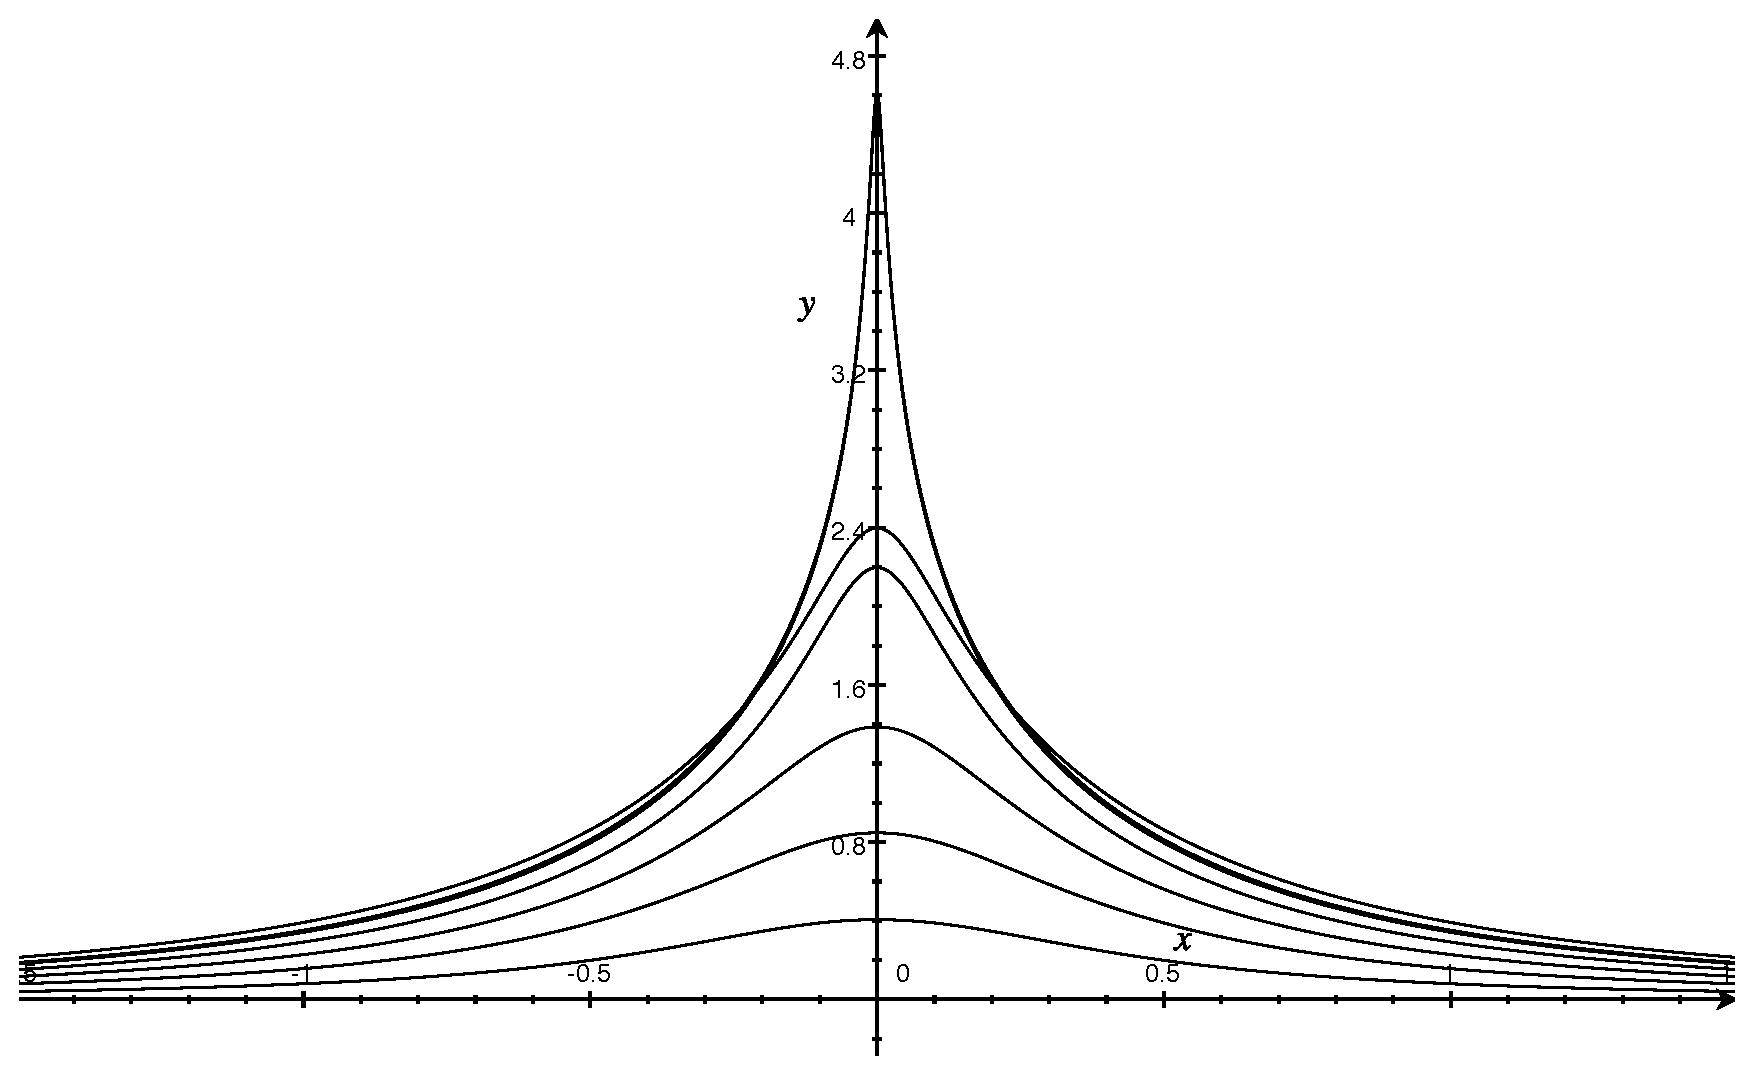
\includegraphics[width=0.48\linewidth]{Figs/Grapher/ModelGreen/reg.eps}
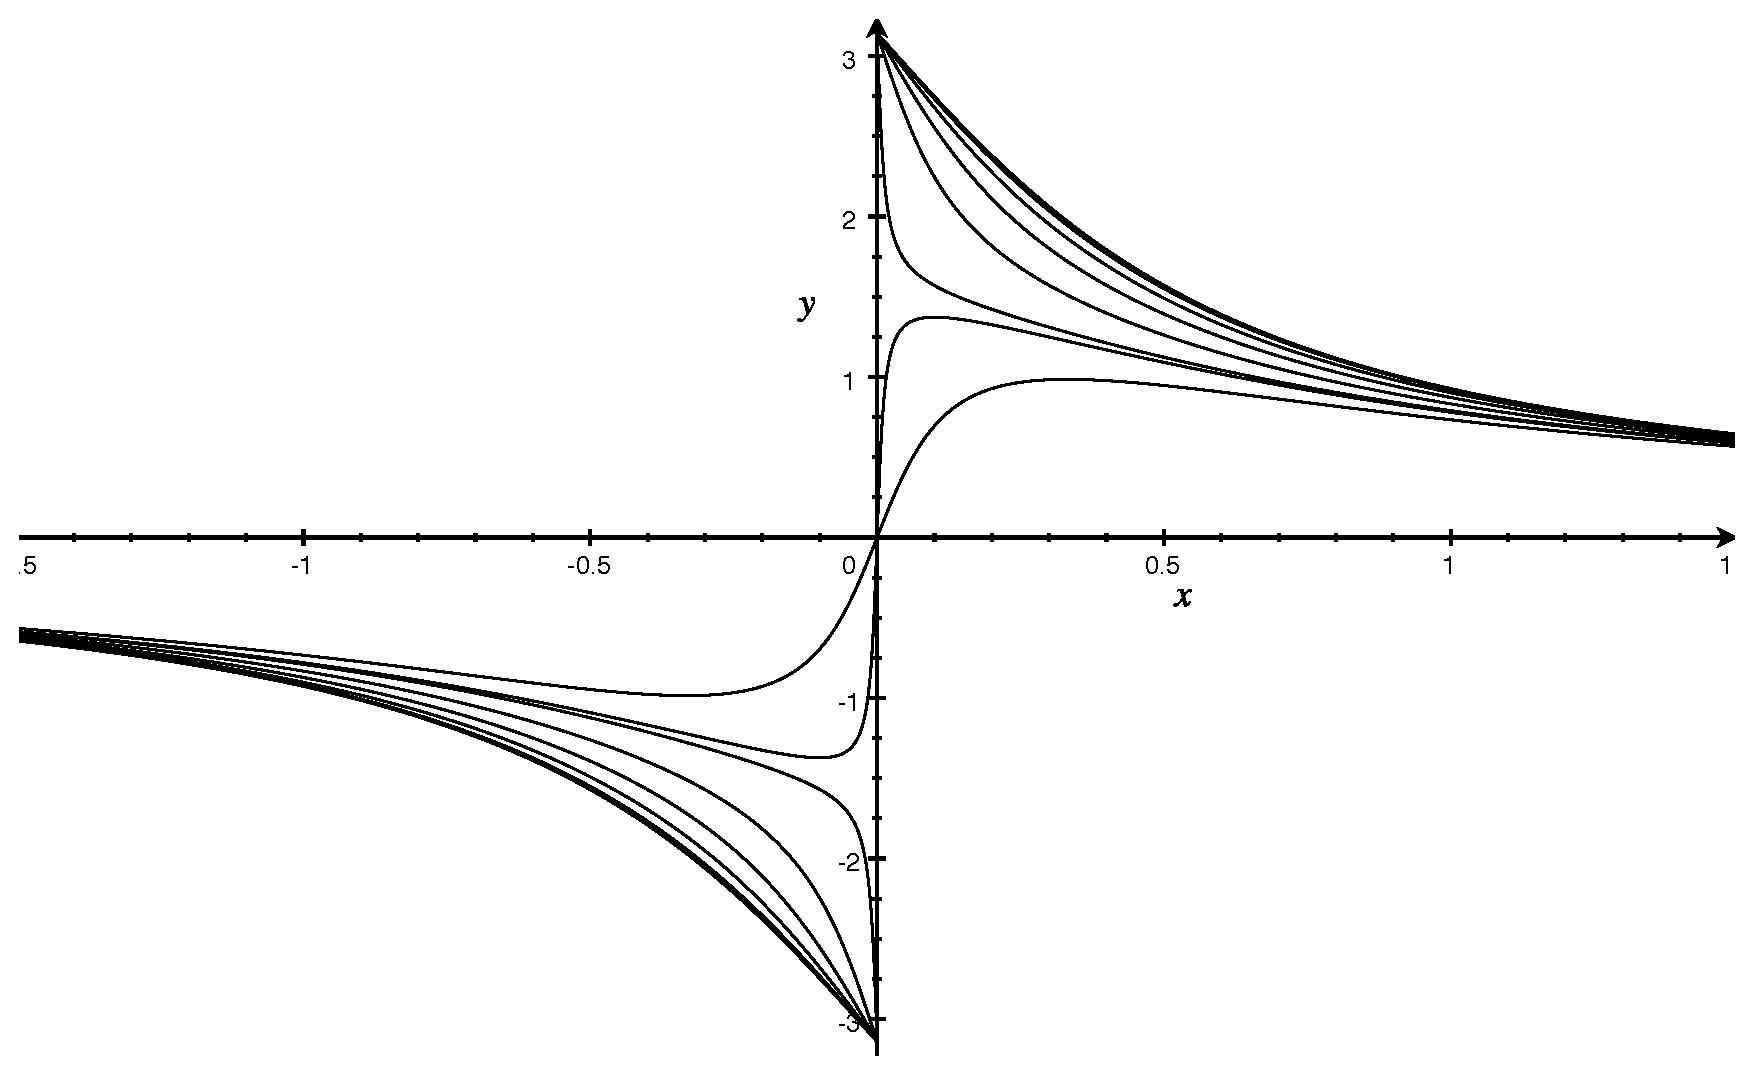
\includegraphics[width=0.48\linewidth]{Figs/Grapher/ModelGreen/img.eps}
\end{center}
\caption{\label{fig:modelgreen}Negative real part (left) and negative imaginary
  part (right) of the Greens function with a constant density of
  states of width $W=1$, centered at
  $E=\{0,0.1,0.2,0.3,0.49,0.51,0.6\}$.}
\end{figure}
The real part is symmetric about
the origin, while the imaginary part is antisymmetric. This is
consistent with $\mat{G}(-i\omega_\nu)=\mat{G}^\dagger(-i\omega_\nu)$.

The imaginary part exhibits a
step at the origin from $\pi/W$ to $\pi/W$ for metallic systems, that is
for a finite density of states at the origin.  For an insulating
system the imaginary part of the Green's function is smooth and has a
finite slope at the origin. 

The real part is positive if the band is
centered above the chemical potential and it is negative if it is
centered below. The real part vanishes if the density of states at the
Fermi level. The real part becomes spiky exactly when the band
touches the Fermi level. As the density of states shifts further to
positive energies, the Greens function grows further in the tails, but
it shrinks in the central region.


\petertt{The following is not correct! Please check!}

Limiting cases
\begin{itemize}
\item $\hbar\omega\rightarrow 0$:

We use the expansion of the arcus tangens
\footnote{
\begin{eqnarray}
  atan(x)&=&y\quad\Rightarrow\quad y=tan(x)=\frac{\sin(x)}{\cos(x)}
\nonumber\\
x&=&\frac{1}{\frac{\pi}{2}-y}+O(y-\frac{\pi}{2})^2
\quad\Rightarrow\quad 
y\approx\frac{\pi}{2}-\frac{1}{x}\quad\text{for $x\rightarrow+\infty$}
\nonumber\\
x&=&\frac{1}{y+\frac{\pi}{2}}+O(y+\frac{\pi}{2})^2
\quad\Rightarrow\quad 
y\approx-\frac{\pi}{2}+\frac{1}{x}\quad\text{for $x\rightarrow-\infty$}
\end{eqnarray}
} and the expansion of the logarithm
\footnote{
\begin{eqnarray}
\ln\left[\frac{a+x}{b+x}\right]\approx
\ln\left[\frac{a}{b}\right]+\left(\frac{1}{a}+\frac{1}{b}\right)x+O(x^2)
\end{eqnarray}
}.
\begin{eqnarray}
G_{a,b}(i\omega_\nu)&=&
\frac{S^{-1}_{a,b}}{W}
\biggl\lbrace
+\frac{1}{2}\ln\left[
\frac{(\hbar\omega)^2+(E-W/2)^2}{(\hbar\omega)^2+(E+W/2)^2}
\right]
-i \left[\atan\left(\frac{E+W/2}{\hbar\omega}\right)
-\atan\left(\frac{E-W/2}{\hbar\omega}\right)\right]
\biggr\rbrace
\nonumber\\
%
&\approx&
\frac{S^{-1}_{a,b}}{W}
\biggl\lbrace
+\frac{1}{2}\ln\left[\left(
\frac{(E-W/2)}{(E+W/2)}\right)^2
\right]
+\frac{1}{2}\left[\frac{1}{(E-W/2)^2}-\frac{1}{(E+W/2)^2}\right]\hbar\omega^2
\nonumber\\
&&-i \left[\frac{\pi}{2}-\frac{\hbar\omega}{E+W/2}
\underbrace{
-\frac{\pi}{2}+\frac{\hbar\omega}{E-W/2}
}_{\text{times -1 for insulators}}\right]
\biggr\rbrace
\nonumber\\
%
&\approx&
\frac{S^{-1}_{a,b}}{W}
\biggl\lbrace
+\ln\left[
\frac{(E-W/2)}{(E+W/2)}
\right]
+\frac{EW}{\left(E^2-\left(\frac{W}{2}\right)^2\right)^2}\hbar\omega^2
-i 
\begin{cases}
\frac{W}{E^2-\left(\frac{W}{2}\right)^2}\hbar\omega
&\text{for insulators}\\
\pm\pi-\frac{4|E|}{E^2-\left(\frac{W}{2}\right)^2}\hbar\omega
&\text{for metals}\\
\end{cases}
\hspace{0.3cm}\biggr\rbrace
\nonumber\\
\end{eqnarray}
%
\item $\hbar\omega\rightarrow \infty$:
\begin{eqnarray}
G_{a,b}(i\omega_\nu)&=&
\frac{S^{-1}_{a,b}}{W}
\biggl\lbrace
+\frac{1}{2}\ln\left[
\frac{(\hbar\omega)^2+(E-W/2)^2}{(\hbar\omega)^2+(E+W/2)^2}
\right]
-i \left[\atan\left(\frac{E+W/2}{\hbar\omega}\right)
-\atan\left(\frac{E-W/2}{\hbar\omega}\right)\right]
\biggr\rbrace
\nonumber\\
%
&\approx&
\frac{S^{-1}_{a,b}}{W}
\biggl\lbrace
-EW(\hbar\omega)^{-2}
-i W (\hbar\omega)^{-1}
\biggr\rbrace
%
\nonumber\\
&\approx&
S^{-1}_{a,b}
\biggl\lbrace
-E(\hbar\omega)^{-2}
-i  (\hbar\omega)^{-1}
\biggr\rbrace
\end{eqnarray}
\end{itemize}

%====================================================================
\newpage
\section{Enforce constraints by minimizing deviation from the density matrix}
%====================================================================

\begin{eqnarray}
F=\sqrt{\sum_{a,b} \Delta\rho_{a,b}\Delta\rho_{b,a}}
\end{eqnarray}

\begin{eqnarray}
dF&=&\frac{1}{2F}\sum_{a,b} 
\biggl[\frac{\partial\Delta\rho_{a,b}}{\partial\Gamma_{\gamma,\delta}}
       \Delta\rho_{b,a}
+\Delta\rho_{a,b}\frac{\partial\Delta\rho_{b,a}}{\partial\Gamma_{\gamma,\delta}}
       \biggr]d\Gamma_{\gamma,\delta}
\nonumber\\
&=&\frac{1}{2F}2\sum_{\gamma,\delta}\sum_{a,b} 
\biggl[\frac{\partial\Delta\rho_{a,b}}{\partial\Gamma_{\gamma,\delta}}
 \Delta\rho_{b,a}
       \biggr]d\Gamma_{\gamma,\delta}
\end{eqnarray}

Now we make use of the definition of $\Delta\mat{\rho}$
\begin{eqnarray}
\Delta\mat{\rho}
&=&k_BT\sum_\nu\e{i\hbar\omega\beta0^+}
\biggl[
\underbrace{\Bigl((i\hbar\omega_\nu+\mu)\mat{S}-\mat{\bar{h}}
+\mat{\Gamma}-\mat{\Sigma}(i\omega_\nu)\Bigr)^{-1}}_{\mat{G}(i\omega_\nu)}
-\underbrace{\Bigl((i\hbar\omega_\nu+\mu)\mat{S}-\mat{\bar{h}}
\Bigr)^{-1}}_{\mat{\bar{{G}}(i\omega_\nu)}}\biggr]
\nonumber\\
d(\Delta\mat{\rho})
&=&
k_BT\sum_\nu\e{i\hbar\omega\beta0^+}
\biggl[-\mat{G}d\mat{\Gamma}\mat{G}\biggr]
=-
k_BT\sum_\nu\mat{G}(i\omega_\nu)d\mat{\Gamma}
\mat{G}(i\omega_\nu)
\end{eqnarray}

\begin{eqnarray}
dF
&=&\frac{1}{F}\sum_{a,b,\gamma,\delta} 
\biggl[-k_BT
\sum_\nu G_{a,\gamma}(i\omega_\nu)d\Gamma_{\gamma,\delta}
G_{\delta,b}(i\omega_\nu)
 \Delta\rho_{b,a}  \biggr]
\nonumber\\
&=&\sum_{\gamma,\delta} \biggl[-\frac{1}{F}\sum_{a,b} 
\biggl[k_BT\sum_\nu
G_{\delta,b}(i\omega_\nu) \Delta\rho_{b,a}
G_{a,\gamma}(i\omega_\nu)\bigr]
       \biggr]d\mat{\Gamma}_{\gamma,\delta}
\end{eqnarray}


The ``optimum'' search direction is the one with the largest (negative)
projection on the gradient.
\begin{eqnarray}
d\mat{\Gamma}^{opt}=+\left[\frac{1}{F}k_BT\sum_\nu
\mat{G}(i\omega_\nu) \Delta\mat{\rho}\;\mat{G}(i\omega_\nu)\right]^\dagger
\end{eqnarray}


%====================================================================
\chapter{Usage}
%====================================================================
%====================================================================
\subsection{Control file}
%====================================================================
A typical control file looks as follows. The DMFT object is activated
by the block \verb|!NTBO| with the value \verb|MODUS='DMFT'|. The DMFT
interface requires a finite temperature calculation, which is
specified by the \verb|!MERMIN| block, where the temperature is
specified.  A finite temperature calculation requires
\verb|SAFEORTHO=T|, so that the wave function dynamics converges to
eigenstates of the Hamiltonian.
\begin{verbatim}
!CONTROL
  !GENERIC NSTEP=500  DT=5. START=F  !END 
  !FOURIER EPWPSI=30. CDUAL=2.0 !END
  !DFT TYPE=10  
     !NTBO MODUS='DMFT' !END   
  !END 
  !PSIDYN STOP=T FRIC=.05 SAFEORTHO=F
    !AUTO FRIC(-)=0.3 FACT(-)=0.97 FRIC(+)=0.3 FACT(+)=1.0 MINFRIC=0.05 !END
  !END
  !MERMIN T[K]=4000. ADIABATIC=T RETARD=10. !END
!end
!EOB
\end{verbatim}

%====================================================================
\subsection{Structure file}
%====================================================================
A typical structure file may look as follows. New are the \verb|!NTBO|
subblocks.
\begin{verbatim}
!STRUCTURE 
  !GENERIC  LUNIT[AA]=   3.8   EUNIT[EV]=T !END
  !OCCUPATIONS EMPTY=10 NSPIN=2 SPIN[HBAR]=1.5 !END
  !KPOINTS DIV=1 1 1 SHIFT=1 1 1 !END
  !SPECIES NAME='CA' ID='CA_HBS_SC' NPRO=2 2 1 
    !NTBO NOFL=1 0 0 RAUG/RCOV=0.8 RTAIL/RCOV=1.4 TAILLAMBDA=2. 1.
          CV=F FOCKSETUP=F  !END 
  !END
  !SPECIES NAME='MN' ID='MN_HBS' NPRO=1 1 1 
     !NTBO NOFL=1 0 1 RAUG/RCOV=1.2 RTAIL/RCOV=1.4 TAILLAMBDA=2. 1.
           LHFWeiGHT=0.25 CV=F FOCKSETUP=F !END 
  !END
  !SPECIES NAME='O_' ID='O_.75_6.0'  NPRO=1 1 0
    !NTBO NOFL=1 1  RAUG/RCOV=1.2 RTAIL/RCOV=1.4 TAILLAMBDA=2. 1.
           CV=F FOCKSETUP=F !END 
  !END
  !LATTICE T=  1.0000        0.0000        0.0000000000
               0.0000        1.0000        0.0000000000
               0.0000        0.0000        1.0000000000 !END
  !ATOM NAME= 'CA1'   R=   0.0  0.0 0.0 !END
  !ATOM NAME= 'MN1'   R=   0.5  0.5 0.5 !END
  !ATOM NAME= 'O_1'   R=   0.0  0.5 0.5 !END
  !ATOM NAME= 'O_2'   R=   0.5  0.0 0.5 !END
  !ATOM NAME= 'O_3'   R=   0.5  0.5 0.0 !END
  !ORBPOT_X
    !POT ATOM='MN(UP)1' VALUE=+.2 TYPE='D' RC=1.5 S=1 !END
  !END
!END 
!EOB
\end{verbatim}



%% %=============================================================
%% \subsubsection{Problems:}
%% %=============================================================
%% \begin{itemize}
%% \item the density matrix obtained from the Matsubara sum has
%%   eigenvalues that lie beyond the interval $[0,1]$. Tests for
%%   Matsubara sums hower shows that the spectrum of occupations should
%%   be smaller for a finite sum that that the true result.
%% %
%% \item for a given self energy the density-matrix constraint may not be
%%   fulfillable. 
%% %
%% \item If we set $\Gamma$ and $Y^{(2)}$ to zero, the optimization of the
%%   self energy is almost decoupled from that of the density matrix.

%% Thus we may consider to replace the equation of motion for the
%% Lagrange multipliers by a discrete transformation.
%% \end{itemize}

%% %=============================================================
%% \newpage
%% \subsection{Linear stability analysis}
%% %=============================================================
%% It is not clear if these dynamical equations approach a fix point if a
%% friction is applied. The reason is (1) that it is not proven that the
%% functional is a minimum with respect to the self energy and (2) the
%% dynamics for the constraint equation is not derived from a minimum
%% principle.

%% The two problematic cases are related to self energy and Lagrange
%% multipliers. Therefore we should analyze the dynamics within this
%% subspace for a fixed one-particle density matrix. In order to
%% understand the dynamics we do a linear stability analyses about a
%% fixed point.

%% We linearize $\bar{\mat{\rho}}$ \eq{eq:defrhobar} about the equilibrium
%% self energy. For the second differential equation, we use
%% \eq{eq:quantityxforderivatives} and expand about $\mat{Y}=0$, with $Y$
%% defined in \eq{eq:defbigy}.
%% \petertt{In the following there is a mixup with $\beta$'s!!}

%% \begin{eqnarray}
%% m_\Gamma\delta\ddot{\Gamma}_{n,n'}
%% &=&\frac{1}{\beta}\sum_\nu\sum_{a,b}
%% \underbrace{
%% \Bigl[
%% \sum_{m,m'} G_{n,m}(i\omega_\nu)\langle\psi_m|\bar{\pi}_a\rangle
%% \langle\bar{\pi}_b|\psi_{m'}\rangle G_{m',n'}(i\omega_\nu)\Bigr]
%% }_{B_{b,a,n',n}(i\omega_\nu)}
%% \delta\Delta\Sigma_{a,b}(i\omega_\nu)
%% \nonumber
%% \\
%% m_\Sigma\delta\Delta\ddot{\Sigma}_{a,b}(i\omega_\nu)
%% &=&\sum_{n,n'}\underbrace{
%% \Bigl[\sum_{m,m'}
%% \langle\bar{\pi}_a|\psi_{m}\rangle G_{m,n}(i\omega_\nu)
%% G_{n',m'}(i\omega_\nu)\langle\psi_{m'}|\bar{\pi}_b\rangle
%% \Bigr]}_{B_{a,b,n,n'}(i\omega_\nu)}\delta\Gamma_{n,n'}
%% \end{eqnarray}

%% After a Fourier ttransform in time we obtain the following matrix equation
%% \begin{eqnarray}
%% \left(\begin{array}{cccc}
%% \beta m_\Gamma\omega^2 & B^{\dagger,\dagger}(i\omega_1) 
%%                 & B^{\dagger,\dagger}(i\omega_2) &\ldots\\
%% B(i\omega_1) & m_\Sigma\omega^2 & 0 & \ldots\\
%% B(i\omega_2) & 0&m_\Sigma\omega^2 &  \ldots\\
%% \vdots &\vdots & 0 & 
%% \end{array}\right)
%% \left(\begin{array}{c}
%% \Gamma \\ \Sigma(i\omega_1)\\ \Sigma(i\omega_2) \\ \vdots
%% \end{array}\right)
%% =0
%% \end{eqnarray}
%% From the lower equation, we obtain
%% \begin{eqnarray}
%% \Sigma(i\omega_\nu)=\frac{1}{m_\Sigma\omega^2}B(i\omega_\nu)\Gamma
%% \end{eqnarray}
%% which we insert into the uppermost equation
%% \begin{eqnarray}
%% &&\Bigl[m_\Gamma\omega^2-\sum_\nu B^{\dagger,\dagger}(i\omega_\nu) 
%% \frac{1}{m_\Sigma\omega^2}B(i\omega_\nu)\Bigr]\Gamma=0
%% \nonumber
%% \\
%% &&\sum_{p,p'}\biggl\lbrace
%% m_\Gamma\omega^2\delta_{n,p}\delta_{n',p'}
%% -\frac{1}{\beta}\sum_{\nu}
%% \sum_{a,b}\Bigl[
%% \sum_{m,m'} G_{n,m}(i\omega_\nu)\langle\psi_m|\bar{\pi}_a\rangle
%% \langle\bar{\pi}_b|\psi_{m'}\rangle G_{m',n'}(i\omega_\nu)\Bigr]
%% \nonumber\\
%% &&\hspace{3cm}\cdot
%% \frac{1}{m_\Sigma\omega^2}
%% \Bigl[\sum_{m,m'}
%% \langle\bar{\pi}_a|\psi_{m}\rangle G_{m,p}(i\omega_\nu)
%% G_{p',m'}(i\omega_\nu)\langle\psi_{m'}|\bar{\pi}_b\rangle
%% \Bigr]
%% \biggr\rbrace\Gamma_{p,p'}=0
%% \nonumber
%% \\
%% \Rightarrow&&\sum_{p,p'}\biggl\lbrace
%% m_\Gamma m_\Sigma \omega^4\delta_{n,p}\delta_{n',p'}
%% -
%% \frac{1}{\beta}\sum_{\nu}
%% \Bigl[
%% \sum_{a,m,q}G_{n,m}(i\omega_\nu)\langle\psi_m|\bar{\pi}_a\rangle
%% \langle\bar{\pi}_a|\psi_{q}\rangle G_{q,p}(i\omega_\nu)\Bigr]
%% \nonumber\\
%% &&\hspace{3cm}\cdot
%% \Bigl[\sum_{b,m',q'}
%% G_{p',q'}(i\omega_\nu)\langle\psi_{q'}|\bar{\pi}_b\rangle
%% \langle\bar{\pi}_b|\psi_{m'}\rangle G_{m',n'}(i\omega_\nu)\Bigr]
%% \biggr\rbrace\Gamma_{p,p'}=0
%% \end{eqnarray}
%% This equation factorizes according to the Bloch vectors.

%% The physical meaning of 
%% \begin{eqnarray}
%% \sum_{b,m',q'}
%% &&G_{p',q'}(i\omega_\nu)\langle\psi_{q'}|\bar{\pi}_b\rangle
%% \langle\bar{\pi}_b|\psi_{m'}\rangle G_{m',n'}(i\omega_\nu)
%% \\
%% &=&\left.\frac{d}{dV}\right|_{V=0}
%% \Bigl[\Bigl(\mat{G}(i\omega_\nu)\Bigr)^{-1}_{n',p'}
%% -\sum_{a,b}\langle\psi_{n'}|\bar{\pi}_a\rangle V\delta_{a,b}
%% \langle\bar{\pi}_b|\psi_{p'}\rangle
%% \Bigr]^{-1}_{p',n'}
%% \end{eqnarray}
%% is that of the response of the Green's function to a constant external
%% potential acting on the orbitals in the correlated subspace.

%% This dynamics is unstable. The forces point in the angular direction
%% and increase with the distance from the center. Thus the centrifugal
%% force shifts the dynamics to increasingly larger orbits.
%% \begin{center}
%% {\tiny
%% \begin{verbatim}
%%        program dyn
%%        implicit none
%%        integer(4),parameter :: niter=10000
%%        real(8)   ,parameter :: dt=1.d0
%%        real(8)   ,parameter :: m=-1.d0
%%        real(8)   ,parameter :: anne=5.d0
%%        real(8)   ,parameter :: c1=1.d0,c2=-1.d0
%%        integer(4)           :: iter
%%        real(8)              :: x0(2),xp(2),xm(2),f(2)
%% !      *************************************************************************
%%        x0=(/1.d0,0.d0/)
%%        xm=x0
%%        do iter=1,niter
%% !        == write ========================
%%          write(*,fmt='(i5,2e20.5)')iter,x0
%% !        == forces ======================
%%          f(1)=-c1*x0(2)
%%          f(2)=-c2*x0(1)
%% !        == propagate
%%          xp=(x0*2.d0-xm*(1.d0-anne)+f*dt**2/m)/(1.d0+anne)
%% !        == switch
%%          xm=x0
%%          x0=xp
%%       enddo
%%       stop
%%       end
%% \end{verbatim}}
%% \end{center}

%% Conceivable is to fix the self energy and allow the density matrix to
%% adjust, including the Lagrange parameters. The Lagrange parameters act
%% as forces for an outer loop in which the self-energy is optimized.




%==============================================================================
\chapter{Bloch representation}
%==============================================================================



%====================================================================
\chapter{Traditional formulation of the dynamical mean-field theory}
%====================================================================
\index{dynamical mean-field theory}
The loop of solver takes as input a local Greens function and a
U-tensor. It produces the value of the Luttinger-Ward functional, and
its derivatives of the Luttinger-Ward functional with respect to
Greens function and U-tensor.

The algorithm is the following
\begin{enumerate}
\item choose a hybridization function $\Delta^{in}(i\omega_\nu)$
\item calculate an output Greens function $\mat{G}^{out}$ as
  follows\footnote{(D. Vollhardt \textit{Dynamical Mean Field Theory
      for Strongly Correlated Materials} in \textit{The LDA+DMFT
      Approach to Strongly Correlated Materials'} E. Pavarini,
    E. Koch, D. Vollhardt and A. Lichtenstein Eds, Forschungszentrum
    Juelich 2011. Eq. 23.ff)}: \petertt{Caution, I
      generalized Dieter's Equations without checking. Signs, factors,
      indices, etc. may be wrong!}
\begin{eqnarray*}
G^{out}_{\alpha,\beta}(i\omega_\nu)&:=&
-\frac{1}{Z}\int\prod_{\gamma} Dc^*_\gamma Dc_\gamma\;
c_\alpha(i\omega_\nu)c^*_\beta(i\omega_\nu) \e{-S_{loc}}
\\
Z&=&\int\prod_{\gamma} Dc^*_\gamma Dc_\gamma\;\e{-S_{loc}}
\\
S_{loc}&=&-\int_0^\beta d\tau_1\int_0^\beta d\tau_2\;
\sum_{\alpha,\beta}c^*_\alpha(\tau_1)
\Bigl[
i\hbar\omega_\nu\delta_{\alpha,\beta}-\Delta^{in}_{\alpha,\beta}(i\omega_\nu)
\Bigr]
c_\beta(\tau_2)
\nonumber\\
&&-\int_0^\beta d\tau \sum_{\alpha,\beta,\gamma,\delta}
U_{\alpha,\beta,\delta,\gamma}
 c^*_\alpha c^*_\beta c_\gamma c_\delta
\end{eqnarray*}
Note, that only the hybridization function $\mat{\Delta}^{in}$ and the
  U-tensor enter in this calculation. The only result is the output
  Greens function $\mat{G}^{out}$.
%
\item Convert the Green's function into a self energy $\mat{\Sigma}^{out}$
  using Dyson's equation
\begin{eqnarray}
\Sigma^{out}_{\alpha,\beta}(i\omega_\nu)
:=-\Bigl(G^{out}(i\omega_\nu)\Bigr)^{-1}_{\alpha,\beta}
+i\hbar\omega_\nu\delta_{\alpha,\beta}
-\Delta^{in}_{\alpha,\beta}(i\omega_\nu)
\label{eq:sigmaout}
\end{eqnarray}
%
\item Use the Greens function $\mat{G}$ passed
  to the solver as input argument (not
  $\mat{G}^{out}$!)  to extract a new
  hybridization function $\mat{\Delta}^{out}$
\begin{eqnarray}
\Delta^{out}_{\alpha,\beta}(i\omega_\nu)
:=-\Bigl(G(i\omega_\nu)\Bigr)^{-1}_{\alpha,\beta}
+i\hbar\omega_\nu\delta_{\alpha,\beta}-\Sigma^{out}_{\alpha,\beta}(i\omega_\nu)
\label{eq:deltaout}
\end{eqnarray}
\end{enumerate}


The steps given above yield a unique mapping from $\Delta^{in}$ to
$\Delta^{out}$. In other words the output hybridization function is a
unique functional of the input hybridization function, the input
Greens function and the U-tensor.
\begin{eqnarray}
\mat{\Delta}^{out}=F[\mat{\Delta}^{in},\mat{G},\mat{U}]
\end{eqnarray}


The mapping depends on exactly two quantities, namely
the input Green's function and the U-tensor. Self-consistency yields the 
fixed point $\Delta^{out}=\Delta^{in}$ of this mapping.
At this fixed point, \eq{eq:deltaout} and \eq{eq:sigmaout} yield
\begin{eqnarray}
G^{out}_{\alpha,\beta}(i\omega_\nu)&=&G_{\alpha,\beta}(i\omega_\nu)
\end{eqnarray}
and 
\begin{eqnarray}
G_{\alpha,\beta}(i\omega_\nu)
=\biggl[
i\hbar\omega_\nu\mat{1}
-\mat{\Sigma}^{out}(i\omega_\nu)
-\mat{\Delta}^{in}(i\omega_\nu)
\biggr]^{-1}_{\alpha,\beta}
\;.
\end{eqnarray}

%==============================================================================
\chapter{Conjugate-gradient method}
%==============================================================================
The conjugate-gradient method is used to determine the
constraints. 


%==============================================================================
\subsection{Wirtinger Calculus}
%==============================================================================
Here, we re-derive it for a real function of a complex vector, because
this is not usually written down explicitely.  We make use of the
\textbf{Wirtinger calculus}\index{Wirtinger calculus} in that we
express the variation of a real function $F$ of a complex argument $z=a+ib$
in the form
\begin{eqnarray}
dF(a,b)&=&\frac{dF}{da}da+\frac{dF}{db}db
\nonumber\\
&=&\frac{1}{2}\Bigl(\frac{dF}{da}-i\frac{dF}{db}\Bigr)\Bigl(da+ib\Bigr)
+\frac{1}{2}\Bigl(\frac{dF}{da}+i\frac{dF}{db}\Bigr)\Bigl(da-ib\Bigr)
\nonumber\\
&=&\frac{dF}{dz}dz+ \frac{dF}{dz^*}dz^*=dF(z,z^*)
\end{eqnarray}
which defines the \textbf{Wirtinger derivatives}\index{Wirtinger derivatives}
\begin{eqnarray}
\frac{dF}{dz}&=&\frac{1}{2}\Bigl(\frac{dF}{da}-i\frac{dF}{db}\Bigr)
\nonumber\\
\frac{dF}{dz^*}&=&\frac{1}{2}\Bigl(\frac{dF}{da}+i\frac{dF}{db}\Bigr)
\end{eqnarray}


We define the force in the Wirtinger calculus as
\begin{eqnarray}
f=-\frac{dF}{dz}
\end{eqnarray}
so that
\begin{eqnarray}
dF=-f^*dz-dz^*f
\end{eqnarray}


%==============================================================================
\subsection{Definition of the problem}
%==============================================================================
The goal is to determine the minimum of a real quadratic function
$F(\vec{x})$ of a complex vector $\vec{x}$
\begin{eqnarray}
F(\vec{x})=\vec{x}^*\mat{A}\vec{x}-\vec{b}^*\vec{x}-\vec{x}^*\vec{b}
\end{eqnarray}
where $\mat{A}$ is a positive definite, hermitean matrix.

The condition for a minimum is
\begin{eqnarray}
dF(\vec{x},\vec{x}^*)
=d\vec{x}^*\Bigl(\mat{A}\vec{x}-\vec{b}\Bigr)
+\Bigl(\vec{x}^*\mat{A}-\vec{b}^*\Bigr)d\vec{x}\stackrel{!}{=}0
\nonumber\\
\Rightarrow\quad
\mat{A}\vec{x}-\vec{b}=0\qquad\text{and}\qquad \vec{x}^*\mat{A}-\vec{b}^*=0
\end{eqnarray}
Because the function $F$ is real, the two equations obtained from the
variation of $\vec{x}$ and $\vec{x}^*$ are not indepependent, but both
equations are complex conjugate of each other.


%==============================================================================
\subsection{Minimization on a hyperplane}
%==============================================================================
Given is a $k$-dimensional hyperplane
$\mathcal{D}_k=span\{\vec{d}_1,\ldots,\vec{d}_k\}$, which is spanned
by a set of search directions $\vec{d}_i$. The search directions shall
furthermore be conjugate to each other, i.e.
\begin{eqnarray}
\vec{d}_i^*\mat{A}\vec{d}_j=0\qquad\text{for $i\neq j$}
\label{eq:cgconjugacy}
\end{eqnarray}

All points on the hyperplane can be expressed by
\begin{eqnarray}
\vec{x}(\alpha_1,\ldots,\vec{\alpha}_k)=\sum_{i=1}^k\vec{d}_i\alpha_i
\label{eq:cgxofpalpha}
\end{eqnarray}

The function $F$ can be mapped onto the hyperplane, yielding $F_k$
\begin{eqnarray}
F_k(\vec{\alpha},\vec{\alpha}^*)
=\sum_{i,j} \alpha_i^* \vec{d}^*_i\mat{A}\vec{d}_j\alpha_j
-\sum_j \vec{b}^*\vec{d}_i\alpha_j
-\sum_i \alpha_i^*\vec{d}^*_i\vec{b}
\end{eqnarray}

The minimum condition of $F_k$ on the hyperplane is
\begin{eqnarray}
dF_k
&=&\sum_id\alpha_i^*\biggl(\sum_{j}\vec{d}^*_i\mat{A}\vec{d}_j\alpha_j
-\vec{d}^*_i\vec{b}\biggr)
+\sum_{j} 
\biggl(\sum_{i} \alpha_i^* \vec{d}^*_i\mat{A}\vec{d}_j
-\vec{b}^*\vec{d}_j\biggr)d\alpha_j
\nonumber\\
&\eqrel{eq:cgconjugacy}{=}&
\sum_id\alpha_i^*\biggl(\vec{d}^*_i\mat{A}\vec{d}_i\alpha_i
-\vec{d}^*_i\vec{b}\biggr)
+\sum_{i} 
\biggl( \alpha_i^* \vec{d}^*_i\mat{A}\vec{d}_i
-\vec{b}^*\vec{d}_i\biggr)d\alpha_i
\nonumber\\
dF_k\stackrel{!}{=}0&\Rightarrow&
\alpha_i=\frac{\vec{d}^*_i\vec{b}}{\vec{d}^*_i\mat{A}\vec{d}_i}
\label{eq:cgalhaofab}
\end{eqnarray}

Thus, we obtain the minimum in the hyperplane as 
\begin{eqnarray}
\vec{x}_k&
\stackrel{Eq.~\ref{eq:cgxofpalpha},\ref{eq:cgalhaofab}}{=}
&\sum_{i=1}^k\vec{d}_i
\frac{\vec{d}^*_i\vec{b}}{\vec{d}^*_i\mat{A}\vec{d}_i}
\end{eqnarray}

We can also determine the minima in hyperplanes with successivly  
higher dimensions in the form
\begin{eqnarray}
\vec{x}_k&=&
\vec{x}_{k-1}+\vec{d}_k\alpha_k
=\vec{x}_{k-1}+\vec{d}_k
\frac{\vec{d}^*_k\vec{b}}{\vec{d}^*_k\mat{A}\vec{d}_k}
\end{eqnarray}

In practice we do not wish to use $\vec{b}$ and $\mat{A}$, but only
the values of $F$ and its derivatives at specific points. For this
purpose, I exploit that the force
$\vec{f}=-\vec{\nabla}_{\vec{x}^*}F$, also called the
\textbf{residuum}\index{residuum}, is orthogonal to the previous
search direction.
\begin{eqnarray}
\vec{f}_k=-\left.\vec{\nabla}_{\vec{x}^*}\right|_{\vec{x}_k,\vec{x}_k^*} F
=\vec{b}-\mat{A}\vec{x}_k
\label{eq:cgforceofab}
\end{eqnarray}

Because
\begin{eqnarray}
dF_k=
-\sum_i d\alpha_i^* \vec{d}_i^* \vec{f}_k
-\sum_i \vec{f}_k^* \vec{d}_id\alpha_i
\end{eqnarray}
any component of $\vec{f}_k$ on $\vec{d}_i^*$, i.e. any finite value
of $\vec{d}^*_i\vec{f}_k$, would allow one to lower the value of $F_k$
by changing $\alpha_k$. This, however, would contradict the assumption
that $\vec{x}_k$ is the minimum of $\vec{F}_k$.

Therefore, we conclude that the force is orthogonal to all ``previous''
search directions
\begin{eqnarray}
\vec{d}_i^*\vec{f}_k=\vec{f}_k^*\vec{d}_i=0\quad\text{for $i\le k$}
\label{eq:cgorthogonalityforceandsearch}
\end{eqnarray}

In particular, we can determine $\vec{x}_k$ and $\alpha_k$ from 
\begin{eqnarray}
\vec{x}_k&=&\vec{x}_{k-1}+\vec{d}_k\alpha_k
\label{eq:cgxkwithalphaka}
\\
\vec{f}_k^*\vec{d}_k&=&0\leadsto\alpha_k
\label{eq:cgxkwithalphakb}
\end{eqnarray}

%==============================================================================
\subsection{Determine next search direction}
%==============================================================================
The next search direction shall include the last force.  Furthermore,
it must obey the conjugacy condition to all previous search
directions. This can be accomplished by mixing in the previous search
directions
\begin{eqnarray}
\vec{d}_{k+1}=\vec{f}_k+\sum_{j=1}^{k}\vec{d}_j\beta_j
\label{eq:cgnewsearch0}
\end{eqnarray}
where the coefficients $\beta_j$ are determined so that
\begin{eqnarray}
\vec{d}^*_i\mat{A}\vec{d}_{k+1}=0\quad\text{for $i\le k$}
\end{eqnarray}

\begin{eqnarray}
\vec{d}^*_i\mat{A}\vec{d}_{k+1}&\eqrel{eq:cgnewsearch0}{=}&
\vec{d}^*_i\mat{A}\vec{f}_k
+\sum_{j=1}^{k}\vec{d}^*_i\mat{A}\vec{d}_j\beta_j 
\eqrel{eq:cgconjugacy}{=}
\vec{d}^*_i\mat{A}\vec{f}_k
+\vec{d}^*_i\mat{A}\vec{d}_i\beta_i\stackrel{!}{=}0
\nonumber\\
\Rightarrow\qquad
\beta_i&=&-\frac{\vec{d}^*_i\mat{A}\vec{f}_k}{\vec{d}^*_i\mat{A}\vec{d}_i}
\label{eq:cgbetaofab}
\end{eqnarray}

\begin{eqnarray}
\vec{d}_{k+1}
\stackrel{Eq.~\ref{eq:cgnewsearch0},\ref{eq:cgbetaofab}}{=}
\vec{f}_k-\sum_{j=1}^{k}\vec{d}_j
\frac{\vec{d}^*_j\mat{A}\vec{f}_k}{\vec{d}^*_j\mat{A}\vec{d}_j}
\label{eq:cgnewsearch1}
\end{eqnarray}

It is our goal to express the new search direction without direct
reference to the matrix $\mat{A}$. Therefore, we represent
$\vec{d}^*_j\mat{A}$ by two subsequent forces.
\begin{eqnarray}
\vec{f}_j-\vec{f}_{j-1}&\eqrel{eq:cgforceofab}{=}&
\vec{b}-\mat{A}\vec{x}_j-\vec{b}+\mat{A}\vec{x}_{j-1}
=-\mat{A}(\vec{x}_j-\vec{x}_{j-1})
\eqrel{eq:cgxkwithalphaka}{=}
-\mat{A}\vec{d}_j\alpha_j
\end{eqnarray}


\begin{eqnarray}
\vec{d}_{k+1}\eqrel{eq:cgnewsearch1}{=}\vec{f}_k
-\sum_{j=1}^{k}\vec{d}_j
\frac{\Bigl(\vec{f}_j^*-\vec{f}_{j-1}^*\Bigr)\vec{f}_k}
{\Bigl(\vec{f}_j^*-\vec{f}_{j-1}^*\Bigr)\vec{d}_j}
\label{eq:cgnewsearch2}
\end{eqnarray}

Next, I show that the forces $\vec{f}_k$ are orthogonal to each other,
i.e. $\vec{f}_i^*\vec{f}_j=0$, which will simplify
\eq{eq:cgnewsearch2} by limiting the sum to the last term.

Because the search directions are built up, via
\eq{eq:cgnewsearch0}, from the forces, the forces and search
directions span the same hyperplane.
\begin{eqnarray}
\text{span}\{\vec{d}_1,\ldots,\vec{d}_k\}=
\text{span}\{\vec{f}_0,\ldots,\vec{f}_{k-1}\}
\end{eqnarray}
Because $\vec{f}_k$ is orthogonal to the search directions
$\vec{d}_1,\ldots,\vec{d}_k$, it is also orthogonal to the forces
$\vec{f}_0,\ldots,\vec{f}_{k-1}$. Hence, the forces are orthogonal to
each other.
\begin{eqnarray}
\vec{f}_i^*\vec{f}_j=0\quad\text{for $i\neq j$}
\label{eq:cgorthogonalityforces}
\end{eqnarray}

With the orthogonality conditions \eq{eq:cgorthogonalityforces}, we
can limit the expression for the new search direction to the last term
\begin{eqnarray}
\vec{d}_{k+1}\eqrel{eq:cgnewsearch2}{=}\vec{f}_k
-\vec{d}_k
\frac{\Bigl(\vec{f}_k^*-\vec{f}_{k-1}^*\Bigr)\vec{f}_k}
{\Bigl(\vec{f}_k^*-\vec{f}_{k-1}^*\Bigr)\vec{d}_k}
\label{eq:cgnewsearchHS}
\end{eqnarray}
This is the final expression of
\textbf{Heestenes and Stiefel}\index{Heestenes-Stiefel}.

Using the orthogonality conditions we can also determine variants of
the above equation.  We can go a step further and use
\begin{eqnarray}
\vec{d}_k\eqrel{eq:cgnewsearchHS}{=}\vec{f}_{k-1}+\vec{d}_{k-1}\beta
\label{eq:cgnewsearch3a}
\end{eqnarray}
to transform
\begin{eqnarray}
\Bigl(\vec{f}_k^*-\vec{f}_{k-1}^*\Bigr)\vec{d}_k
\stackrel{\vec{f}_k^*\vec{d}_k=0}{=}
-\vec{f}_{k-1}^*\vec{d}_k
\eqrel{eq:cgnewsearch3a}{=}
-\vec{f}_{k-1}^*\Bigl(\vec{f}_{k-1}+\vec{d}_{k-1}\beta\Bigr)
\stackrel{\vec{f}_{k-1}^*\vec{d}_{k-1}=0}{=}
-\vec{f}_{k-1}^*\vec{f}_{k-1}
\label{eq:cgfromfdtoff}
\end{eqnarray}

With this expression we arrive at the formula of \textbf{Polak and Ribiere}
\index{Polak-Ribiere}.
\begin{eqnarray}
\vec{d}_{k+1}
\stackrel{Eqs.~\ref{eq:cgnewsearchHS},\ref{eq:cgfromfdtoff}}{=}
\vec{f}_k
+\vec{d}_k
\frac{\Bigl(\vec{f}_k^*-\vec{f}_{k-1}^*\Bigr)\vec{f}_k}
{\vec{f}_{k-1}^*\vec{f}_{k-1}}
\label{eq:cgnewsearchPR}
\end{eqnarray}
The sequence of Polak and Ribiere shall be restarted, when the 
$\Bigl(\vec{f}_k^*-\vec{f}_{k-1}^*\Bigr)\vec{f}_k<0$

Using the orthogonality of the forces again, we arrive at the expression of
\textbf{Fletcher and Reeves}\index{Fletcher-Reeves}.
\begin{eqnarray}
\vec{d}_{k+1}\eqrel{eq:cgnewsearchPR}{=}\vec{f}_k
+\vec{d}_k
\frac{\vec{f}_k^*\vec{f}_k}
{\vec{f}_{k-1}^*\vec{f}_{k-1}}
\label{eq:cgnewsearchFR}
\end{eqnarray}

All three expressions are equivalent, if the problem is purely
parabolic. If the problem is nonlinear they provide different
convergence.

\textbf{Most importantly, the sequence must be restarted, whenever the
  denominator vanishes! The sequence can be restarted by removing the
  admixture of the previous search direction, i.e. by setting
  $\beta=0$.}


%==============================================================================
\subsection{Nonlinear Conjugate Gradient Method}
%==============================================================================
The nonlinear conjugate gradient method is the same method, just
applied to a general real function $F(\vec{x})$ instead of a quadratic
function.
For a general function, the orthogonality of the forces is no more
strictly valid. 

The equation of Heestenes-Stiefel and the one of Pollak Ribiere are
strictly identical, because they only require the orthogonality
$\vec{f}_j^*\vec{d}_j$ between search directions and forces in the
same iteration. This is imposed also in the general case.

The equation of Fletcher and Reeves differs from the ones of
Heestenes-Stiefel and Polak-Ribiere, because they assume also that
$\vec{f}_{k-1}\vec{f}_k$, which is not obeyed in the nonlinear case.




%==============================================================================
\subsection{Recipe}
%==============================================================================
\begin{myshadowminipage}{Conjugate gradient scheme}
\begin{enumerate}
\item Start-up: The conjugate gradient iteration is started from an
  arbitrary point, $\vec{x}_0$. At this point the force $\vec{f}_0$ is
  evaluated. The force also defines the first search direction
\begin{eqnarray}
\vec{d}_1=\vec{f}_0
\end{eqnarray}
%
\item Line search for next point $\vec{x}_k$.
\begin{eqnarray}
\vec{x}_k&=&\vec{x}_{k-1}+\vec{d}_k\alpha_k
\label{eq:cgfinalxkwithalphaka}
\\
\vec{f}_k^*\vec{d}_k&=&0\leadsto\alpha_k
\label{eq:cgfinalxkwithalphakb}
\end{eqnarray}
%
\item determine new search direction $\vec{d}_{k+1}$
\begin{eqnarray}
\vec{d}_{k+1}\eqrel{eq:cgnewsearch1}{=}\vec{f}_k+\vec{d}_k\beta_k
\end{eqnarray}
with one of the expressions
\begin{itemize}
\item Fletcher-Reeves
\begin{eqnarray}
\beta_k\eqrel{eq:cgnewsearchFR}{=}
+\frac{\vec{f}_k^*\vec{f}_k}
{\vec{f}_{k-1}^*\vec{f}_{k-1}}
\label{eq:cgfinalnewsearchFR}
\end{eqnarray}
\item Polak-Ribiere
\begin{eqnarray}
\beta_k\eqrel{eq:cgnewsearchPR}{=}
\max\left(0,
+\frac{\Bigl(\vec{f}_k^*-\vec{f}_{k-1}^*\Bigr)\vec{f}_k}
{\vec{f}_{k-1}^*\vec{f}_{k-1}}\right)
\label{eq:cgfinalnewsearchPR}
\end{eqnarray}
The condition that $\beta>0$ has been mentioned by
Shewchuk\cite{shewchuk94_url}.


\item Heestenes-Stiefel
\begin{eqnarray}
\beta_k\eqrel{eq:cgnewsearchHS}{=}
-\frac{\Bigl(\vec{f}_k^*-\vec{f}_{k-1}^*\Bigr)\vec{f}_k}
{\Bigl(\vec{f}_k^*-\vec{f}_{k-1}^*\Bigr)\vec{d}_k}
\label{eq:cgfinalnewsearchHS}
\end{eqnarray}
\end{itemize}
Restart the CG iteration (set $\beta_k=0$) if the denominator
vanishes, or if $\beta_k>0$.
\end{enumerate}
\end{myshadowminipage}


\printindex
\clearpage
\bibliographystyle{unsrtnat} 
 \bibliography{../all}
\end{document}  
 
